\documentclass[12pt,a4paper]{report}
\usepackage[utf8]{inputenc}
\usepackage[T1]{fontenc}
\usepackage{amsmath,amssymb,amsthm}
\usepackage{physics}
\usepackage{bm}
\usepackage{slashed}
\usepackage{hyperref}
\hypersetup{
  colorlinks=true,
  linkcolor=blue,
  citecolor=blue,
  urlcolor=blue
}
\usepackage{geometry}
\usepackage{setspace}
\usepackage{booktabs}
\usepackage{caption}
\usepackage{graphicx}
\usepackage{grffile}
\usepackage{array}

\geometry{margin=2.5cm}
\onehalfspacing

% Figures are not duplicated into this folder; they are picked up directly
% from main_figures/, a regenerated copy dedicated to this expanded
% project so that refreshing figures here can never affect the original
% project/ directory's compiled output.
% Full-page figures ([p]) sit vertically centred on their own page: equal
% stretchable glue above and below the float. These are the standard-class
% values, set explicitly so the layout does not depend on class defaults.
\makeatletter
\setlength{\@fptop}{0pt plus 1fil}
\setlength{\@fpsep}{8pt plus 2fil}
\setlength{\@fpbot}{0pt plus 1fil}
\makeatother

\graphicspath{%
  {../main_figures/constraint_atlas/}%
  {../main_figures/gap_analysis/}%
  {../main_figures/matter_antimatter/}%
}

% Hanging-indent reference entries, per the University of Ibadan citation
% format: first line fully justified, run-over lines indented one tab.
\newcommand{\refitem}[1]{\par\noindent\hangindent=1.27cm\hangafter=1 #1\par\vspace{6pt}}

\title{Unified Constraint Framework for Exotic Spin-Dependent Interactions:\\
Matter--Antimatter Sector Comparison}
\author{Oyewo Temidayo Solomon}
\date{2026}

\begin{document}

% ------------------------------------------------------------------
% TITLE PAGE
% ------------------------------------------------------------------
\begin{titlepage}
\centering
\vspace*{2cm}

{\LARGE \bfseries Unified Constraint Framework for Exotic\\[0.3em]
Spin-Dependent Interactions:\\[0.3em]
Matter--Antimatter Sector Comparison\par}

\vspace{2.5cm}

{\large By\par}

\vspace{0.4cm}

{\Large Oyewo Temidayo Solomon\par}
{\large Matriculation Number: 254010\par}

\vspace{1.5cm}

{\large A thesis submitted to the Department of Physics,\\
Faculty of Science, University of Ibadan,\\
in partial fulfilment of the requirements\\
for the award of the degree of Master of Science in Theoretical Physics\\
of the University of Ibadan\par}

\vspace{2cm}

{\large Supervisor: Professor O.~E. Oyewande\\
Department of Physics\\
University of Ibadan, Nigeria\par}

\vfill

{\large University of Ibadan, Nigeria\\
2026\par}

\end{titlepage}

% ------------------------------------------------------------------
% FRONT MATTER: roman-numeral page numbering (i, ii, iii, ...)
% ------------------------------------------------------------------
\pagenumbering{roman}

% ------------------------------------------------------------------
% DEDICATION
% ------------------------------------------------------------------
\chapter*{Dedication}
\addcontentsline{toc}{chapter}{Dedication}

To everyone who insists that a symmetry as fundamental as CPT deserves to be
checked, not assumed.


% ------------------------------------------------------------------
% ABSTRACT
% ------------------------------------------------------------------
\chapter*{Abstract}
\addcontentsline{toc}{chapter}{Abstract}

Exotic spin-dependent interactions mediated by light, weakly coupled bosons
(axions, axion-like particles, dark photons) are a well-motivated
low-energy signature of physics beyond the Standard Model. Two languages
are used to describe them: the Standard Model Extension (SME), a
relativistic effective field theory of Lorentz and CPT violation, and the
Dobrescu--Mocioiu (DM) classification, a complete basis of sixteen
non-relativistic potentials ($V_1$--$V_{16}$) in which experiments actually
report their bounds. No complete, systematic dictionary previously
connected the two, and no framework existed for using such a dictionary to
compare matter-sector and antimatter-sector constraints as a quantitative
test of CPT symmetry. This thesis develops both.

The Foldy--Wouthuysen transformation is applied to the SME fermion-sector
coefficients $b_\mu$, $d_{\mu\nu}$, $g_{\lambda\mu\nu}$ and $H_{\mu\nu}$ to
derive the non-relativistic Hamiltonian each generates and match it onto the
corresponding DM potential(s). These four are shown to be the complete set
that generates spin-dependent non-relativistic potentials: $a_\mu$,
$c_{\mu\nu}$ and $e_\mu$ appear only in spin-independent terms and $f_\mu$
not at all through third order in $1/m$, so none has an image in the DM
basis. All four
derivations are obtained in full and agree with established results,
including the momentum-dependent $d_{ij}$ and $d_{00}$ components, whose
apparent sign discrepancy against the literature is shown to arise from a
momentum-index convention in the reference result rather than from the
derivation. A dimensionless CPT asymmetry parameter, $A_\alpha =
(g_\alpha^{f}-g_\alpha^{\bar f})/(g_\alpha^{f}+g_\alpha^{\bar f})$, is
defined and, using a purpose-built pipeline (SPINDEP), evaluated against a
compiled database of 283 experimental constraint datasets, 247 of which
enter the analysis, spanning
nitrogen-vacancy-centre magnetometry, torsion balances, atomic
co-magnetometers, positronium spectroscopy, and antimatter experiments,
standardised to a common interaction-range axis.

Only 22 of the 247 analysed datasets involve an antimatter sector, from
which fifteen matter--antimatter pairs could be statistically compared. Every pair shows
a significant asymmetry after correcting for autocorrelation among
interpolated points, yet an analytic argument, confirmed empirically across
all fifteen pairs, shows that $A_\alpha$ built from one-sided experimental
upper bounds cannot by itself distinguish genuine CPT violation from an
ordinary sensitivity gap between the matter- and antimatter-sector
experiments being compared. A gap analysis by fermion sector and by DM
potential identifies the $e$--$N$, $n$--$N$, $p$--$N$, $e$--$n$, $n$--$p$,
and $n$--$n$ sectors,
and the $V_{1a}$, $V_{9+10}$, and $V_{12+13}$ potentials, as the largest
opportunities for new antimatter-sector measurements. The thesis concludes
that the antimatter-sector coverage gap, not statistical power, is the
binding constraint on testing CPT symmetry through exotic spin-dependent
interactions, and offers the mapping table, the database, and the analysis
pipeline as an extensible resource for closing it.

\textbf{Keywords:} Standard Model Extension, Dobrescu--Mocioiu potentials,
Foldy--Wouthuysen transformation, CPT symmetry, exotic spin-dependent
interactions, matter--antimatter asymmetry.


% ------------------------------------------------------------------
% LIST OF FIGURES / LIST OF TABLES
% ------------------------------------------------------------------
\listoffigures
\listoftables

% ------------------------------------------------------------------
% ACKNOWLEDGEMENTS
% ------------------------------------------------------------------
\chapter*{Acknowledgements}
\addcontentsline{toc}{chapter}{Acknowledgements}

I am grateful to my supervisor, Professor O.~E. Oyewande, for guidance
throughout the development of this thesis, and to the Department of
Physics, University of Ibadan, for the academic environment in which this
research was carried out.

I thank the maintainers of the Standard Model Extension data tables and the
authors of the experimental works compiled in the constraint database of
this thesis, without whose careful reporting of bounds this analysis would
not have been possible.

Finally, I thank my family and colleagues for their support and patience
throughout the duration of this programme.


% ------------------------------------------------------------------
% TABLE OF CONTENTS
% ------------------------------------------------------------------
\tableofcontents

% ------------------------------------------------------------------
% CERTIFICATION
% ------------------------------------------------------------------
\chapter*{Certification}
\addcontentsline{toc}{chapter}{Certification}

I certify that this work was carried out by Oyewo Temidayo Solomon in the
Department of Physics, University of Ibadan, Nigeria.

\vspace{3cm}

\noindent\rule{7cm}{0.4pt}\\
\textbf{Professor O.~E. Oyewande}\\
Supervisor\\
Department of Physics\\
University of Ibadan, Nigeria\\
Date: \rule{4cm}{0.4pt}

\vspace{2.5cm}

\noindent\rule{7cm}{0.4pt}\\
\textbf{Head of Department}\\
Department of Physics\\
University of Ibadan, Nigeria\\
Date: \rule{4cm}{0.4pt}


% ------------------------------------------------------------------
% MAIN MATTER: normal (arabic) page numbering restarts at 1 here
% ------------------------------------------------------------------
\clearpage
\pagenumbering{arabic}
\setcounter{page}{1}

% ------------------------------------------------------------------
% CHAPTERS
% ------------------------------------------------------------------
\chapter{Introduction}
\label{ch:introduction}

\section{Background to the Research}

The Standard Model has been tested to extraordinary precision, yet it is
not considered a complete theory because it says nothing about gravity at the quantum level,
it has no dark matter candidate despite dark matter making up roughly a
quarter of the universe's energy budget (Planck Collaboration, 2020), and
it cannot explain why the universe is full of matter and almost no
antimatter. These gaps motivate the search for physics beyond the Standard
Model (BSM), one well-motivated form of which is a class of light, weakly
coupled bosonic fields, such as axions, axion-like particles, and dark
photons, that mediate feeble, long-range \emph{fifth forces}.

This thesis is concerned with a specific subset of fifth forces: those that
couple to fermion spin rather than to charge or mass alone. Spin has no
classical analogue, which makes \emph{exotic spin-dependent interactions}
an unusually clean channel for probing symmetry violation. Two languages
are used to describe such interactions. The Standard Model Extension (SME)
of Colladay and Kostelecký (1997, 1998) is a relativistic effective field
theory that systematically parametrises Lorentz and CPT violation through
fixed background coefficients such as $b_\mu$, $H_{\mu\nu}$, and
$d_{\mu\nu}$. The Dobrescu--Mocioiu (DM) classification (Dobrescu and
Mocioiu, 2006) is a complete, non-relativistic basis of sixteen potentials,
$V_1$--$V_{16}$, in which nearly all laboratory searches for exotic forces
report their bounds. Connecting the two requires the Foldy--Wouthuysen (FW)
transformation (Foldy and Wouthuysen, 1950), the standard technique for
extracting the non-relativistic limit of a relativistic Dirac Hamiltonian.

Separately, antimatter physics has become one of the sharpest available
tools for testing fundamental symmetries. Experiments at CERN, such as BASE
and ALPHA, compare matter and antimatter magnetic moments and spectral
lines at a precision that directly tests charge-parity-time (CPT)
invariance (Smorra \textit{et al.}, 2017; Ahmadi \textit{et al.}, 2017).
Combining these two threads, exotic spin-dependent interaction searches and
antimatter precision physics, opens a regime in which a CPT-violating
interaction would appear as a measurable asymmetry between the coupling
constants measured for matter and for antimatter.

\section{Research Problem and Hypotheses}

Despite over a hundred experiments compiled through 2024 (Cong \textit{et
al.}, 2025), no unified framework systematically translates between the
SME and DM formalisms, and no framework exists for comparing matter-sector
and antimatter-sector constraints on exotic spin-dependent interactions
within a single, quantitative measure of CPT consistency. The SME describes
Lorentz- and CPT-violating physics through operator coefficients that are
not directly expressed as measurable potentials; the DM basis is
experimentally convenient but does not make its relativistic origin
explicit. Prior attempts at a mapping between the two are partial,
restricted to subsets of coefficients or potentials, and no compiled
constraint database exists in a form that allows a direct, standardised
comparison of matter- and antimatter-sector bounds across particle species,
interaction types, and experimental platforms.

This research problem yields two working hypotheses examined in this
thesis. First, that a complete Foldy--Wouthuysen reduction of the four SME
coefficients that generate spin-dependent terms, the CPT-odd $b_\mu$ and
$g_{\lambda\mu\nu}$ and the CPT-even $H_{\mu\nu}$ and $d_{\mu\nu}$, can be
matched, coefficient by coefficient, onto the DM potential basis, and that
the resulting potentials will change sign between matter and antimatter for
the CPT-odd coefficients but not for the CPT-even ones. Second, that a
dimensionless asymmetry parameter $A_\alpha$, computed from currently
published experimental bounds, can be used to test this prediction
quantitatively once matter- and antimatter-sector datasets are compiled
and standardised.

The first hypothesis is confirmed for all four coefficients, with one
clarification about what is being compared. The sign flip for the CPT-odd
$b_\mu$ and $g_{\lambda\mu\nu}$, and its absence for the CPT-even
$H_{\mu\nu}$ and $d_{\mu\nu}$, hold between CPT-conjugate states, in which
the antiparticle's spin is reversed. At the same physical spin the pattern
is reversed, as Kostelecký and Lane (1999b) state
(Section~\ref{sec:results-fw-bmu}). The second
hypothesis is limited by the nature of the data. Published bounds are
one-sided upper limits rather than signed measurements, so $A_\alpha$ alone
cannot always separate a genuine CPT-violating signal from an ordinary gap
in experimental sensitivity (Chapters~3 and~4). This thesis treats that
limitation as a central finding rather than an incidental caveat.

\section{Justification for the Research}

A unified SME--DM mapping gives experimentalists a direct way to translate
a measured or constrained potential into a bound on a relativistic,
symmetry-classified coefficient, and vice versa, rather than relying on
partial, coefficient-specific translations scattered across the
literature. A standardised, cross-platform constraint database removes the
unit and convention inconsistencies that currently make it difficult to
compare bounds from nitrogen-vacancy-centre magnetometry, torsion balances,
atomic co-magnetometers, positronium spectroscopy, and antimatter
spectroscopy on equal footing. Together, these tools enable the first
systematic matter--antimatter comparison of spin-dependent forces and
provide a reusable, extensible pipeline (SPINDEP) rather than a one-off
calculation, one that automatically incorporates future antimatter-sector
measurements as they are published. The results are relevant to ongoing
experimental programmes at CERN (BASE, ALPHA), to precision quantum sensing
laboratories, and to the SME data tables maintained by Kostelecký and
Russell (2011), which this work is intended to complement.

\section{Aims and Objectives}

The primary objective of this research is to develop a unified theoretical
and computational framework that connects Standard Model Extension
coefficients to Dobrescu--Mocioiu spin-dependent potentials and enables
systematic comparison of matter- and antimatter-sector constraints to test
CPT symmetry. The specific objectives are:

\begin{enumerate}
  \item to derive explicit mappings between the SME fermion-sector
    coefficients $b_\mu$, $H_{\mu\nu}$, $d_{\mu\nu}$, and $g_{\lambda\mu\nu}$
    and the Dobrescu--Mocioiu coupling structures $g_s$, $g_p$, $g_V$, and $g_A$
    using the Foldy--Wouthuysen transformation;
  \item to construct a unified, standardised database of experimental
    constraints from nitrogen-vacancy-centre magnetometry, torsion
    balances, atomic co-magnetometers, positronium spectroscopy, and
    antimatter experiments;
  \item to define and compute the CPT asymmetry parameter $A_\alpha$ across
    every matter--antimatter pair the compiled database can support;
  \item to perform a global coverage analysis identifying unconstrained or
    weakly constrained regions of the parameter space, particularly in the
    antimatter sector; and
  \item to propose concrete experimental and data-compilation strategies
    for closing the identified gaps.
\end{enumerate}

\section{Outline of the Thesis}

\begin{itemize}
  \item Chapter~1 introduces the motivation, research questions, and
    objectives of the thesis.
  \item Chapter~2 reviews the theoretical background, the experimental
    literature, and the specific inadequacies in existing knowledge that
    this thesis addresses.
  \item Chapter~3 describes the materials and methods: the
    Foldy--Wouthuysen procedure used to derive the SME--DM mapping, and
    the database compilation and statistical methodology used to compute
    the CPT asymmetry parameter.
  \item Chapter~4 presents the results, the derived coefficient-to-potential
    mapping, the compiled 283-dataset constraint database, the
    matter--antimatter asymmetry analysis, and the coverage gap analysis,
    together with their discussion.
  \item Chapter~5 presents the conclusions of the thesis and outlines its
    principal limitations and directions for future work.
\end{itemize}

\chapter{Literature Review}
\label{ch:litreview}

\section{Theoretical Background}
\label{sec:theory-background}

\subsection{The Standard Model Extension}
\label{sec:sme}

The Standard Model Extension (SME) is constructed as the most general
effective field theory Lagrangian obtainable by adding to the Standard
Model (and General Relativity) every observer-scalar term formed by
contracting Standard Model field operators with coefficients carrying free
Lorentz indices (Colladay and Kostelecký, 1997, 1998). A distinction
central to the framework is between two kinds of Lorentz transformation.
\emph{Observer} transformations rotate or boost the coordinate frame used
to describe a system without touching the system itself; the SME is
constructed to respect observer Lorentz invariance exactly. \emph{Particle}
transformations rotate or boost a localised particle or field
configuration while holding the background coefficients fixed, and it is
only under this class of transformation that the SME's background
coefficients act as fixed, non-dynamical tensors that break the symmetry.
This distinction is what allows the SME to remain a coordinate-independent,
internally consistent field theory while still describing genuine,
in-principle observable violations of Lorentz invariance.

The SME Lagrangian is written schematically as
\begin{equation}
  \mathcal{L}_{\mathrm{SME}} = \mathcal{L}_{\mathrm{SM}} + \delta\mathcal{L}_{\mathrm{LV}},
\end{equation}
where $\mathcal L_{\mathrm{SM}}$ is the ordinary Standard Model Lagrangian
and $\delta\mathcal L_{\mathrm{LV}}$ collects every observer-Lorentz-scalar,
particle-Lorentz-violating operator that can be built from Standard Model
fields. This thesis works within the \emph{minimal} SME, the subset of
$\delta\mathcal L_{\mathrm{LV}}$ of renormalisable mass dimension
($\leq4$) in the fermion sector, where existing spin-dependent
exotic-interaction experiments place their bounds.

For a single Dirac fermion $\psi$ of mass $m$, the general minimal SME
fermion-sector Lagrangian is
\begin{equation}
  \mathcal L_{\mathrm{fermion}}
  = \frac{i}{2}\bar\psi\,\Gamma^\nu\overleftrightarrow{D}_\nu\,\psi
  - \bar\psi\,M\,\psi, \label{eq:sme-general}
\end{equation}
where $D_\nu$ is the gauge-covariant derivative,
$\overleftrightarrow{D}_\nu \equiv D_\nu - \overleftarrow{D}_\nu$, and the
Lorentz-violating physics is packaged entirely into two composite
matrix-valued objects,
\begin{align}
  \Gamma^\nu &= \gamma^\nu + c^{\mu\nu}\gamma_\mu + d^{\mu\nu}\gamma_5\gamma_\mu
               + e^\nu + if^\nu\gamma_5 + \tfrac12 g^{\lambda\mu\nu}\sigma_{\lambda\mu},
               \label{eq:Gamma-general} \\
  M &= m + a_\mu\gamma^\mu + b_\mu\gamma_5\gamma^\mu + \tfrac12 H_{\mu\nu}\sigma^{\mu\nu}.
      \label{eq:M-general}
\end{align}
$\Gamma^\nu$ modifies the kinetic (derivative-coupling) sector, while $M$
modifies the mass sector. Every coefficient in Eqs.~\eqref{eq:Gamma-general}
and \eqref{eq:M-general} is a fixed background tensor, not a dynamical
field, and each is in principle independent for every Standard Model fermion
species. Setting all coefficients to zero except $m$ recovers the ordinary
Dirac Lagrangian. For the leading-order (dimension $\leq4$) subset used
throughout this thesis, Eq.~\eqref{eq:sme-general} reduces to the compact
form
\begin{multline}
  \mathcal L_{\mathrm{fermion}}
  = \bar\psi\left(i\gamma^\mu D_\mu - m\right)\psi
  - a_\mu\,\bar\psi\gamma^\mu\psi
  - b_\mu\,\bar\psi\gamma_5\gamma^\mu\psi \\
  - \tfrac12 H_{\mu\nu}\,\bar\psi\sigma^{\mu\nu}\psi
  - c_{\mu\nu}\,\bar\psi\gamma^\mu D^\nu\psi
  - d_{\mu\nu}\,\bar\psi\gamma_5\gamma^\mu D^\nu\psi,
  \label{eq:sme-minimal}
\end{multline}
where $D_\mu$ is the gauge-covariant derivative and
$\sigma^{\mu\nu}=\tfrac{i}{2}[\gamma^\mu,\gamma^\nu]$. Note the operator
ordering in the $b_\mu$ term, $\gamma_5\gamma^\mu$ rather than
$\gamma^\mu\gamma_5$: since $\{\gamma_5,\gamma^\mu\}=0$, the two orderings
differ by an overall sign, so this convention fixes the sign of every
non-relativistic result derived from $b_\mu$ later in this thesis. Table
\ref{tab:sme-classification} classifies every coefficient in
Eq.~\eqref{eq:sme-minimal}, together with the dimension-5 coefficients
$e_\mu,f_\mu$, by CPT parity and leading spin-dependent role.

\begin{table}[h]
\centering
\begin{tabular}{@{}llc>{\raggedright\arraybackslash}p{6.5cm}@{}}
\toprule
Coefficient & CPT & Mass dim.\ & Leading spin-dependent role \\
\midrule
$a_\mu$        & Odd  & 4 & None at leading order; velocity-dependent at $O(1/m)$ \\
$b_\mu$        & Odd  & 4 & Zeeman-like spin coupling, $V_2$ \\
$c_{\mu\nu}$   & Even & 4 & Direction-dependent kinetic modification; subleading $V_2$-type \\
$d_{\mu\nu}$   & Even & 4 & Spin-velocity and mass-enhanced couplings, $V_2,V_7,V_8$ \\
$e_\mu$        & Odd  & 5 & Velocity-dependent, contributes to $V_8$ and higher \\
$f_\mu$        & Odd  & 5 & Velocity-dependent, contributes to $V_8$ and higher \\
$g_{\lambda\mu\nu}$ & Odd & 5 & Not treated in this thesis \\
$H_{\mu\nu}$   & Even & 4 & Anisotropic spin coupling, $V_3,V_7$ \\
\bottomrule
\end{tabular}
\caption{Classification of minimal (and near-minimal) SME fermion-sector
coefficients (Colladay and Kostelecký, 1998; Kostelecký and Lane, 1999).}
\label{tab:sme-classification}
\end{table}

The CPT parity of a coefficient follows from how its associated fermion
bilinear $\bar\psi\Gamma\psi$ transforms under the combined charge
conjugation, parity, and time-reversal operation,
\begin{equation}
  \mathrm{CPT}\!\left[\bar\psi\,\Gamma\,\psi\right]
  = \eta_\Gamma\,\bar\psi\,\Gamma\,\psi,
  \qquad
  \eta_\Gamma = \begin{cases}
    +1 & \Gamma \in \{\mathbb 1,\; \gamma^\mu,\; \sigma^{\mu\nu}\} \\
    -1 & \Gamma \in \{\gamma_5,\; \gamma_5\gamma^\mu\}
  \end{cases},
\end{equation}
and the corresponding non-relativistic Hamiltonians obey the general rule
\begin{equation}
  H_{NR}^{\bar f}\!\left(X^{\text{CPT-odd}}\right)  = -H_{NR}^{f}\!\left(X^{\text{CPT-odd}}\right),
  \qquad
  H_{NR}^{\bar f}\!\left(X^{\text{CPT-even}}\right) = +H_{NR}^{f}\!\left(X^{\text{CPT-even}}\right).
  \label{eq:cpt-rule-general}
\end{equation}

\subsection{The Dobrescu--Mocioiu Classification of Exotic Potentials}
\label{sec:dm}

Experimental searches for new long-range forces are conducted in the
non-relativistic laboratory frame, not in the relativistic language of the
SME. Dobrescu and Mocioiu (2006) closed this gap by enumerating, from first
principles, every non-relativistic potential that can arise from the
exchange of a single boson of arbitrary spin and parity between two
spin-$\tfrac12$ fermions. The result is a complete basis of sixteen
potentials,
\begin{equation}
  V(\mathbf r) = \sum_{i=1}^{16} V_i(\mathbf r),
\end{equation}
parametrised by coupling constants $g_s,g_p,g_V,g_A$ (scalar, pseudoscalar,
vector, axial-vector). With $y(r)=e^{-r/\lambda}/(4\pi)$,
$\lambda=1/m_\phi$ the mediator's Compton wavelength, $\hat{\mathbf r}$
pointing from particle 2 to particle 1, and $\mathbf v$ the relative
velocity of the pair, the sixteen potentials are (Cong \textit{et al.},
2025; Dobrescu and Mocioiu, 2006):

{\small
\begin{align}
  V_1 &= \frac1r\,y(r) \label{eq:v1}\\
  V_2 &= \frac1r\,(\boldsymbol\sigma_1\cdot\boldsymbol\sigma_2)\,y(r) \label{eq:v2}\\
  V_3 &= \frac{e^{-r/\lambda}}{4\pi m^2}\left\{\boldsymbol\sigma_1\cdot\boldsymbol\sigma_2
    \left[\frac1{r^3}+\frac1{\lambda r^2}\right]
    -(\boldsymbol\sigma_1\cdot\hat{\mathbf r})(\boldsymbol\sigma_2\cdot\hat{\mathbf r})
    \left[\frac3{r^3}+\frac3{\lambda r^2}+\frac1{\lambda^2r}\right]\right\} \label{eq:v3}\\
  V_{4,5} &= -\frac{1}{2mr^2}(\boldsymbol\sigma_1\pm\boldsymbol\sigma_2)\cdot(\mathbf v\times\hat{\mathbf r})
    \left(1-r\frac{d}{dr}\right)y(r) \label{eq:v45}\\
  V_{6,7} &= -\frac{1}{2mr^2}\Big[(\boldsymbol\sigma_1\cdot\mathbf v)(\boldsymbol\sigma_2\cdot\hat{\mathbf r})
    \pm(\boldsymbol\sigma_1\cdot\hat{\mathbf r})(\boldsymbol\sigma_2\cdot\mathbf v)\Big]
    \left(1-r\frac{d}{dr}\right)y(r) \label{eq:v67}\\
  V_8 &= \frac1r(\boldsymbol\sigma_1\cdot\mathbf v)(\boldsymbol\sigma_2\cdot\mathbf v)\,y(r) \label{eq:v8}\\
  V_{9,10} &= -\frac{1}{2mr^2}(\boldsymbol\sigma_1\pm\boldsymbol\sigma_2)\cdot\hat{\mathbf r}
    \left(1-r\frac{d}{dr}\right)y(r) \label{eq:v910}\\
  V_{11} &= -\frac{1}{mr^2}(\boldsymbol\sigma_1\times\boldsymbol\sigma_2)\cdot\hat{\mathbf r}
    \left(1-r\frac{d}{dr}\right)y(r) \label{eq:v11}\\
  V_{12,13} &= \frac{1}{2r}(\boldsymbol\sigma_1\pm\boldsymbol\sigma_2)\cdot\mathbf v\,y(r) \label{eq:v1213}\\
  V_{14} &= \frac1r(\boldsymbol\sigma_1\times\boldsymbol\sigma_2)\cdot\mathbf v\,y(r) \label{eq:v14}\\
  V_{15} &= -\frac{3}{2m^2r^3}\Big\{[\boldsymbol\sigma_1\cdot(\mathbf v\times\hat{\mathbf r})](\boldsymbol\sigma_2\cdot\hat{\mathbf r})
    +(\boldsymbol\sigma_1\cdot\hat{\mathbf r})[\boldsymbol\sigma_2\cdot(\mathbf v\times\hat{\mathbf r})]\Big\}
    \left(1-r\frac{d}{dr}+\frac{r^2}{3}\frac{d^2}{dr^2}\right)y(r) \label{eq:v15}\\
  V_{16} &= -\frac{1}{2mr^2}\Big\{[\boldsymbol\sigma_1\cdot(\mathbf v\times\hat{\mathbf r})](\boldsymbol\sigma_2\cdot\mathbf v)
    +(\boldsymbol\sigma_1\cdot\mathbf v)[\boldsymbol\sigma_2\cdot(\mathbf v\times\hat{\mathbf r})]\Big\}
    \left(1-r\frac{d}{dr}\right)y(r) \label{eq:v16}
\end{align}
}

Table~\ref{tab:dm-classification} groups the sixteen potentials by
structural class, the organising principle Dobrescu and Mocioiu use to
enumerate them exhaustively, and the property that determines which SME
coefficient(s) can generate a given $V_i$ (Chapter~4).

\begin{table}[h]
\centering
\begin{tabular}{@{}ll@{}}
\toprule
Structural class & Potentials \\
\midrule
Monopole--monopole (spin-independent) & $V_1$ \\
Monopole--dipole & $V_9, V_{10}$ \\
Dipole--dipole (spin--spin) & $V_2, V_3$ \\
Spin--velocity & $V_4, V_5, V_6, V_7$ \\
Velocity--velocity & $V_8$ \\
Spin cross-product & $V_{11}$ \\
Single-spin--velocity & $V_{12}, V_{13}, V_{14}$ \\
Higher-order spin--velocity & $V_{15}, V_{16}$ \\
\bottomrule
\end{tabular}
\caption{Structural classification of the Dobrescu--Mocioiu potentials.}
\label{tab:dm-classification}
\end{table}

\subsection{The Foldy--Wouthuysen Transformation}
\label{sec:fw}

The Foldy--Wouthuysen transformation is selected over alternative
non-relativistic reduction methods for two reasons specific to this thesis.
The Klein--Gordon equation is excluded outright: it describes spin-0 fields
and carries no spinor structure, making it incapable of generating the
spin-operator combinations $\bm\sigma_1\cdot\bm\sigma_2$,
$\bm\sigma\cdot\hat r$, and $\bm\sigma\cdot\mathbf v$ that define the
$V_1$--$V_{16}$ basis. Working directly with the full Dirac equation, while
formally correct, leaves the result in a relativistic form incompatible
with the non-relativistic experimental observables the DM potentials are
written for; the FW transformation resolves this by producing a
block-diagonal Hamiltonian in which the upper block is immediately readable
as a non-relativistic Pauli-operator expression, order by order in $1/m$,
ready for direct matching against $V_i$.

The Foldy--Wouthuysen (FW) transformation (Foldy and Wouthuysen, 1950) is
the standard technique for systematically extracting the non-relativistic
limit of a relativistic Dirac Hamiltonian, order by order in $1/m$, while
keeping every step exact and unitary. It decouples the upper (particle) and
lower (antiparticle) blocks of the Dirac spinor by eliminating, order by
order, the operators that mix the two blocks. Writing
$H = \beta m + \varepsilon_{\text{even}} + \varepsilon_{\text{odd}}$, where
$\varepsilon_{\text{even}}$ commutes with $\beta=\gamma^0$ and
$\varepsilon_{\text{odd}}$ anticommutes with it, the transformed Hamiltonian
expands to order $1/m$ as
\begin{equation}
  H' \approx \beta m + \varepsilon_{\text{even}}
  + \frac{\beta\varepsilon_{\text{odd}}^2}{2m}
  - \frac{[\varepsilon_{\text{odd}},\varepsilon_{\text{even}}]}{4m}
  + O(m^{-2}). \label{eq:FWexpansion}
\end{equation}
An even piece of the original perturbation survives into the
non-relativistic Hamiltonian unchanged at order $m^0$; an odd piece
contributes only at order $1/m$, through the $\beta\varepsilon_{\text{odd}}^2/2m$
term. This is why coefficients coupling through odd operators (such as
$b_0$ and $H_{0i}$) are systematically subleading relative to those
coupling through even operators (such as $b_i$ and $H_{ij}$). Projecting
the block-diagonal result onto the upper block gives the matter-sector
Hamiltonian directly; the antiparticle sector requires the separate
hole-theory reinterpretation of the lower (negative-energy) block, not a
direct charge-conjugation transformation of the field-theoretic coupling
itself, since the relevant bilinear $\bar\psi\gamma_5\gamma^\mu\psi$ is
even under charge conjugation for every $\mu$ and so cannot alone account
for the sign difference between the two sectors (Chapter~4).

\subsection{CPT Symmetry and the Asymmetry Parameter}
\label{sec:asymmetry-def}

CPT symmetry, invariance under the combined transformation of charge
conjugation, parity, and time reversal, is a theorem of local,
Lorentz-invariant quantum field theory (Colladay and Kostelecký, 1997). To
quantify possible CPT asymmetries in exotic interactions, this thesis
defines the dimensionless asymmetry parameter
\begin{equation}
  A_{\alpha}
  = \frac{g_{\alpha}^{f} - g_{\alpha}^{\bar{f}}}
         {g_{\alpha}^{f} + g_{\alpha}^{\bar{f}}},
  \qquad \alpha\in\{s,\,p,\,V,\,A\},
  \label{eq:asymmetry}
\end{equation}
where $g_{\alpha}^{f}$ and $g_{\alpha}^{\bar f}$ are the effective coupling
constants for a fermion species and its antifermion in interaction channel
$\alpha$. Under exact CPT symmetry, $A_\alpha=0$ for every channel. As
Chapter~4 derives in detail, $g_\alpha^f$ and $g_\alpha^{\bar f}$ as
actually reported in the literature are one-sided experimental upper
bounds rather than signed measured couplings, which limits how directly a
non-zero $A_\alpha$ can be read as evidence of CPT violation.

\section{Review of Existing Knowledge}
\label{sec:review}

\subsection{Experimental Platforms for Exotic Spin-Dependent Interactions}

The search for exotic spin-dependent interactions spans a diverse range of
experimental platforms, each optimised for a different length scale,
particle species, and sensitivity regime. Nitrogen-vacancy (NV) centres in
diamond are sensitive solid-state quantum sensors for weak spin-dependent
fields at sub-micrometre scales, owing to long coherence times and optical
spin readout (Rong \textit{et al.}, 2018a, 2018b), and are effective for
short-range Yukawa-type potentials from $0.1\,\mu\mathrm{m}$ to
$50\,\mu\mathrm{m}$. Torsion-pendulum experiments provide macroscopic
sensitivity to weak spin-dependent and spin-independent forces over
mesoscopic distances, typically $10\,\mu\mathrm{m}$ to $10\,\mathrm{cm}$,
using polarised test masses against unpolarised attractors (Heckel
\textit{et al.}, 2008). Atomic magnetometers operating in the
spin-exchange relaxation-free regime achieve sub-femtotesla sensitivity to
exotic spin couplings and are especially relevant for constraining $b_\mu$
and $d_{\mu\nu}$ (Vasilakis \textit{et al.}, 2009). Antimatter experiments
at CERN provide a direct test of CPT symmetry: BASE measures the antiproton
magnetic moment to parts-per-billion precision (Smorra \textit{et al.},
2017), and ALPHA performs precision spectroscopy on trapped antihydrogen
(Ahmadi \textit{et al.}, 2017). Positronium, a purely leptonic bound
system free of hadronic uncertainties, provides sensitivity to
electron--positron spin couplings at atomic scales, with recent
improvements from hyperfine and fine-structure spectroscopy (Fadeev
\textit{et al.}, 2022; Adkins, Cassidy and Pérez-Ríos, 2022).

\subsection{Theoretical Development History}

Moody and Wilczek (1984) gave the first systematic treatment of long-range
spin-dependent forces mediated by axion-like particles, establishing the
Yukawa-type potential structure and the $g_sg_p$ coupling dependence that
remains standard today. Colladay and Kostelecký (1997, 1998) constructed
the SME as the most general effective field theory allowing Lorentz and CPT
violation, and Kostelecký and Lane (1999) derived the non-relativistic
limit of SME fermion-sector terms, providing the first formal bridge
toward experimentally accessible observables. Dobrescu and Mocioiu (2006)
then provided the complete classification of non-relativistic potentials
described in Section~\ref{sec:dm}. More recently, Fadeev \textit{et al.}
(2019, 2022) unified exotic spin-dependent interactions under a common
effective field theory language and extended the analysis to observables in
simple atomic systems, while Cong \textit{et al.} (2025) compiled the most
complete modern survey of experimental constraints and exotic interaction
classifications through 2024, without, however, constructing a systematic
SME--Dobrescu--Mocioiu mapping or a matter--antimatter comparison
framework.

\section{Problems and Inadequacies in Existing Knowledge}
\label{sec:gap}

Despite these theoretical and experimental advances, the field remains
fragmented across multiple formalisms and experimental reporting
conventions, which limits cross-platform comparability and prevents a
coherent programme of CPT tests using exotic interactions. The SME
provides a fully relativistic description through well-defined operator
coefficients, but these coefficients are not directly expressed in terms
of experimentally measurable potentials. The Dobrescu--Mocioiu framework
provides an experimentally convenient basis, but is phenomenological and
does not make its connection to relativistic coefficients explicit. Prior
attempts at bridging the two via Foldy--Wouthuysen reduction are
incomplete, typically restricted to a subset of SME coefficients or a
limited class of potentials; a fully general mapping between the complete
SME fermion sector and the full $V_1$--$V_{16}$ basis has not previously
been established. Existing experimental compilations, including the recent
and extensive one of Cong \textit{et al.} (2025), are not expressed within
a unified parameter space that allows direct comparison across particle
species, interaction types, and experimental platforms. Most critically, no
existing framework defines a universal CPT asymmetry parameter across all
exotic spin-dependent interaction channels, nor has such a parameter been
systematically evaluated against compiled experimental data. This prevents
a quantitative, model-independent assessment of CPT violation in
spin-dependent forces, and is the gap this thesis addresses.

\section{Limitations of Existing Approaches}
\label{sec:existing-limitations}

Three specific limitations of the existing literature bear directly on the
work of this thesis. First, published compilations report constraints as
one-sided upper bounds, not signed central values with symmetric
uncertainties; any CPT-comparison framework built on such data inherits
this limitation and must, as shown in Chapter~4, treat it explicitly rather
than assume it away. Second, antimatter-sector measurements are far rarer
and far less standardised in units and reporting convention than
matter-sector measurements, which existing compilations do not
systematically quantify sector by sector or potential by potential. Third,
the SME--Dobrescu--Mocioiu correspondence has, prior to this work, only
been worked out piecemeal, coefficient by coefficient, in different papers
using different conventions for signs, index placement, and normalisation,
which makes an independent, internally consistent re-derivation, of the
kind undertaken in Chapters~3 and~4 of this thesis, necessary before a
reliable matching table can be trusted for quantitative use.

\chapter{Materials and Methods}
\label{ch:methods}

This is a theoretical and computational thesis: its "materials" are the
published SME and Dobrescu--Mocioiu (DM) formalisms reviewed in Chapter~2
and the compiled experimental constraint literature, and its principal
research tool is SPINDEP, a purpose-built analysis pipeline (Python,
NumPy/SciPy, and symbolic computation in SymPy) developed for this thesis.
This chapter describes the research procedures used to derive the
SME$\to$DM coefficient mapping (Section~\ref{sec:procedure}) and the
methods of analysis used to compile and statistically compare experimental
constraints (Section~\ref{sec:analysis-methods}). The results these
procedures produce are presented and discussed in Chapter~4.

\section{Research Procedures: Foldy--Wouthuysen Reduction of SME Coefficients}
\label{sec:procedure}

Each SME fermion-sector coefficient of interest, $b_\mu$, $H_{\mu\nu}$, and
$d_{\mu\nu}$, was reduced to its non-relativistic Hamiltonian and matched
onto the Dobrescu--Mocioiu potential catalogue by the same five-step
procedure.

\begin{enumerate}
  \item \textbf{Write the covariant Lagrangian term.} The relevant term is
    isolated from the general minimal SME Lagrangian
    (Eq.~\ref{eq:sme-minimal}), and its CPT and Lorentz transformation
    properties are checked directly from the transformation of the
    corresponding fermion bilinear (or, for the derivative-coupled
    coefficient $d_{\mu\nu}$, stated following Kostelecký and Lane, 1999,
    since the bilinear rule alone does not apply to a derivative-coupled
    operator).
  \item \textbf{Derive the correction to the Dirac Hamiltonian.} Varying the
    modified Lagrangian and solving the resulting modified Dirac equation
    for $H\psi=E\psi$ gives the coefficient's contribution to the free Dirac
    Hamiltonian $H_0=\boldsymbol\alpha\cdot\mathbf p+\beta m$, in the Dirac
    representation of the gamma matrices ($\gamma^0=\mathrm{diag}(1,1,-1,-1)$,
    $\gamma_5$ off-diagonal).
  \item \textbf{Classify each contribution as even or odd.} Using standard
    Dirac-algebra identities ($\{\gamma_5,\gamma^\mu\}=0$ and the explicit
    $4\times4$ matrix forms of $\gamma^0\gamma_5\gamma^i$,
    $\gamma^0\sigma^{ij}$, and related combinations, verified symbolically
    with a purpose-written Dirac-algebra module), each component of the
    correction is classified as block-diagonal (\emph{even}, commuting with
    $\beta$) or block-off-diagonal (\emph{odd}, anticommuting with $\beta$).
  \item \textbf{Apply the Foldy--Wouthuysen expansion.} An even component
    contributes to the non-relativistic Hamiltonian unchanged at order
    $m^0$, requiring no further transformation. An odd component is
    combined with the leading odd operator $\boldsymbol\alpha\cdot\mathbf p$
    through the general order-$1/m$ FW expansion (Eq.~\ref{eq:FWexpansion}),
    producing a subleading, momentum-dependent contribution. This procedure
    is preferred over a direct equation-of-motion expansion in the full
    four-component spinor because it delivers the particle-sector
    Hamiltonian as an explicit $2\times2$ Pauli expression whose operator
    structure can be matched term-by-term against the closed-form $V_i$
    potentials of Eqs.~\ref{eq:v1}--\ref{eq:v16}. For $b_\mu$,
    this step is additionally cross-checked against the antiparticle
    sector directly from the block structure identified in step 3: since
    the even/odd classification already block-diagonalises the operator,
    the negative-energy (lower) block gives the antiparticle's matrix
    element in the original, unconjugated Hamiltonian, and the standard
    hole-theory sign flip ($H\to-H$ on reinterpreting a negative-energy
    solution as a positive-energy antiparticle) converts it into the
    antiparticle's non-relativistic Hamiltonian. This route was adopted in
    preference to a direct charge-conjugation argument on the bilinear
    $\bar\psi\gamma_5\gamma^\mu\psi$ after that bilinear was verified, with
    the same Dirac-algebra tooling, to be even under $C$ for every $\mu$
    and therefore unable by itself to produce the required sign
    difference; the resulting sign flip (or its absence) is nonetheless
    the mechanism responsible for a genuine matter--antimatter asymmetry.
  \item \textbf{Match to the Dobrescu--Mocioiu catalogue.} The resulting
    single-particle non-relativistic Hamiltonian is promoted to a two-body
    potential by pairing the same vertex structure on both interacting
    fermions, and the resulting operator structure (in $\boldsymbol\sigma_1$,
    $\boldsymbol\sigma_2$, $\hat{\mathbf r}$, and $\mathbf v$) is compared
    directly against the closed forms of $V_1$--$V_{16}$
    (Eqs.~\ref{eq:v1}--\ref{eq:v16}) to identify which potential(s) the
    coefficient generates and at what order in $1/m$.
\end{enumerate}

Every derivation obtained by this procedure was additionally verified by an
independent, executable symbolic computation (SymPy notebooks
\texttt{FW\_bmu}\allowbreak\texttt{\_term.ipynb},
\texttt{FW\_Hmunu}\allowbreak\texttt{\_term.ipynb}, and
\texttt{FW\_dmunu}\allowbreak\texttt{\_term.ipynb}), including, for the CPT asymmetry parameter
specifically, a symbolic limit calculation used to check the behaviour of
Eq.~\eqref{eq:asymmetry} under an exact signed CPT-odd substitution
(Chapter~4, Section~4.1.3). Where a derived result could be checked against
an independently published non-relativistic Hamiltonian (Kostelecký and
Lane, 1999, Eq.~4), this comparison was carried out component by component
rather than only at the level of overall structure, which is how the open
sign in the $d_{ij}$ and $d_{00}$ components (Chapter~4) was identified
rather than overlooked.

\section{Methods of Analysis}
\label{sec:analysis-methods}

\subsection{Constraint Database Compilation}
\label{sec:db-methods}

Each experimental constraint used in this thesis is stored as a
two-column comma-separated value (CSV) file (interaction range $\lambda$ in
metres, upper bound on the coupling $|g|$), organised in a directory tree
by coupling family and interaction class, following the naming convention
\texttt{\{V\}\{Author\}\{Year\}}\allowbreak\texttt{\_m\_abs\_}\allowbreak\texttt{\{sector\}.csv}. A parser
recursively discovers every CSV file under the dataset root and extracts
the potential label, source citation, and fermion sector from the filename
and directory path, resolving alternate spellings of antimatter sectors
(for example \texttt{ebare}, \texttt{ebar}, and \texttt{epbare} all resolve
to the canonical labels \texttt{eebar} and \texttt{epbar}). Files whose
sector or potential token cannot be resolved are retained in the compiled
registry with the corresponding field recorded as \texttt{UNKNOWN} rather
than being silently dropped, so that any classification gap remains visible
rather than hidden by omission. Such files are then held out of the physics
analysis by an explicit, per-file exclusion list that records a stated
reason for each, rather than by a blanket rule on the \texttt{UNKNOWN}
label; the registry therefore reports both what was compiled and what was
analysed, and the difference is auditable. Interaction ranges
reported in the literature in a mix of units (metres, MeV$^{-1}$,
eV$^{-1}$, centimetres, nanometres, femtometres) are converted to a common
metre scale by a unit-detection routine that inspects each filename for an
explicit unit token before the dataset is used in any downstream analysis.
Two datasets are matched into a matter--antimatter pair only when they
share the same coupling family, the same DM potential label, and the same
interaction class, and their fermion sectors are physically conjugate (for
example \texttt{ee} with \texttt{eebar}), with exactly one of the two
flagged as an antimatter dataset; this pairing logic is deliberately
conservative and will not match two datasets differing in potential
classification even where their sectors are conjugate.

\subsection{Statistical Methodology for the Asymmetry Analysis}
\label{sec:stat-methods}

For each matched matter--antimatter pair, both constraint curves are
interpolated (log-linear in $\log\lambda$--$\log g$) onto a common
log-spaced grid of 300 points spanning their overlapping $\lambda$ range,
and the asymmetry parameter $A_\alpha(\lambda)$ of Eq.~\eqref{eq:asymmetry}
is evaluated at every grid point. Statistical significance is assessed in
four stages, each addressing a limitation of the one before it.

\begin{enumerate}
  \item A \emph{uniform $\chi^2$ test} assumes a flat 10\% fractional
    uncertainty at every grid point.
  \item A \emph{weighted $\chi^2$ test} instead estimates a per-point
    fractional uncertainty from the local curvature of each constraint
    curve in log-log space, on the grounds that a smoothly varying
    published bound is better determined than one with sharp local
    features.
  \item Both tests above treat the 300 grid points as independent degrees
    of freedom, which is not justified, since the points are interpolated
    from a much smaller number of real measurements along smooth curves and
    adjacent points are strongly correlated. An \emph{effective degrees of
    freedom} is therefore estimated from the autocorrelation length of the
    $\chi^2$ residuals in grid-index space (the lag at which the residual
    autocorrelation first drops below $1/e$), and the weighted-$\chi^2$
    significance is recomputed against this corrected, typically much
    smaller, degrees of freedom.
  \item A \emph{parametric bootstrap} (2000 resamples, propagating the
    estimated per-point uncertainty through to $A_\alpha$ itself) gives a
    95\% confidence interval on the mean $|A_\alpha|$ for each pair.
\end{enumerate}

Two properties of this bootstrap step are worth stating explicitly rather
than leaving implicit in the word ``parametric'' above. First, it is a
delta-method approximation, not a resampling of the underlying raw
matter/antimatter coupling values: by the point the bootstrap runs, each
pair has already been reduced to $A_\alpha(\lambda)$ and its estimated
combined uncertainty, so the per-point perturbation used to generate each
resample is obtained by linearising $A_\alpha=(g_m-g_a)/(g_m+g_a)$ about
$g_m\approx g_a$ and propagating the known uncertainty through that
linearisation, rather than by redrawing $(g_m,g_a)$ pairs with
replacement. Second, because the confidence interval is computed on
$|A_\alpha|$ rather than the signed asymmetry, it is systematically
biased away from zero even for a pair with no true asymmetry: folding a
distribution centred at zero through an absolute value can only push
resampled values upward, never down, so a bootstrap confidence interval
that excludes zero should not, on its own, be read as evidence of a
non-zero asymmetry.

This methodology is applied uniformly to every matched pair in the
compiled database (Chapter~4), and its results are interpreted throughout
in light of the analytic sensitivity-gap argument developed in
Section~\ref{sec:asymmetry-def} and Chapter~4: statistical significance of
an asymmetry is a separate claim from evidence of CPT violation, and the
methodology above establishes the former without, on its own, establishing
the latter.

\chapter{Results and Discussion}
\label{ch:results}

This chapter presents the results obtained by the procedures of Chapter~3:
the Foldy--Wouthuysen (FW) mapping from SME coefficients to
Dobrescu--Mocioiu (DM) potentials (Section~\ref{sec:results-fw}), the
compiled experimental constraint database (Section~\ref{sec:results-db}),
the matter--antimatter asymmetry analysis (Section~\ref{sec:results-asym}),
and the resulting coverage gap analysis
(Section~\ref{sec:results-gap}). Each result is discussed as it is
presented, since the physical interpretation of every numerical result in
this thesis depends on the sensitivity-gap caveat established in
Section~\ref{sec:results-fw-bmu} below.

\section{Foldy--Wouthuysen Derivation Results}
\label{sec:results-fw}

\subsection{The \texorpdfstring{$b_\mu$}{b\_mu} Term}
\label{sec:results-fw-bmu}

The CPT-odd term $\mathcal{L}_b = -b_\mu\,\bar\psi\,\gamma_5\gamma^\mu\,\psi$
splits into a spatial part $b_i$, which is even and therefore exact at
order $m^0$, and a temporal part $b_0$, which is odd and enters only at
order $1/m$. Direct computation in the Dirac representation gives
$\gamma^0\gamma_5\gamma^i=-\Sigma^i$, so that, projected onto the upper
block,
\begin{equation}
  H_{NR}(b_i) = -\mathbf b\cdot\boldsymbol\sigma \quad (\text{matter}),
  \label{eq:HNR-bi-matter}
\end{equation}
already in non-relativistic form with no further FW iteration required.
The temporal component is odd, since $\gamma^0\gamma_5\gamma^0=-\gamma_5$
(using $\{\gamma_5,\gamma^0\}=0$ and $(\gamma^0)^2=I$), so it does not
contribute at $m^0$ and instead enters through the FW cross-term between
the free odd operator $\boldsymbol\alpha\cdot\mathbf p$ and the
perturbing odd operator $\mathcal O_{b_0}=-b_0\gamma_5$: expanding
$(\boldsymbol\alpha\cdot\mathbf p+\mathcal O_{b_0})^2$ and keeping only
the piece linear in $b_0$,
\begin{equation}
  H_{NR}(b_0) = \frac{\beta}{2m}\{\boldsymbol\alpha\cdot\mathbf p,\,\mathcal O_{b_0}\}
  \Big|_{\text{upper block}}
  = -\frac{b_0(\boldsymbol\sigma\cdot\mathbf p)}{m} + O(m^{-2}).
\end{equation}
The antiparticle sector follows from the lower block by the hole-theory
reinterpretation. An antiparticle of momentum $\mathbf p$ and spin
$\mathbf s$ is the absence of a negative-energy solution of momentum
$-\mathbf p$ and spin $-\mathbf s$, and its energy is minus the energy of
that solution. A CPT test compares a particle with its CPT-conjugate
state, since CPT takes a particle of momentum $\mathbf p$ and spin
$\mathbf s$ to an antiparticle of the same momentum and spin $-\mathbf s$.
Labelling that antiparticle state by the particle's spin operator, its
Hamiltonian is
\begin{equation}
  H_{NR}^{\bar f}(\mathbf p,\boldsymbol\sigma)
  = -\,H_{\rm lower}(-\mathbf p,\boldsymbol\sigma).
  \label{eq:HNR-anti-rule}
\end{equation}
Since $\Sigma^i=\mathrm{diag}(\sigma^i,\sigma^i)$ repeats the \emph{same}
operator $\sigma^i$ in the upper and lower blocks,
\begin{equation}
  \langle\text{upper}|\,b_i\gamma^0\gamma_5\gamma^i\,|\text{upper}\rangle =
  \langle\text{lower}|\,b_i\gamma^0\gamma_5\gamma^i\,|\text{lower}\rangle =
  -b_i\,\sigma^i,
  \label{eq:HNR-bi-block}
\end{equation}
and because $b_i$ carries no momentum, Eq.~\eqref{eq:HNR-anti-rule} gives
\begin{equation}
  H_{NR}^{\bar f}(b_i) = -\left(-\mathbf b\cdot\boldsymbol\sigma\right)
  = +\mathbf b\cdot\boldsymbol\sigma. \label{eq:HNR-bi-anti}
\end{equation}
The CPT-conjugate antiparticle receives the opposite energy shift to the
particle. This matter--antimatter sign flip is the signature of a CPT-odd
coefficient. It is not a charge-conjugation effect:
the axial-vector bilinear $\bar\psi\gamma_5\gamma^\mu\psi$ is even under $C$
for every $\mu$, so $C$ alone cannot produce the sign difference between
Eqs.~\eqref{eq:HNR-bi-matter} and~\eqref{eq:HNR-bi-anti}. The difference
is a CPT effect, and it appears only when CPT-conjugate states are
compared.

Stated at fixed physical spin, the result looks different. An antiparticle with
the \emph{same} spin as the particle has energy $-\mathbf b\cdot\mathbf s$,
the same as the particle. This is Kostelecký and Lane's antiparticle
rule, which leaves $b_\mu$, $c_{\mu\nu}$ and $g_{\lambda\mu\nu}$ unchanged
and reverses $a_\mu$, $d_{\mu\nu}$, $e_\mu$, $f_\mu$ and $H_{\mu\nu}$
(Kostelecký and Lane, 1999b). The two statements are equivalent because a
spin-linear term changes sign when the spin is reversed. For a CPT test
the CPT-conjugate comparison is the relevant one: with it, and only with
it, exact CPT symmetry gives $g^{\bar f}_\alpha=g^{f}_\alpha$ and
$A_\alpha=0$. We verified both comparisons symbolically for every
coefficient family, using the full Foldy--Wouthuysen reduction and the
kinetic-sector field redefinition. The CPT-conjugate comparison reproduces
each coefficient's CPT parity in every family, and the fixed-spin
comparison reproduces Kostelecký and Lane's rule in every family. Both
comparisons require the momentum reversal in
Eq.~\eqref{eq:HNR-anti-rule}. Omitting it changes the result for every
term that is odd in $\mathbf p$.\footnote{This agrees with Bluhm,
Kosteleck\'y and Russell's (1999) treatment of hydrogen and antihydrogen.
Their substitution rule takes $a_\mu\to-a_\mu$, $d_{\mu\nu}\to-d_{\mu\nu}$
and $H_{\mu\nu}\to-H_{\mu\nu}$ but leaves $b_\mu$ unchanged, which is the
fixed-spin rule above. The $b_\mu$-dependent shift in their 1S--2S
frequency changes sign between the two atoms because ``the hyperfine states
in $\bar{\rm H}$ have opposite positron and antiproton spin assignments
relative to those of the electron and proton in H'': the transitions being
compared connect CPT-conjugate spin states.}
Promoting
Eq.~\eqref{eq:HNR-bi-matter} to a
two-body potential by pairing the same vertex on both fermions gives the
spin--spin structure
\begin{equation}
  V_2(r) = -g_A^{(1)}g_A^{(2)}\,\frac{1}{4\pi}\,
  (\boldsymbol\sigma_1\cdot\boldsymbol\sigma_2)\,\frac{e^{-r/\lambda}}{r},
  \label{eq:V2-final}
\end{equation}
identifying $b_i$ with $V_2$ at leading order, while $b_0$ matches the
velocity-dependent $V_8$ at order $1/m$.

\paragraph{Discussion: the asymmetry parameter does not saturate the way a
naive substitution suggests.} Substituting the exact, signed relation
$g_{\bar f}=-g_f$ implied by Eqs.~\eqref{eq:HNR-bi-matter} and
\eqref{eq:HNR-bi-anti} directly into Eq.~\eqref{eq:asymmetry} gives
\begin{equation}
  A_\alpha = \frac{g-(-g)}{g+(-g)} = \frac{2g}{0} \;\longrightarrow\; \infty,
  \label{eq:Aalpha-divergence}
\end{equation}
a divergence, confirmed by a symbolic limit calculation, not a
value that saturates at $1$. This is not, however, what SPINDEP actually
computes: its $g_f$ and $g_{\bar f}$ inputs are independent,
always-positive experimental \emph{upper bounds}, not a signed measurement
of one underlying coupling. For any two independent positive bounds
$g_1,g_2$, the ratio $(g_1-g_2)/(g_1+g_2)$ approaches $\pm1$ whenever one
bound is far tighter than the other, \emph{regardless of whether the
underlying physics is CPT-odd or CPT-even}: substituting
$g_{\text{tight}}=r\,g_{\text{loose}}$ and taking $r\to0^+$ gives
$A_\alpha\to1$ with no CPT content at all. Consequently, an observed
$|A_\alpha|\approx1$ is \emph{consistent with}, but not \emph{evidence
for}, a non-zero $b_\mu$: the same numerical pattern is exactly what
independent bounds of very different sensitivity would produce even under
exact CPT symmetry. This result governs the interpretation of every
asymmetry value reported later in this chapter.

\subsection{The \texorpdfstring{$H_{\mu\nu}$}{H\_mu\_nu} Term}

$H_{\mu\nu}$ is CPT-even but Lorentz-odd: CPT-conjugate matter and
antimatter states receive identical shifts at tree level, so its
experimental signature is an anisotropy (sidereal variation) rather than a
matter--antimatter asymmetry. Its
magnetic-like spatial components $H_{ij}$ are even and generate, at leading
order $m^0$, a result obtained directly from
$\gamma^0\sigma^{ij}\big|_{\text{upper block}}=\varepsilon^{ijk}\sigma^k$
(verified by explicit $4\times4$ matrix multiplication for all three
independent spatial pairs):
\begin{equation}
  H_{NR}(H_{ij}) = +\boldsymbol{\mathcal H}_B\cdot\boldsymbol\sigma,
  \qquad \mathcal H_B^k=\tfrac12\varepsilon^{ijk}H_{ij},
\end{equation}
matching to the dipole--dipole potential $V_3$. Its electric-like mixed
components $H_{0i}$ are odd, since $\gamma^0\sigma^{0i}=i\gamma^i$ is
block-off-diagonal, and generate, via the same FW cross-term used for
$b_0$ (Section~\ref{sec:results-fw-bmu}) with the perturbing operator
$\mathcal O_{H_E}=i\sum_k H_{0k}\gamma^k$, at order $1/m$,
\begin{equation}
  H_{NR}(H_{0i}) = +\frac1m\,\boldsymbol\sigma\cdot(\mathbf p\times\mathbf H_E),
  \qquad H_E^i\equiv H_{0i},
\end{equation}
matching to the spin--velocity potential $V_7$. Applying
Eq.~\eqref{eq:HNR-anti-rule} gives $H_{NR}^{\bar f}=H_{NR}^f$ for both
components, as their CPT-even character requires. At fixed physical spin
the sign reverses instead, in line with Kostelecký and Lane's rule
$H_{\mu\nu}\to-H_{\mu\nu}$. This coefficient therefore gives
$g^{\bar f}_\alpha=g^f_\alpha$ and $A_\alpha=0$ for the underlying
couplings, in contrast to $b_\mu$.

\subsection{The \texorpdfstring{$d_{\mu\nu}$}{d\_mu\_nu} Term}

Following Kostelecký and Lane (1999a), $d_{\mu\nu}$ is a CPT-even,
traceless, kinetic-sector coefficient entering through a derivative
coupling, $\mathcal L_d = \tfrac12 i\,\bar\psi\,d^{\mu\nu}\gamma_5\gamma_\mu\,
\overleftrightarrow\partial_\nu\,\psi$. Direct computation gives
$\Gamma_0=-\gamma_5$ (odd) and $\Gamma_i=+\Sigma^i$ (even) for
$\Gamma_\mu\equiv\gamma^0\gamma_5\gamma_\mu$, from which
\begin{align}
  H_{NR}(d_{i0}) &= +d_{i0}\,m\,\sigma^i \quad (\text{order } m^1,\text{ mass-enhanced}) \;\to V_2, \\
  H_{NR}(d_{ij}) &= +d_{ij}\,p^j\,\sigma^i \quad (\text{order } m^0 \text{ in velocity}) \;\to V_7, V_8, \\
  H_{NR}(d_{00}) &= +d_{00}\,(\boldsymbol\sigma\cdot\mathbf p) \quad (\text{order } m^0 \text{ in momentum}) \;\to V_8.
\end{align}
All three results match Kostelecký and Lane's own non-relativistic
Hamiltonian (1999a, Eq.~4) exactly, including the signs, once that equation
is read in its own momentum convention. That convention is not stated
explicitly in the text of Eq.~4, which describes $p_j$ as the
three-momentum of the particle, but it is fixed unambiguously by the
free-particle term of the same authors' intermediate relativistic
Hamiltonian (Kostelecký and Lane, 1999b), $m\mathcal{P}_0:=-p_j\gamma^0\gamma^j$. That expression equals
$-\boldsymbol\alpha\cdot\mathbf p$, so reproducing the required free Dirac
Hamiltonian $+\boldsymbol\alpha\cdot\mathbf p+\beta m$ forces their
lower-index $p_j$ to be the covariant component $p_j=-p^j$ rather than the
physical three-momentum. Read that way, the mass-enhanced $d_{i0}$ term and
both momentum-linear terms agree with Eq.~4 term by term; read as physical
momentum, the two momentum-linear terms appear to differ by an overall
sign while the mass term still agrees, which is the signature of a
momentum-index mismatch rather than of a derivation error. The full
comparison, together with an independent implementation of Kostelecký and
Lane's (1999b) field-redefinition procedure, is carried out symbolically in the
supporting notebooks.

\subsection{The \texorpdfstring{$g_{\lambda\mu\nu}$}{g\_lambda\_mu\_nu} Term}
\label{sec:results-fw-g}

$g_{\lambda\mu\nu}$ is CPT-odd and dimensionless, and enters the
kinetic sector through $\tfrac12 g_{\lambda\mu\nu}\sigma^{\lambda\mu}$ in
$\Gamma_\nu$. It is antisymmetric in its first two indices, since
$\sigma^{\lambda\mu}$ is; the third is the derivative index. Only the
$\nu=0$ slice enters $\Gamma_0$, so the same kinetic-sector field
redefinition used for $d_{\mu\nu}$ applies, and the resulting Hamiltonian is
Hermitian.

Writing $\tilde g_j\equiv\tfrac12\varepsilon_{jkl}g_{kl0}$ for the dual of
the spatial--spatial $\nu=0$ block and $(\mathbf g_{00})_k\equiv g_{k00}$,
the reduction separates by index family:
\begin{align}
  H_{NR}(g_{[kl]0}) &= -\,m\,\tilde{\mathbf g}\cdot\boldsymbol\sigma
     \quad (\text{order } m^1,\text{ mass-enhanced}) \;\to V_2, \\
  H_{NR}(g_{[0k]0}) &= +\,\boldsymbol\sigma\cdot(\mathbf p\times\mathbf g_{00})
     \quad (\text{order } m^0) \;\to V_7, \\
  H_{NR}(g_{[kl]j}) &= +\tfrac12\varepsilon_{klm}g_{mlj}\,p^j\,\sigma^k
     \quad (\text{order } m^0 \text{ in velocity}) \;\to V_7, V_8,
\end{align}
with $g_{[0k]j}$ contributing nothing at this order. All three reproduce
Kostelecký and Lane's (1999a, Eq.~4) non-relativistic Hamiltonian term by term, under the
same covariant momentum convention established for $d_{\mu\nu}$ in
Section~\ref{sec:results-fw}. Since that convention was fixed there without
reference to $g_{\lambda\mu\nu}$, its also making this sector agree is an
independent confirmation of the reading.

\paragraph{Matter--antimatter behaviour.} Applying
Eq.~\eqref{eq:HNR-anti-rule} to each family gives an exact sign flip for
all three contributing families, as the CPT-odd character of
$g_{\lambda\mu\nu}$ requires. The momentum reversal in that equation is
essential here. The $g_{[0k]0}$ and $g_{[kl]j}$ terms are linear in
$\mathbf p$, and comparing the lower block at the same momentum instead
would wrongly suggest that these two families do not flip. At fixed
physical spin, all three families give identical particle and antiparticle
shifts, in line with Kostelecký and Lane's rule
$g_{\lambda\mu\nu}\to+g_{\lambda\mu\nu}$. The matter--antimatter signature
is therefore set by the coefficient's CPT parity, for $g_{\lambda\mu\nu}$
as for $b_\mu$.

\subsection{Master SME\texorpdfstring{$\to$}{->}DM Matching Table}
\label{sec:master}

Table~\ref{tab:master} synthesises the four derivations above. Its final
column gives the relation between the particle and antiparticle couplings
for CPT-conjugate states. That relation describes the underlying couplings,
not the published bounds: as Section~\ref{sec:results-fw-bmu} shows, an
$A_\alpha$ computed from one-sided bounds cannot reveal it.

\begin{table}[h]
\centering
\small
\begin{tabular}{@{}l l >{\raggedright\arraybackslash}p{3.3cm} l l >{\raggedright\arraybackslash}p{3cm}@{}}
\toprule
SME coeff. & CPT & NR Hamiltonian & DM potential(s) & $1/m$ order & Matter--antimatter$^\dagger$ \\
\midrule
$b_i$ & Odd & $-\mathbf b\cdot\boldsymbol\sigma$ (matter), $+\mathbf b\cdot\boldsymbol\sigma$ (CPT-conjugate antimatter) & $V_2$ & $m^0$ & $g^{\bar f}=-g^{f}$ \\
$b_0$ & Odd & $-b_0(\boldsymbol\sigma\cdot\mathbf p)/m$ & $V_8$ & $m^{-1}$ & $g^{\bar f}=-g^{f}$ \\
$H_{ij}$ & Even & $+\boldsymbol{\mathcal H}_B\cdot\boldsymbol\sigma$ & $V_3$ & $m^0$ & $g^{\bar f}=g^{f}$ \\
$H_{0i}$ & Even & $+\tfrac1m\boldsymbol\sigma\cdot(\mathbf p\times\mathbf H_E)$ & $V_7$ & $m^{-1}$ & $g^{\bar f}=g^{f}$ \\
$d_{i0}$ & Even & $+d_{i0}\,m\,\sigma^i$ & $V_2$ & $m^1$ (!) & $g^{\bar f}=g^{f}$ \\
$d_{ij}$ & Even & $+d_{ij}\,p^j\,\sigma^i$ & $V_7, V_8$ & $m^0$ (vel.) & $g^{\bar f}=g^{f}$ \\
$d_{00}$ & Even & $+d_{00}\,(\boldsymbol\sigma\cdot\mathbf p)$ & $V_8$ & $m^0$ (mom.) & $g^{\bar f}=g^{f}$ \\
$g_{[kl]0}$ & Odd & $-m\,\tilde{\mathbf g}\cdot\boldsymbol\sigma$ & $V_2$ & $m^1$ & $g^{\bar f}=-g^{f}$ \\
$g_{[0k]0}$ & Odd & $+\boldsymbol\sigma\cdot(\mathbf p\times\mathbf g_{00})$ & $V_7$ & $m^0$ & $g^{\bar f}=-g^{f}$ \\
$g_{[kl]j}$ & Odd & $+\tfrac12\varepsilon_{klm}g_{mlj}p^j\sigma^k$ & $V_7, V_8$ & $m^0$ (vel.) & $g^{\bar f}=-g^{f}$ \\
\bottomrule
\end{tabular}
\caption{Master SME$\to$DM matching table, covering the complete set of SME
coefficients that generate spin-dependent non-relativistic potentials.
Here $\tilde g_j\equiv\tfrac12\varepsilon_{jkl}g_{kl0}$ and
$(\mathbf g_{00})_k\equiv g_{k00}$. $^\dagger$Relation between the particle and antiparticle couplings for
CPT-conjugate states (antiparticle spin reversed), verified symbolically
for every row; it follows the coefficient's CPT parity without exception.
At fixed physical spin every sign in this column reverses (Kostelecký and
Lane, 1999b). Neither relation gives $|A_\alpha|\to1$: a flip makes the
signed $A_\alpha$ diverge (Eq.~\ref{eq:Aalpha-divergence}), and equal
couplings give $A_\alpha=0$. A value near $1$ in the data therefore
reflects a sensitivity gap between independent bounds.}
\label{tab:master}
\end{table}

\section{The Compiled Constraint Database}
\label{sec:results-db}

Applying the compilation methodology of Section~\ref{sec:db-methods}
produced a database of 283 experimental constraint datasets, of which 247
enter the physics analysis. Thirty-six are compiled into the registry but
held out of it, for five separately stated reasons. Twenty-eight are \texttt{Combined} envelope curves, twelve in $g_Ag_V$
and sixteen in $g_pg_s$: aggregates over several experiments, which the
source database labels \texttt{combined} and marks \texttt{review\_only},
so that no single $V_n$ applies to them by construction. One is a $g_pg_p$ astrophysical $e$-$N$ bound that carries no
potential assignment and for which none can be established from the source
database. Two are \texttt{Code-plot-matlab} contributor-template
placeholders, whose coupling label is a source directory named for its file
format rather than its physics content. Five are the 90\% confidence-level
variants of the Cong \textit{et al.} (2025) hydrogen-spectroscopy bounds,
which the source database ships alongside the 95\% CL curves; the two sets
are the same measurement reported at two confidence levels, so counting
both would double-count the experiment and pair each twice against the same
antimatter curve. The 95\% CL set is retained as the more conservative
limit and the only one the source database carries a curation record for.
Table~\ref{tab:coupling-breakdown}
gives both counts by coupling family; every count reported in the remainder
of this chapter is an analysed count unless stated otherwise.

\begin{table}[h]
\centering
\begin{tabular}{@{}lrr@{}}
\toprule
Coupling family & Compiled & Analysed \\
\midrule
$g_Ag_A$ & 69 & 66 \\
$g_pg_s$ & 53 & 37 \\
$g_sg_s$ & 49 & 49 \\
$g_Vg_V$ & 45 & 44 \\
$g_Ag_V$ & 37 & 25 \\
$g_pg_p$ & 17 & 15 \\
$V_1$ (unlabelled coupling) & 11 & 11 \\
\texttt{Code-plot-matlab} (template placeholder) & 2 & 0 \\
\midrule
Total & 283 & 247 \\
\bottomrule
\end{tabular}
\caption{Dataset count by coupling family, as compiled into the registry
and as admitted to the physics analysis.}
\label{tab:coupling-breakdown}
\end{table}

By DM potential, the analysed database is dominated by $V_{4+5}$ (61
datasets), followed by $V_1$ (47), $V_3$ (39), $V_{9+10}$ (31), $V_2$
(20), and $V_{12+13}$ (16), with $V_{1a}$ (14), $V_{11}$ (7), $V_8$ (6),
$V_{2+3}$ (2), $V_{16}$ (2), and $V_{15}$ (2) making up the remainder.
A bare numeric prefix in the source filenames denotes the potential
number itself, so that a \texttt{3}-prefixed file is a bound on $V_3$
alone and only the \texttt{23} prefix denotes the $V_2+V_3$ combination;
every assignment in this table has been validated against the source
database's own curation records, with no disagreement among the 194
datasets those records cover. Two successive
filename-convention passes resolved 26 of the 39 files that initially
carried no recoverable potential token, by giving each an explicit
potential-number prefix the parser could read; the 13 that remained are
among the 36 datasets held out of the analysis above. Of the 247 analysed
datasets, only 22 involve an antimatter sector: 9 in $e$-$\bar p$, 6 in
$e$-$\bar\mu$, 5 in $e$-$e^+$, and one each in $\bar p$-He and the
$dd\mu^+$ molecular ion (both, per Cong \textit{et al.}, 2025, laboratory
bounds on $\bar p$-$N$ and $\mu^+$-$N$ respectively). The six $e$-$\bar\mu$
bounds all come from muonium, which contains an antimuon, so they belong on
the antimatter side for the same reason $dd\mu^+$ does. This imbalance, 22
antimatter datasets against 225 matter-sector ones, is the central
empirical fact the remainder of this chapter works with.

\section{Matter--Antimatter Asymmetry Analysis}
\label{sec:results-asym}

\subsection{The Fifteen Matched Pairs}

SPINDEP's pairing logic (Section~\ref{sec:db-methods}) matched fifteen
matter--antimatter pairs from the analysed database. Table~\ref{tab:pairs}
gives, for each, the mean absolute asymmetry, the autocorrelation-corrected
effective degrees of freedom, the resulting significance, and the 95\%
bootstrap confidence interval.

\begin{table}[p]
\centering
\footnotesize
\begin{tabular}{@{}l l l >{\raggedright\arraybackslash}p{3.4cm} r r c l@{}}
\toprule
Coupling & Potential & Sector & Matter / antimatter source & $\overline{|A_\alpha|}$ & dof$_{\text{eff}}$ & $Z_{\text{eff}}$ & 95\% CI \\
\midrule
$g_Ag_A$    & $V_3$    & $e$-$\bar p$ & Cong \textit{et al.} (2025) / Fadeev \textit{et al.} (2022) & 1.0000 & 8  & 51.1 & [1.0000, 1.0000] \\
$g_Ag_A$    & $V_2$    & $e$-$\bar p$ & Cong \textit{et al.} (2025) / Ficek \textit{et al.} (2018) & 0.9999 & 21  & 34.4 & [0.9999, 0.9999] \\
$g_Ag_A$    & $V_2$    & $e$-$\bar p$ & Karshenboim (2011) / Ficek \textit{et al.} (2018) & 0.9998 & 17  & 38.8 & [0.9998, 0.9998] \\
$g_Ag_A$    & $V_2$    & $e$-$e^+$    & Ficek \textit{et al.} (2017) / Karshenboim (2011) & 0.9892 & 21  & 48.2 & [0.9886, 0.9896] \\
$g_Ag_A$    & $V_3$    & $e$-$e^+$    & Ficek \textit{et al.} (2017) / Fadeev \textit{et al.} (2022) & 0.9539 & 6  & 38.5 & [0.9518, 0.9557] \\
$g_Vg_V$    & $V_3$    & $e$-$e^+$    & Fadeev \textit{et al.} (2022) / Fadeev \textit{et al.} (2022) & 0.9535 & 6  & 37.1 & [0.9516, 0.9552] \\
$g_pg_p$    & $V_3$    & $e$-$e^+$    & Fadeev \textit{et al.} (2022) / Fadeev \textit{et al.} (2022) & 0.9535 & 6  & 37.1 & [0.9516, 0.9552] \\
$g_pg_p$    & $V_3$    & $e$-$\bar p$ & Cong \textit{et al.} (2025) / Ficek \textit{et al.} (2018) & 0.9304 & 6  & 34.3 & [0.9293, 0.9314] \\
$g_Ag_A$    & $V_3$    & $e$-$\bar p$ & Cong \textit{et al.} (2025) / Ficek \textit{et al.} (2018) & 0.9303 & 6  & 34.3 & [0.9292, 0.9313] \\
$g_sg_s$    & $V_1$    & $e$-$e^+$    & Delaunay \textit{et al.} (2017) / Adkins \textit{et al.} (2022) & 0.8727 & 21  & 25.7 & [0.8686, 0.8770] \\
$g_Ag_A$    & $V_3$    & $e$-$\bar p$ & Fadeev \textit{et al.} (2022) / Ficek \textit{et al.} (2018) & 0.8236 & 6  & 37.3 & [0.8168, 0.8299] \\
$g_Ag_A$    & $V_3$    & $e$-$\bar p$ & Fadeev \textit{et al.} (2022) / Fadeev \textit{et al.} (2022) & 0.8044 & 8  & 43.8 & [0.8024, 0.8063] \\
$g_Vg_V$    & $V_3$    & $e$-$\bar p$ & Fadeev \textit{et al.} (2022) / Ficek \textit{et al.} (2018) & 0.7994 & 7  & 31.8 & [0.7971, 0.8015] \\
$g_pg_p$    & $V_3$    & $e$-$\bar p$ & Fadeev \textit{et al.} (2022) / Ficek \textit{et al.} (2018) & 0.7994 & 7  & 31.8 & [0.7971, 0.8015] \\
$g_Ag_A$    & $V_2$    & $e$-$e^+$    & Jiao \textit{et al.} (2020) / Karshenboim (2011) & 0.3336 & 9  & 5.1 & [0.3197, 0.3474] \\
\bottomrule
\end{tabular}
\caption[The fifteen matched matter--antimatter pairs]{All fifteen matched matter--antimatter pairs, with the
autocorrelation-corrected effective degrees of freedom, the weighted-$\chi^2$
significance $Z_{\text{eff}}$ after that correction (one-sided Gaussian
equivalent), and the 95\% bootstrap confidence interval on the mean
asymmetry.}
\label{tab:pairs}
\end{table}

Effective degrees of freedom range from 6 to 21 across the fifteen pairs, a
factor of 14--50 below the 300 grid points, so the autocorrelation
correction of Section~\ref{sec:stat-methods} is far from cosmetic. Every
pair stays significant after it. The weakest is the Jiao/Karshenboim
$e$-$e^+$ pair at $Z_{\text{eff}}=5.1$ ($p\approx2\times10^{-7}$); the
others lie between $Z_{\text{eff}}=26$ and $51$.

Two rows repeat two others. The source compilation files the same Fadeev
\textit{et al.}\ (2022) $V_3$ curves under both $g_Vg_V$ and $g_pg_p$, so
the $g_Vg_V$ and $g_pg_p$ pairs built from them give identical numbers. The
fifteen pairs therefore contain thirteen independent comparisons.

\subsection{Discussion}

Per Section~\ref{sec:results-fw-bmu}, an asymmetry value near 1 in Table
\ref{tab:pairs} is \emph{consistent with}, but not \emph{evidence for}, CPT
violation: a large sensitivity gap between the matter- and
antimatter-sector measurement being compared produces exactly the same
signature regardless of the true underlying physics. This applies
uniformly to every row, including the $g_Ag_A\cdot V_3\cdot e$-$\bar p$
pair at $1.0000$, the highest asymmetry in the database. The
$g_sg_s\cdot V_1\cdot e$-$e^+$ pair at $0.8727$ makes the same point from a
different direction. $V_1$ is spin-independent, so none of the four
coefficients in Table~\ref{tab:master} feeds it (only $a_\mu$, $c_{\mu\nu}$
and $e_\mu$ enter spin-independent terms), yet its asymmetry sits well
inside the range spanned by the $g_Ag_A$ pairs, 0.33 to 1.00. A high
asymmetry is simply what two bounds of very different sensitivity produce,
whatever channel they sit in. The lowest asymmetry in
the table, $0.334$ for the $g_Ag_A\cdot V_2\cdot e$-$e^+$ pair (Jiao
\textit{et al.}, 2020, versus Karshenboim, 2011), is the pair whose
matter- and antimatter-sector bounds are closest in sensitivity among the
fifteen, and is therefore the single most informative data point currently
in the database for constraining $b_\mu$ in the $e$-$e^+$ channel, precisely
because it is \emph{not} saturated near $|A_\alpha|\approx1$.

The four pairs built on the Cong \textit{et al.} (2025) hydrogen bounds
show the effect directly. Each can be set against a pair with the same
coupling, potential and antimatter partner but an older $e$-$p$ bound on
the matter side, and in all four the newer bound gives the higher
asymmetry: 0.9999 against 0.9998 for $g_Ag_A\cdot V_2$ with Ficek
\textit{et al.} (2018), 1.0000 against 0.8044 for $g_Ag_A\cdot V_3$ with
Fadeev \textit{et al.} (2022), and 0.9303 against 0.8236 ($g_Ag_A$) and
0.9304 against 0.7994 ($g_pg_p$) for $V_3$ with Ficek \textit{et al.}
(2018). Improving the matter-sector measurement, with no change whatever
to the antimatter sector or to the underlying physics, drove the asymmetry
\emph{up}. This is the clearest available demonstration
that $A_\alpha$ built from one-sided bounds tracks the sensitivity ratio
rather than CPT status, and it is a direct empirical confirmation of the
analytic argument of Section~\ref{sec:results-fw-bmu}.

\subsection{Figures}

Figures~\ref{fig:atlas-v1}--\ref{fig:atlas-v16} show the constraint atlas
for each of the twelve classified potential labels in the compiled
database. $V_1$ carries two panels: the bounds catalogued as a coupling
$|g|$ (Figure~\ref{fig:atlas-v1}) and those catalogued as the
gravity-normalised Yukawa strength $|\alpha|$
(Figure~\ref{fig:atlas-v1-alpha}), plotted separately because the two
conventions typically differ by more than thirty orders of magnitude and cannot share a y-axis. Several labels, $V_{2+3}$, $V_{4+5}$, $V_{9+10}$, and
$V_{12+13}$, each combine two adjacent catalogue potentials that the
underlying experiments do not distinguish individually. $V_{2+3}$ is the
sparsest of these, with only two datasets: a bound is filed under it only
where the source explicitly reports the $V_2+V_3$ combination, while a
bound on $V_3$ alone is filed under $V_3$. $V_6$, $V_7$, and $V_{14}$ have
no classified dataset at all. Figures~\ref{fig:matter-antimatter}--\ref{fig:matter-antimatter-lowest}
show the matter--antimatter comparison for the highest- and
lowest-asymmetry pairs in Table~\ref{tab:pairs}, and
Figure~\ref{fig:matter-antimatter-v1} shows the $V_1$ pair, included
separately since $V_1$ is, after the filename-convention pass discussed in
Section~\ref{sec:results-db}, now the second most populated potential in
the database.

\clearpage
\begin{figure}[p]
\centering
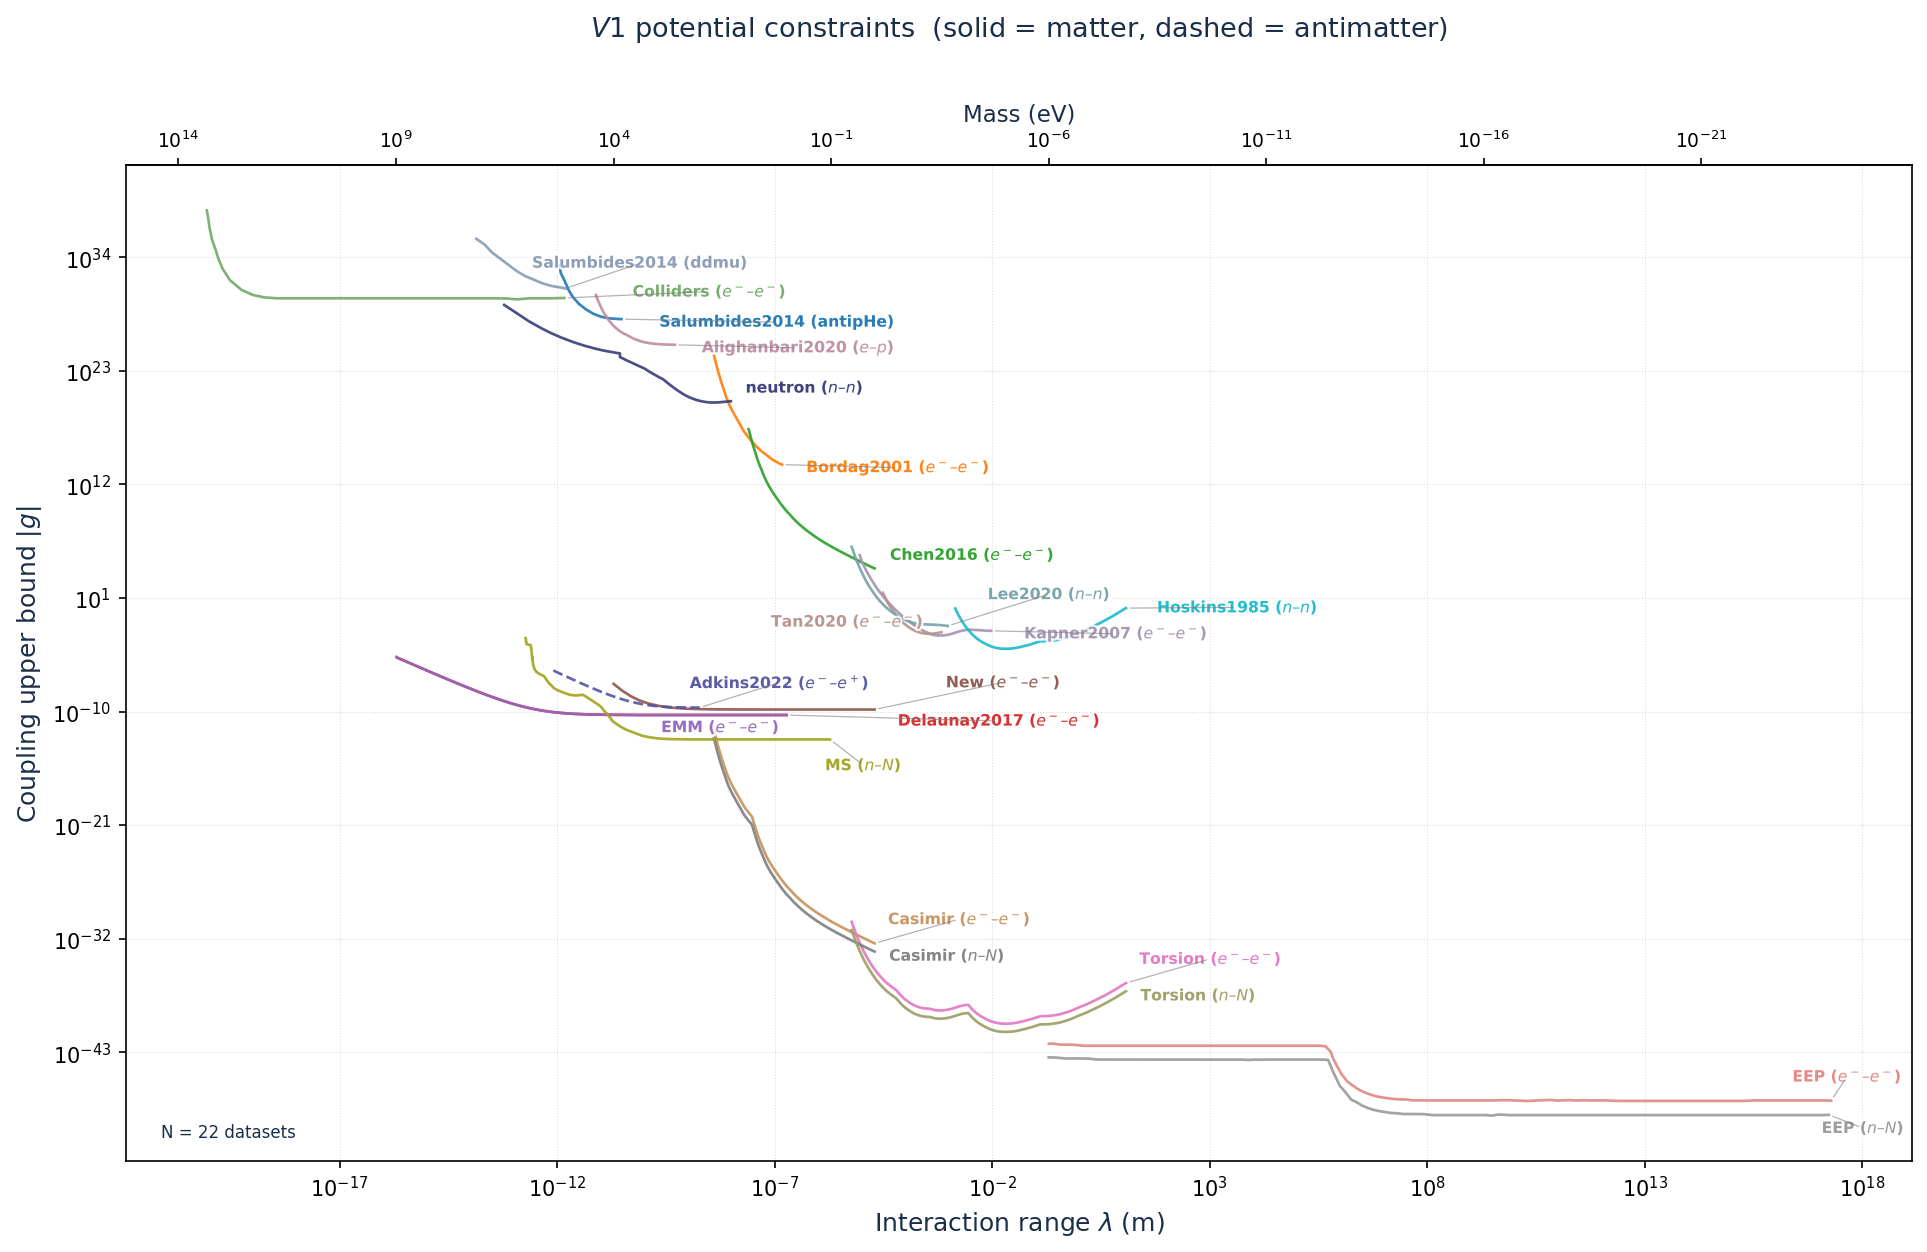
\includegraphics[width=0.85\textwidth,height=0.9\textheight,keepaspectratio]{constraint_V1.png}
\caption{Constraint atlas for $V_1$.}
\label{fig:atlas-v1}
\end{figure}
\clearpage

\begin{figure}[p]
\centering
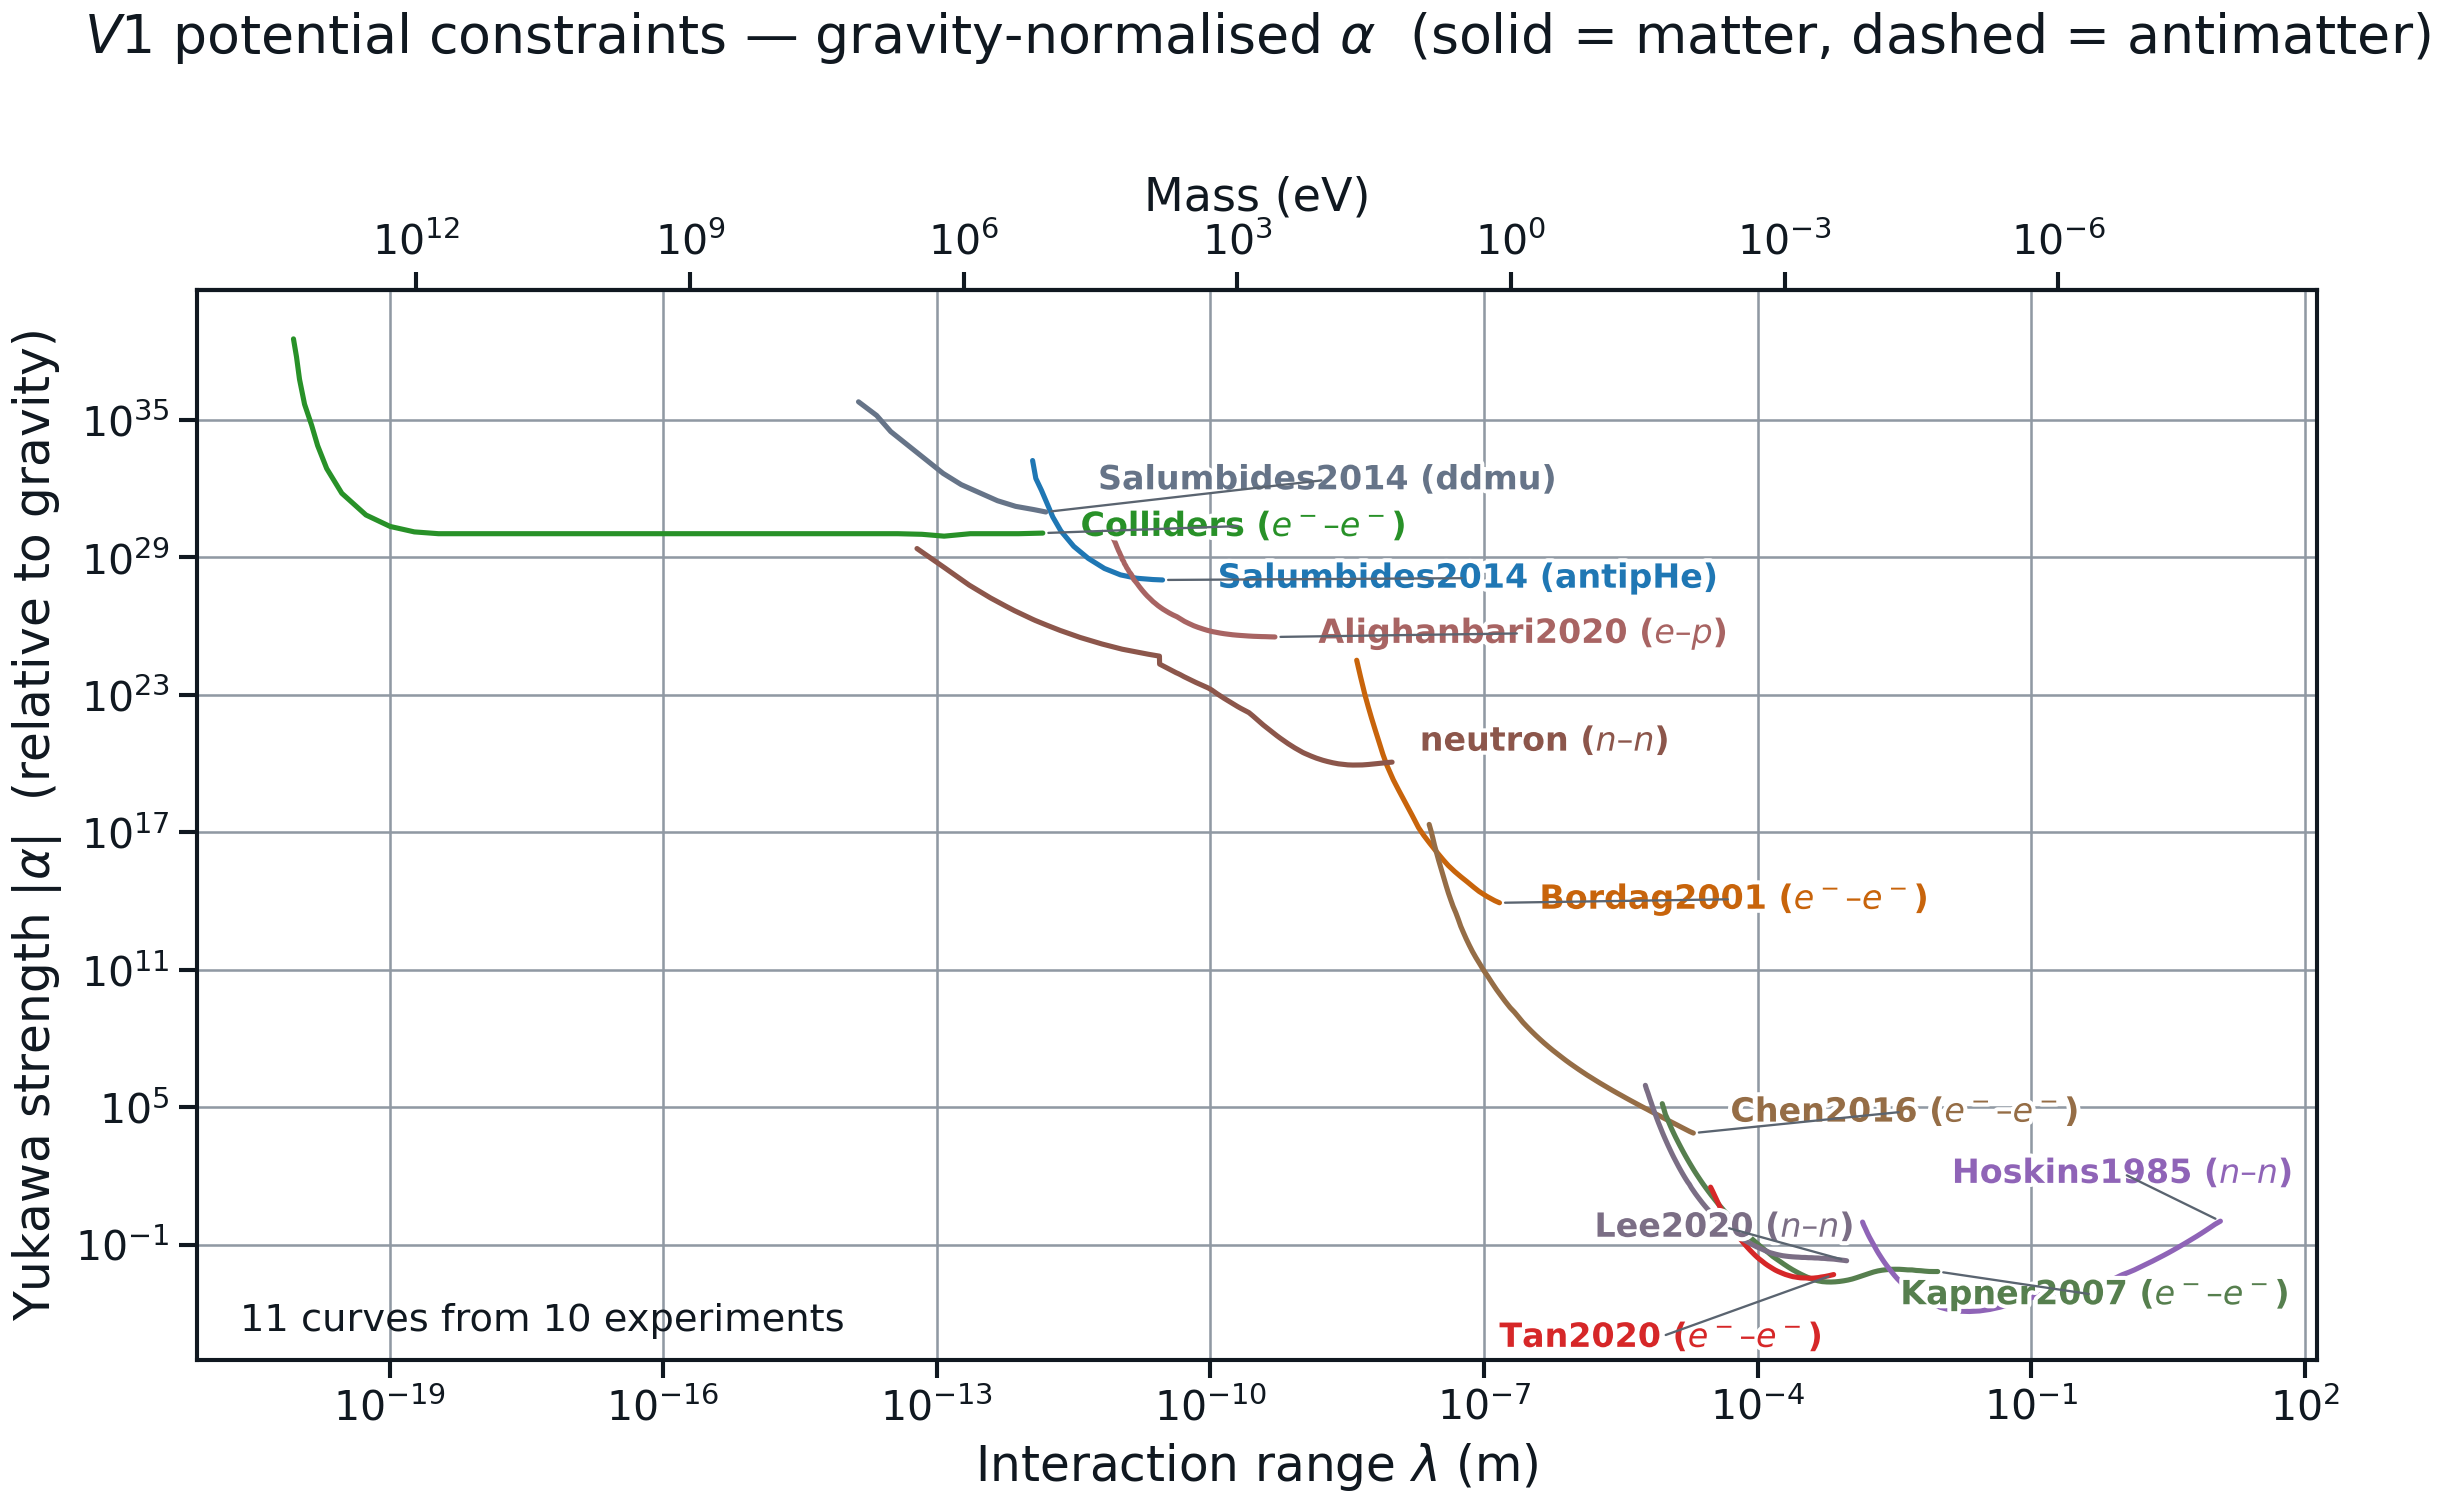
\includegraphics[width=0.85\textwidth,height=0.9\textheight,keepaspectratio]{constraint_V1_alpha.png}
\caption{Constraint atlas for $V_1$, gravity-normalised. These bounds are
published as the Yukawa strength $|\alpha|$ relative to gravity rather than
as a coupling $|g|$, and are shown on a separate axis because the two
conventions typically differ by more than thirty orders of magnitude.}
\label{fig:atlas-v1-alpha}
\end{figure}
\clearpage

\begin{figure}[p]
\centering
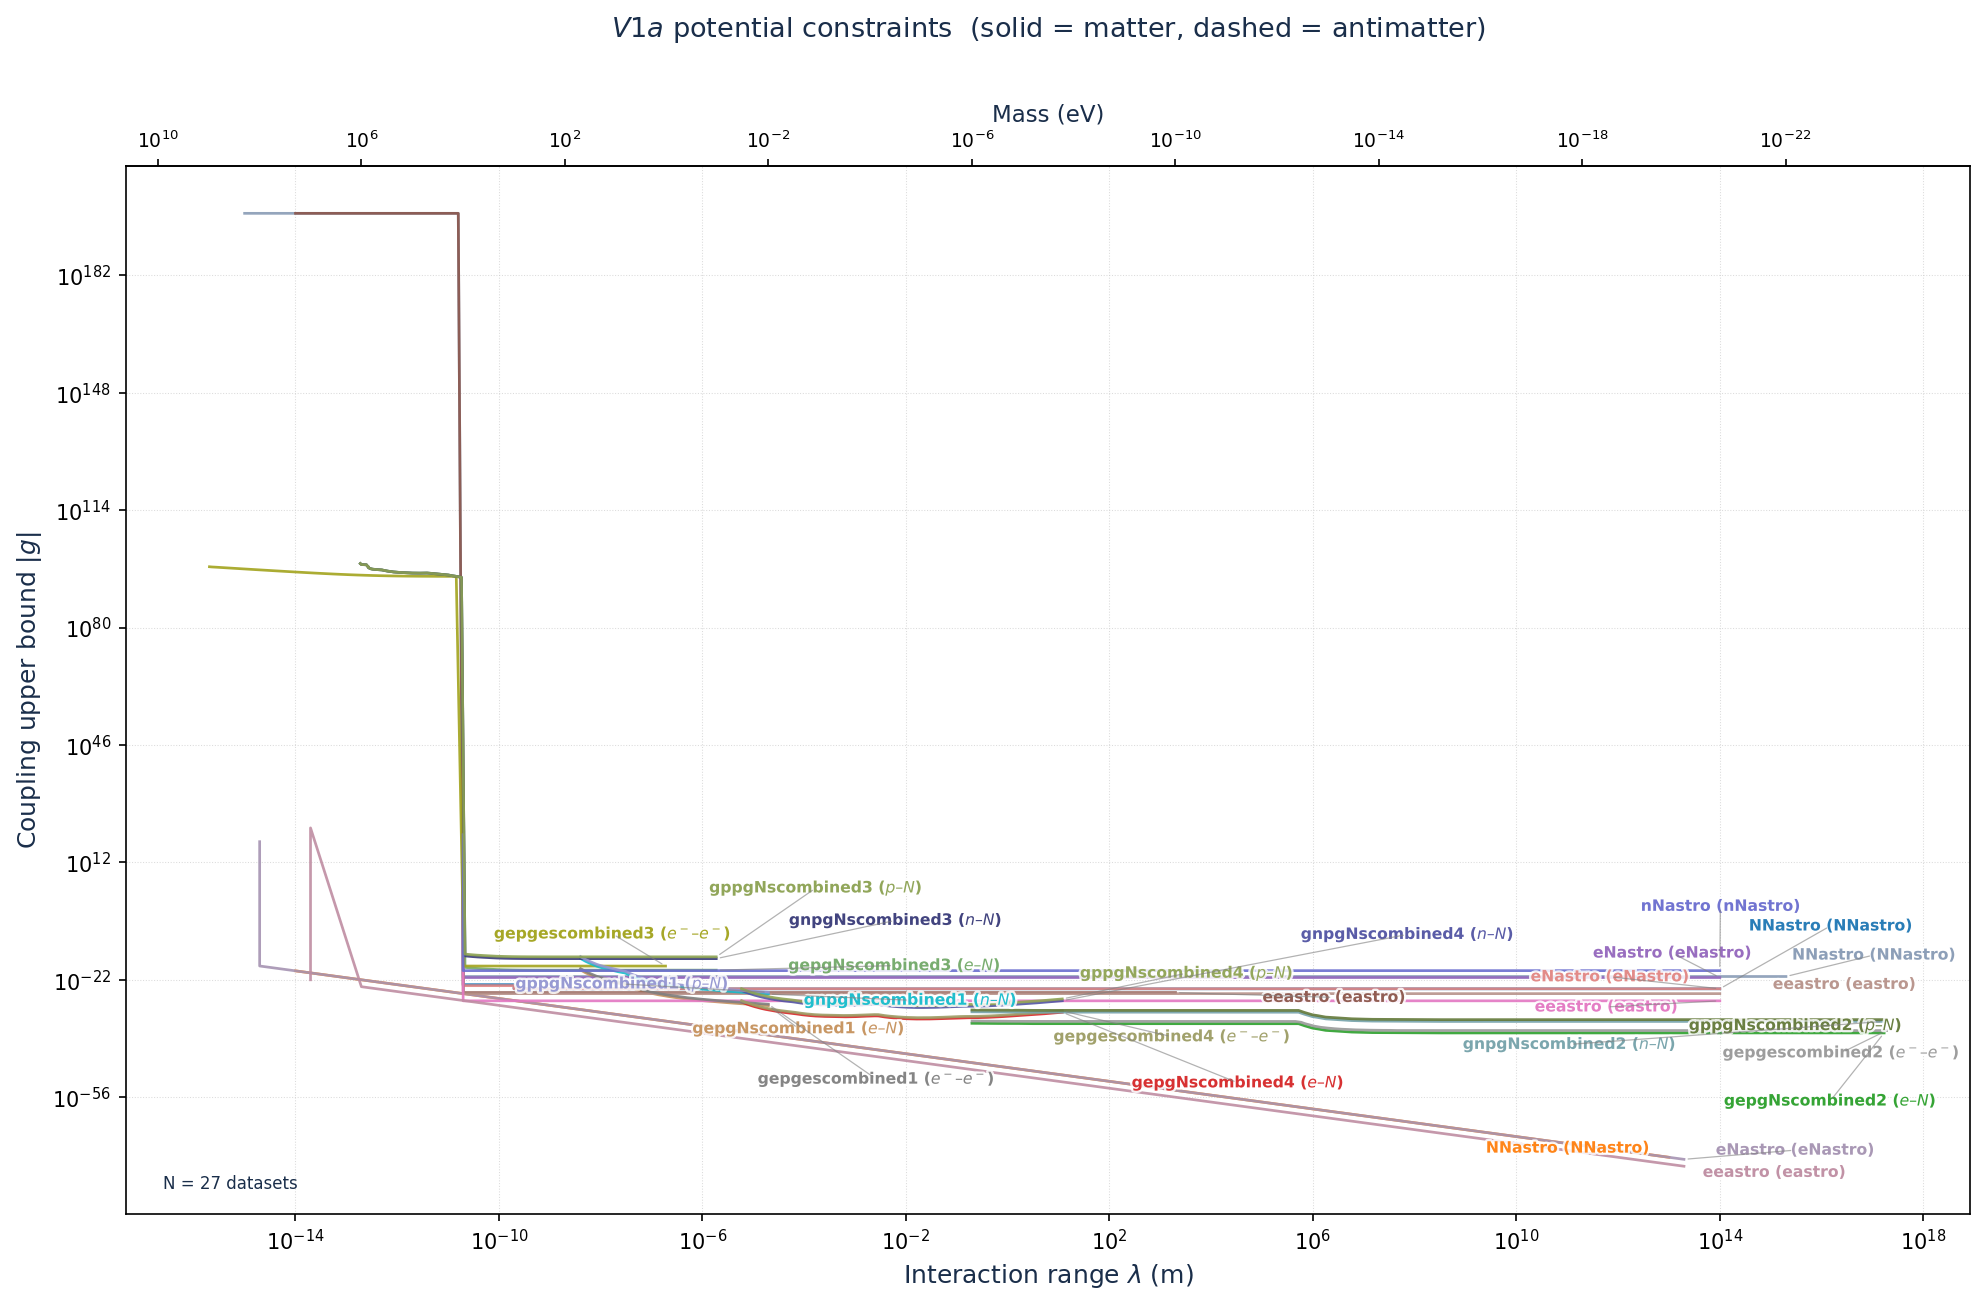
\includegraphics[width=0.85\textwidth,height=0.9\textheight,keepaspectratio]{constraint_V1a.png}
\caption{Constraint atlas for $V_{1a}$.}
\label{fig:atlas-v1a}
\end{figure}
\clearpage

\begin{figure}[p]
\centering
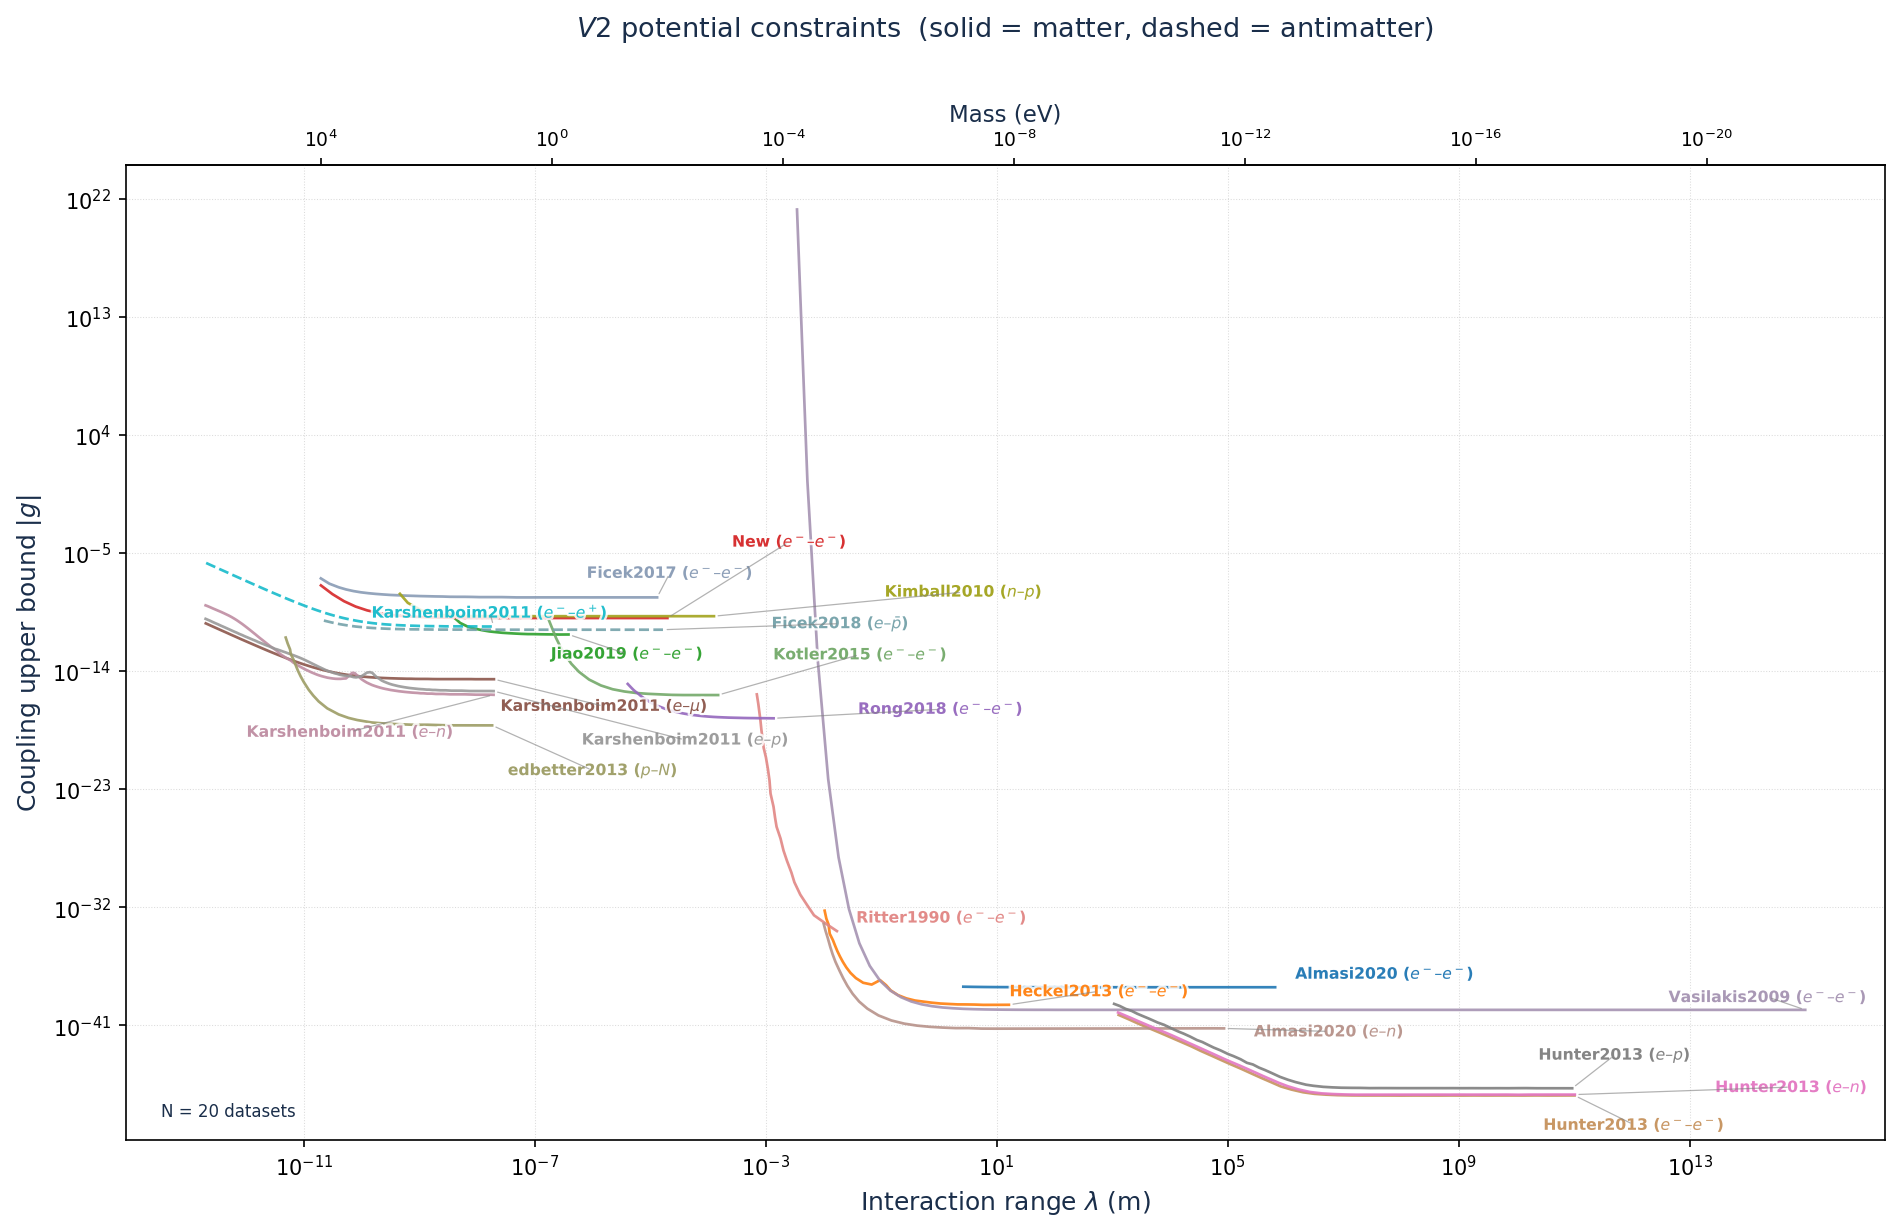
\includegraphics[width=0.85\textwidth,height=0.9\textheight,keepaspectratio]{constraint_V2.png}
\caption{Constraint atlas for $V_2$.}
\label{fig:atlas-v2}
\end{figure}
\clearpage

\begin{figure}[p]
\centering
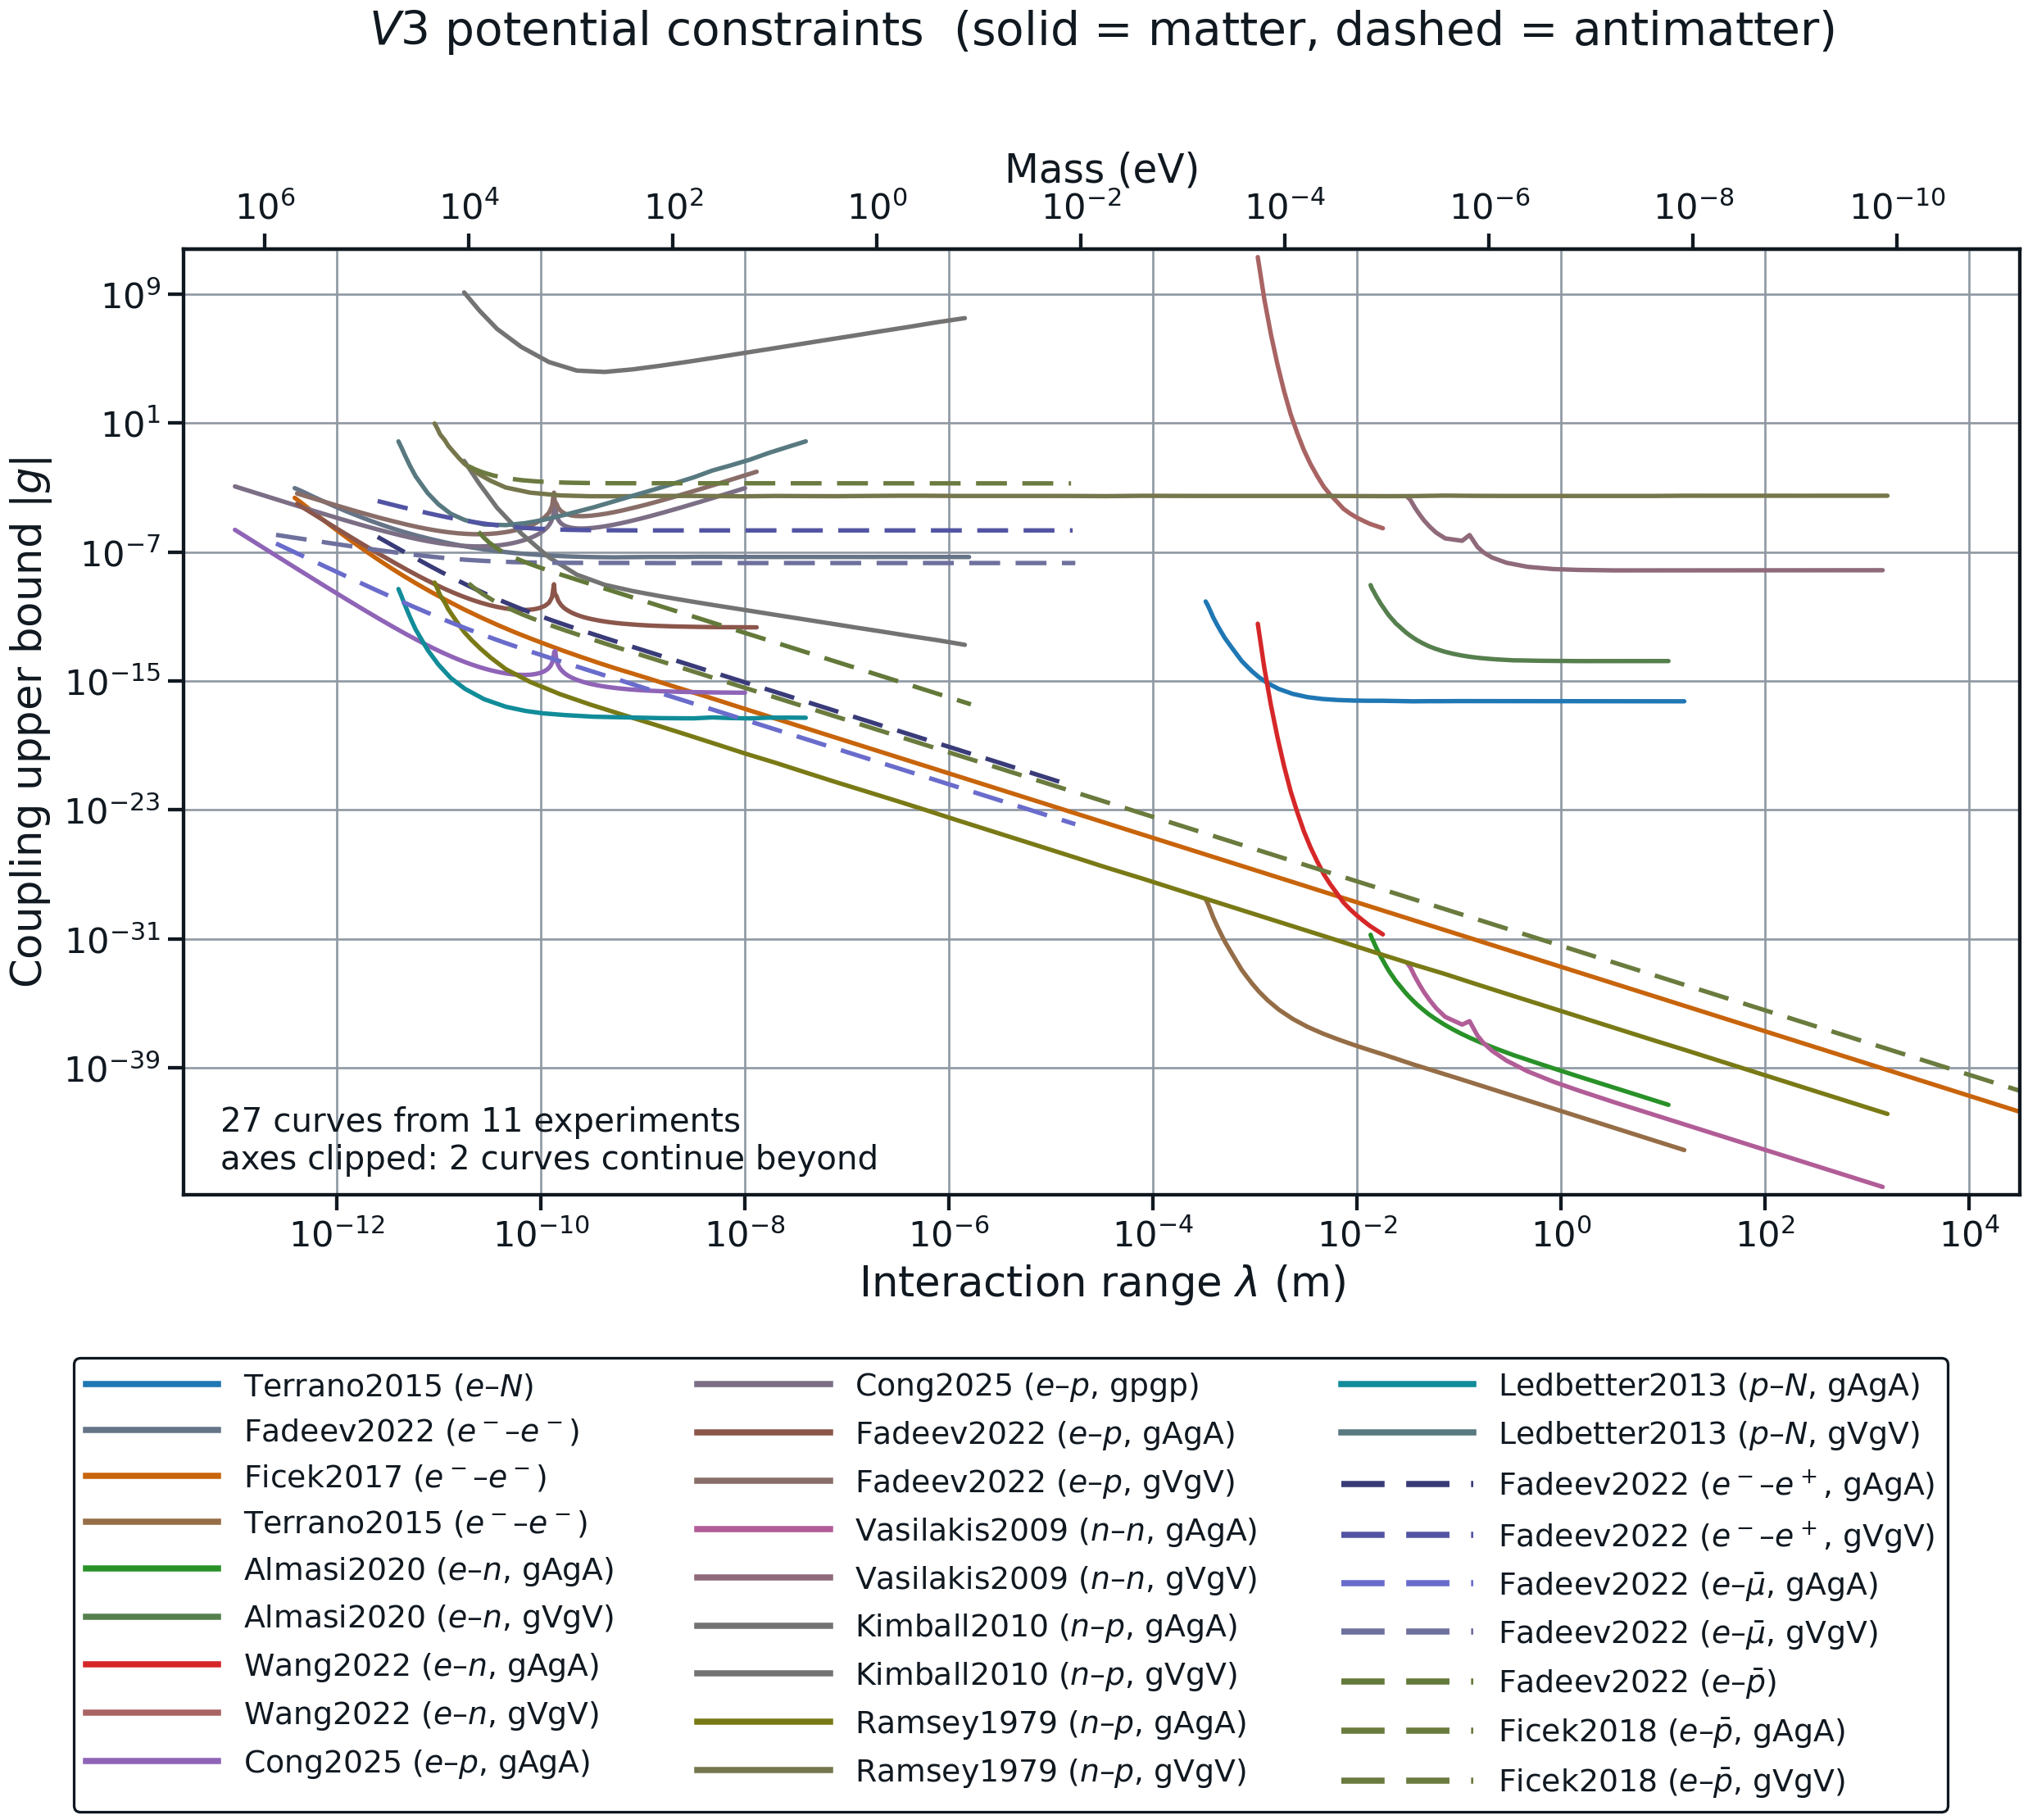
\includegraphics[width=0.85\textwidth,height=0.9\textheight,keepaspectratio]{constraint_V3.png}
\caption{Constraint atlas for $V_3$, the best-covered potential in the
antimatter sector (39 datasets, 10 of them antimatter).}
\label{fig:atlas-v3}
\end{figure}
\clearpage

\begin{figure}[p]
\centering
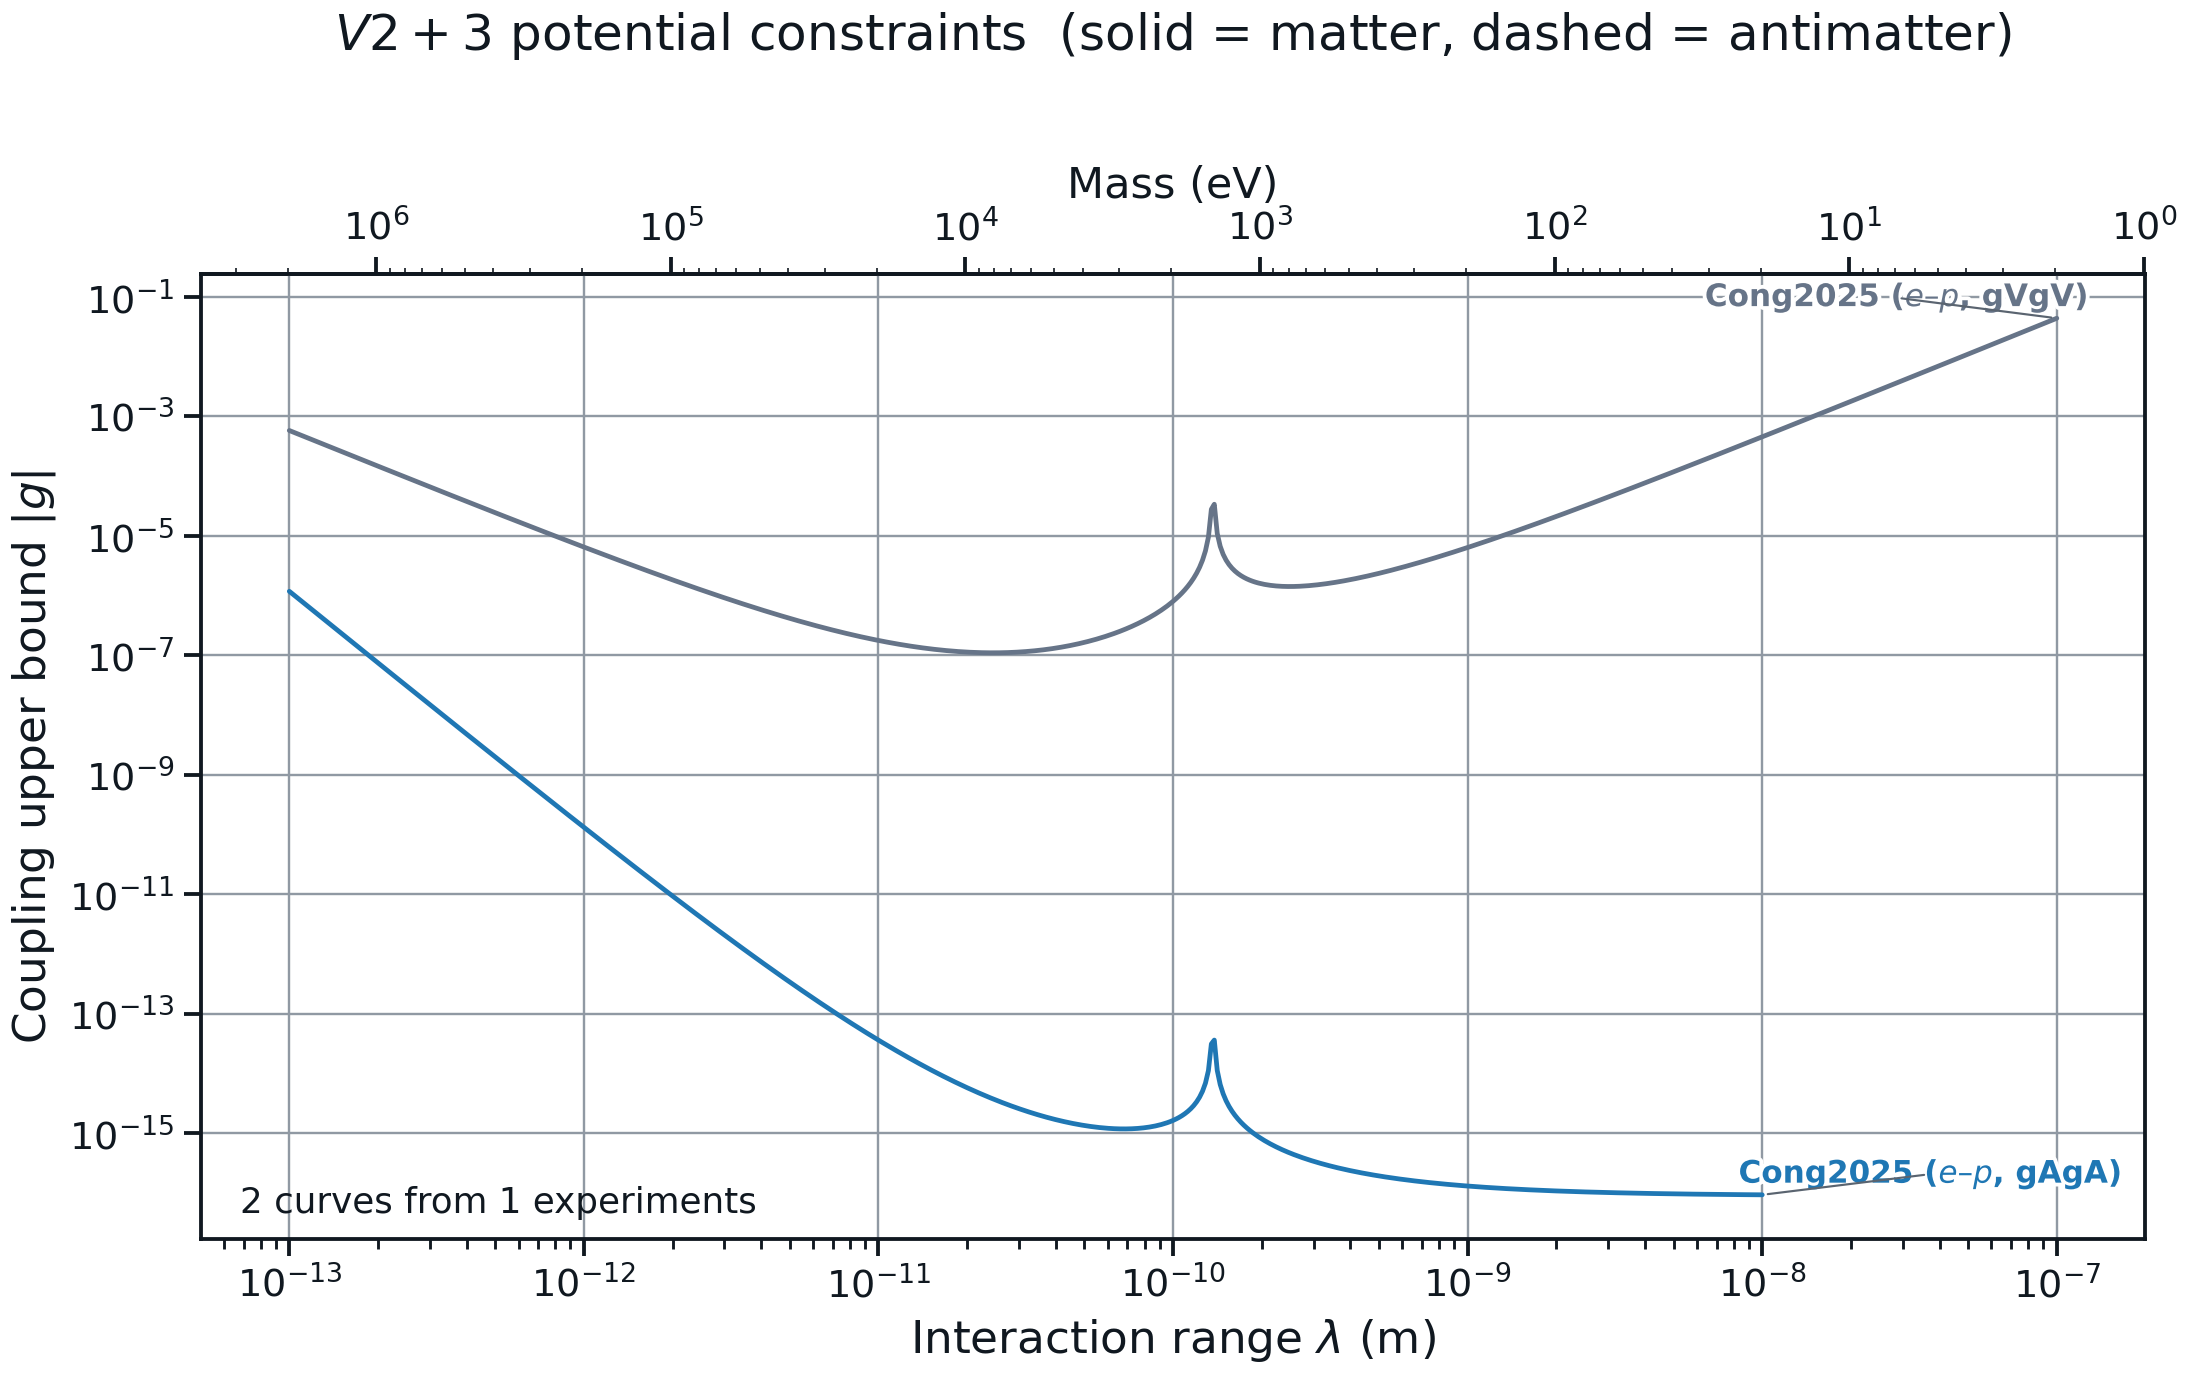
\includegraphics[width=0.85\textwidth,height=0.9\textheight,keepaspectratio]{constraint_V2+3.png}
\caption{Constraint atlas for $V_{2+3}$. Only two datasets carry this
combination label, both matter-sector; the great majority of what earlier
drafts filed under $V_{2+3}$ are $V_3$-only bounds and appear in
Figure~\ref{fig:atlas-v3}.}
\label{fig:atlas-v23}
\end{figure}
\clearpage

\begin{figure}[p]
\centering
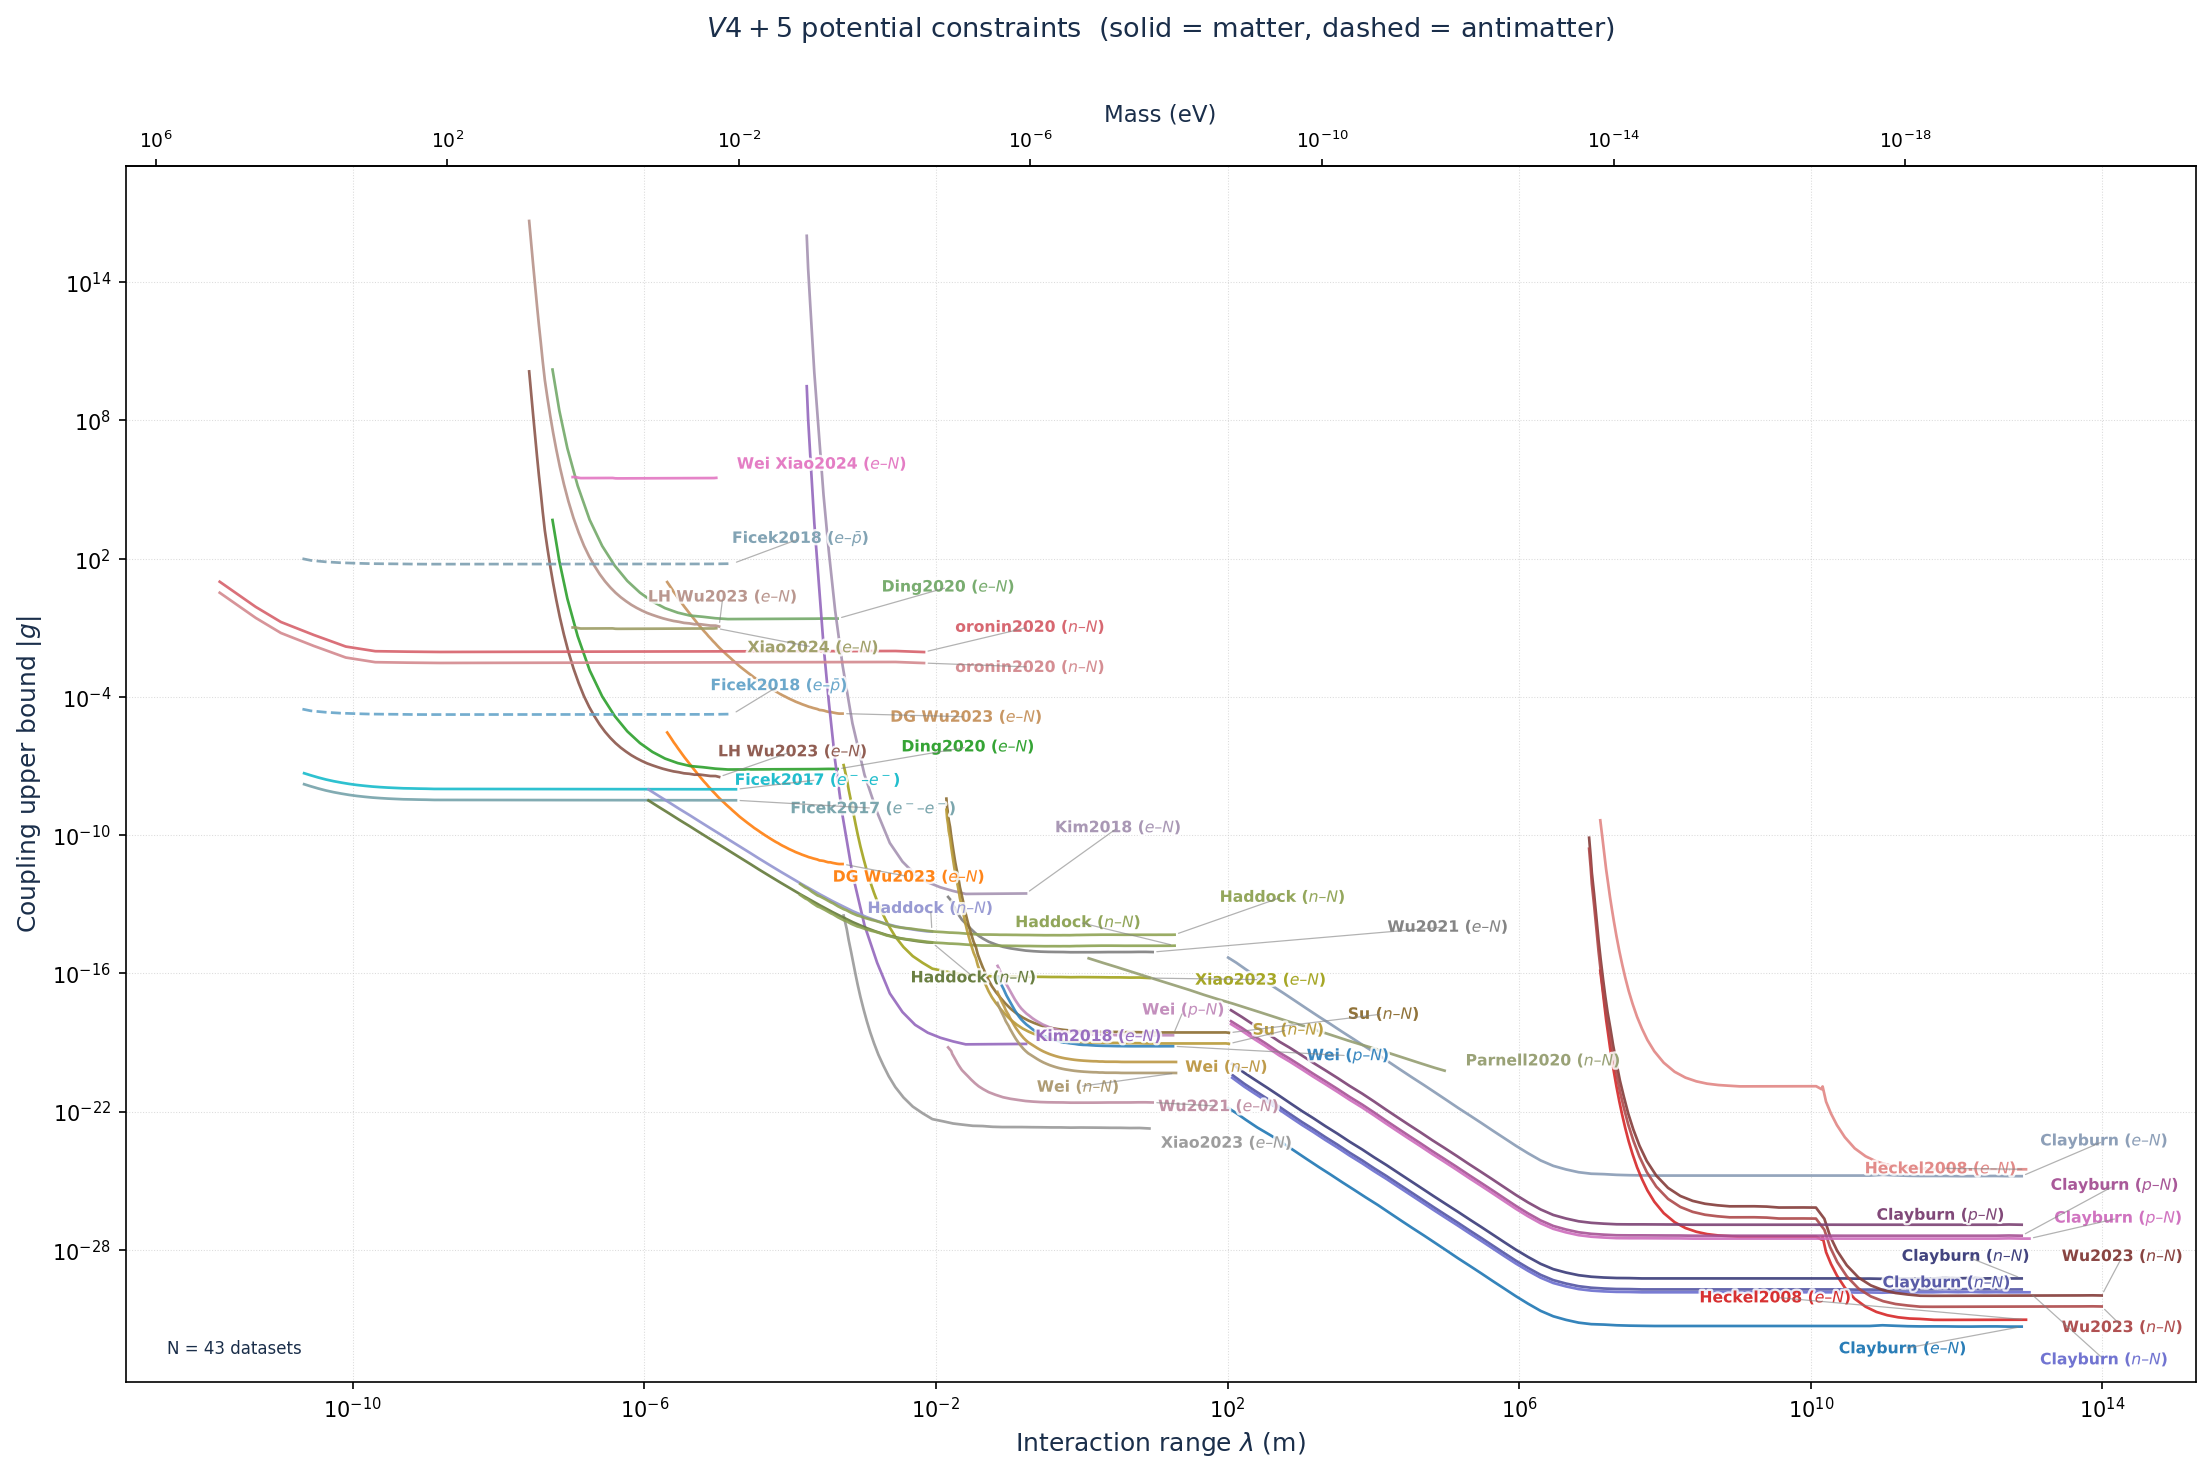
\includegraphics[width=0.85\textwidth,height=0.9\textheight,keepaspectratio]{constraint_V4+5.png}
\caption{Constraint atlas for $V_{4+5}$, the most populated potential in the database (61 datasets).}
\label{fig:atlas-v45}
\end{figure}
\clearpage

\begin{figure}[p]
\centering
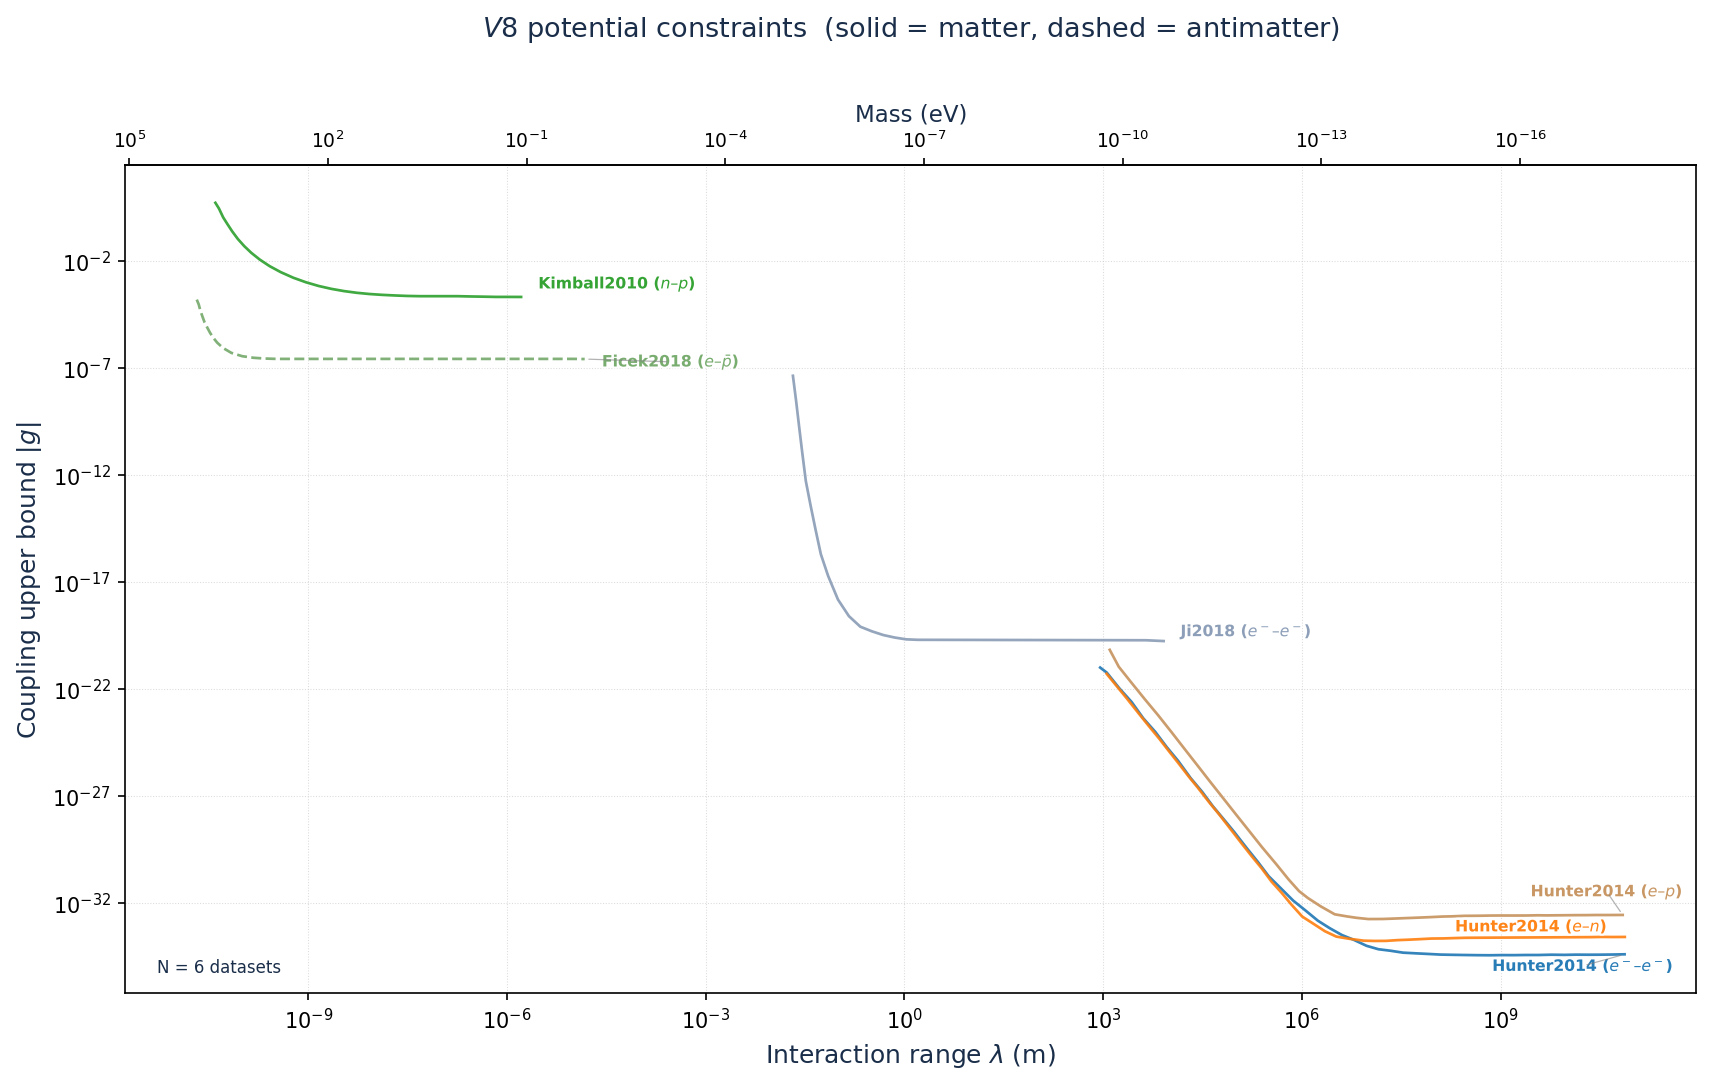
\includegraphics[width=0.85\textwidth,height=0.9\textheight,keepaspectratio]{constraint_V8.png}
\caption{Constraint atlas for $V_8$.}
\label{fig:atlas-v8}
\end{figure}
\clearpage

\begin{figure}[p]
\centering
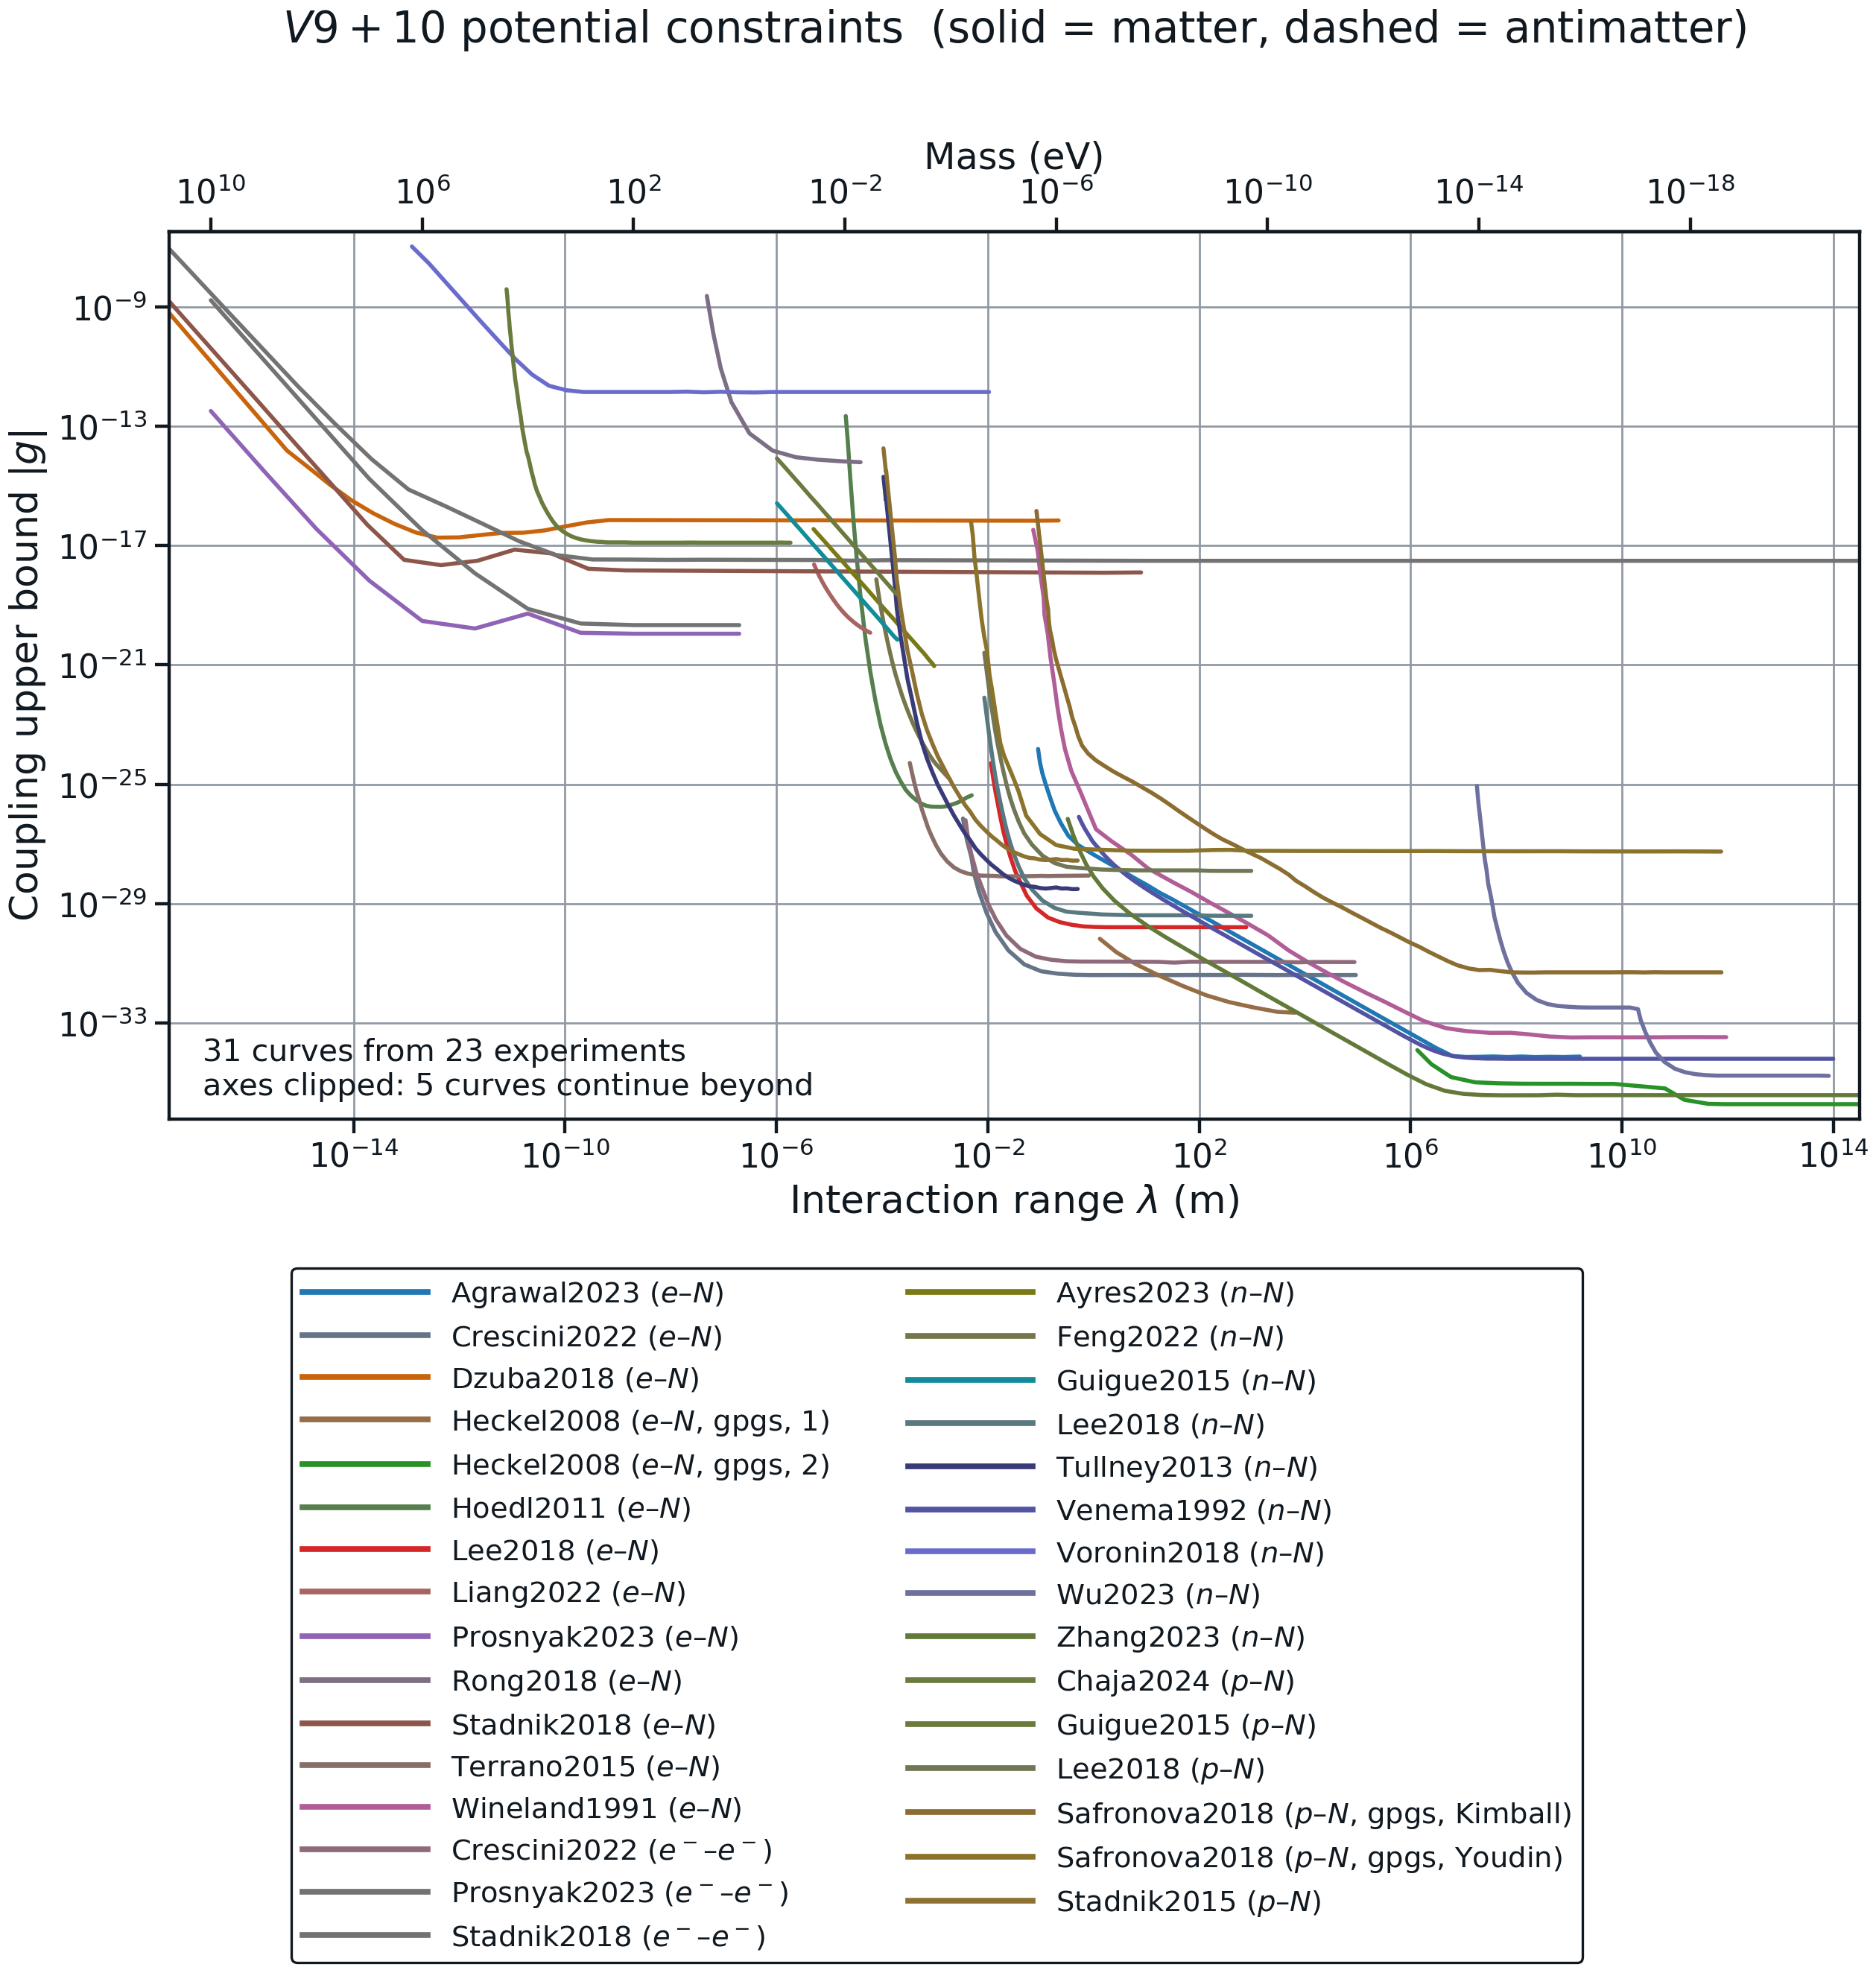
\includegraphics[width=0.85\textwidth,height=0.9\textheight,keepaspectratio]{constraint_V9+10.png}
\caption{Constraint atlas for $V_{9+10}$.}
\label{fig:atlas-v910}
\end{figure}
\clearpage

\begin{figure}[p]
\centering
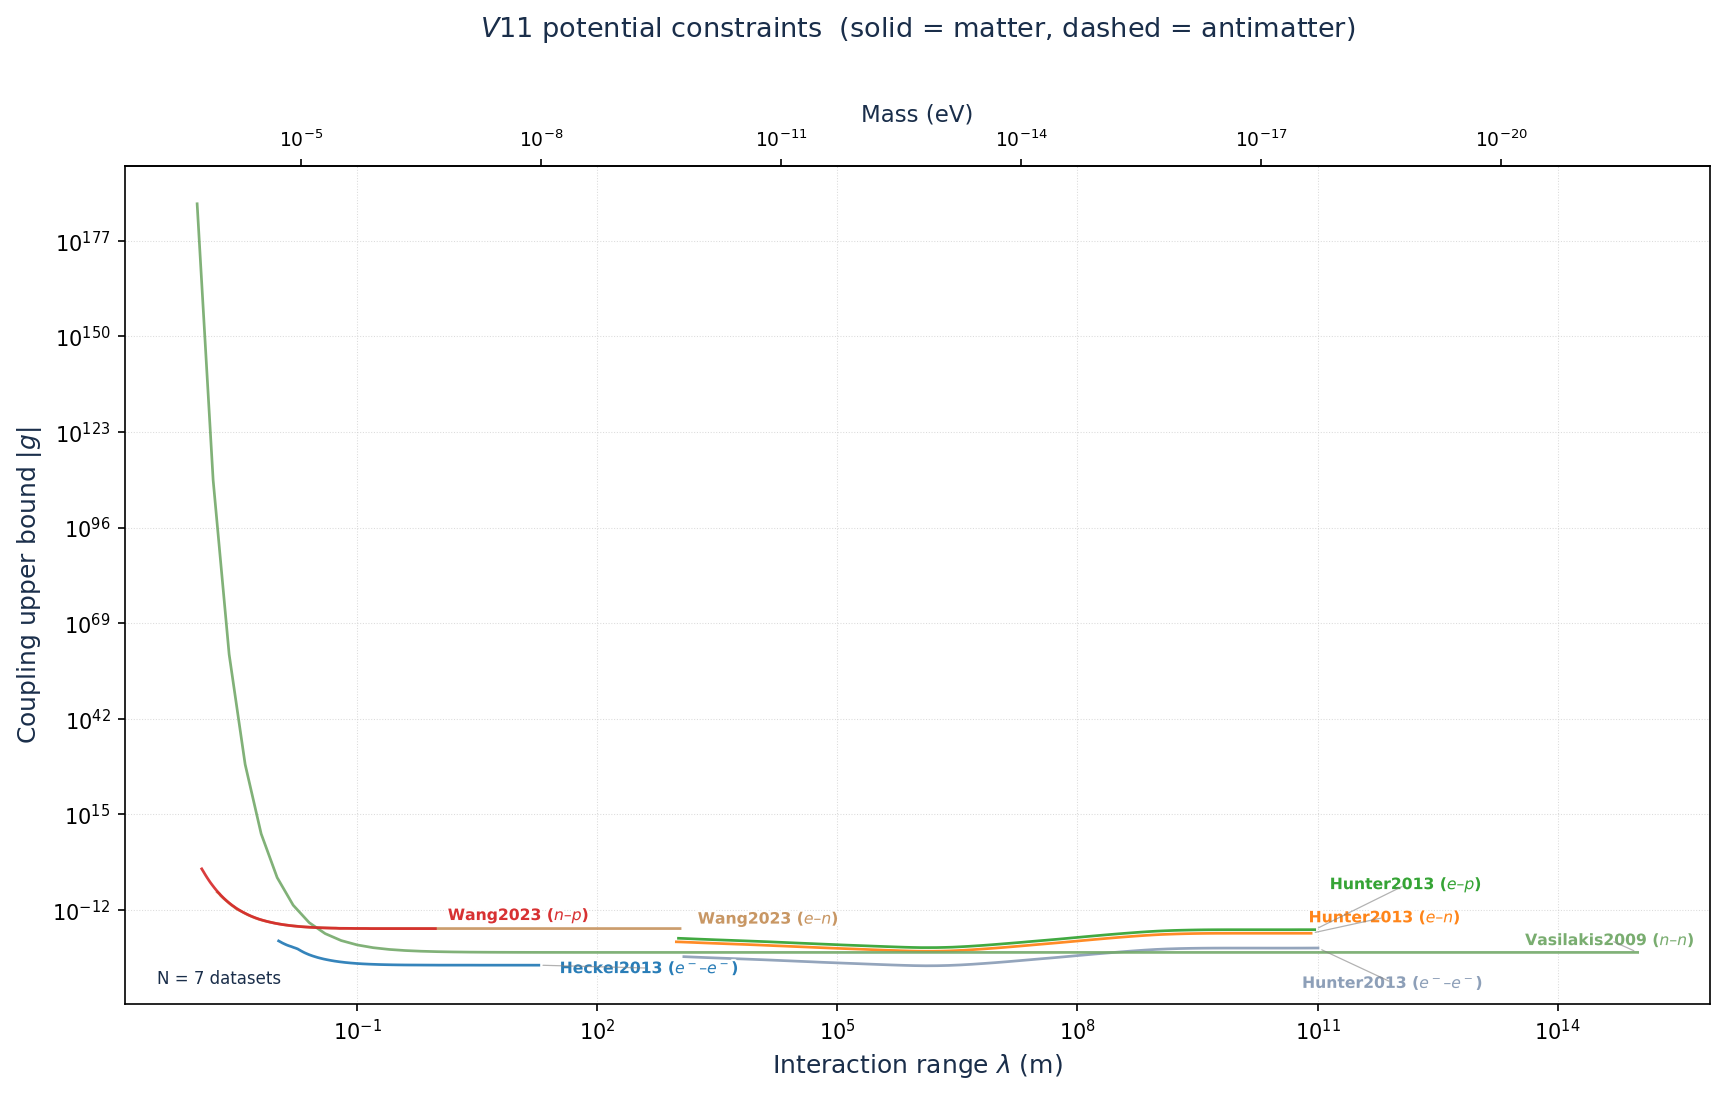
\includegraphics[width=0.85\textwidth,height=0.9\textheight,keepaspectratio]{constraint_V11.png}
\caption{Constraint atlas for $V_{11}$.}
\label{fig:atlas-v11}
\end{figure}
\clearpage

\begin{figure}[p]
\centering
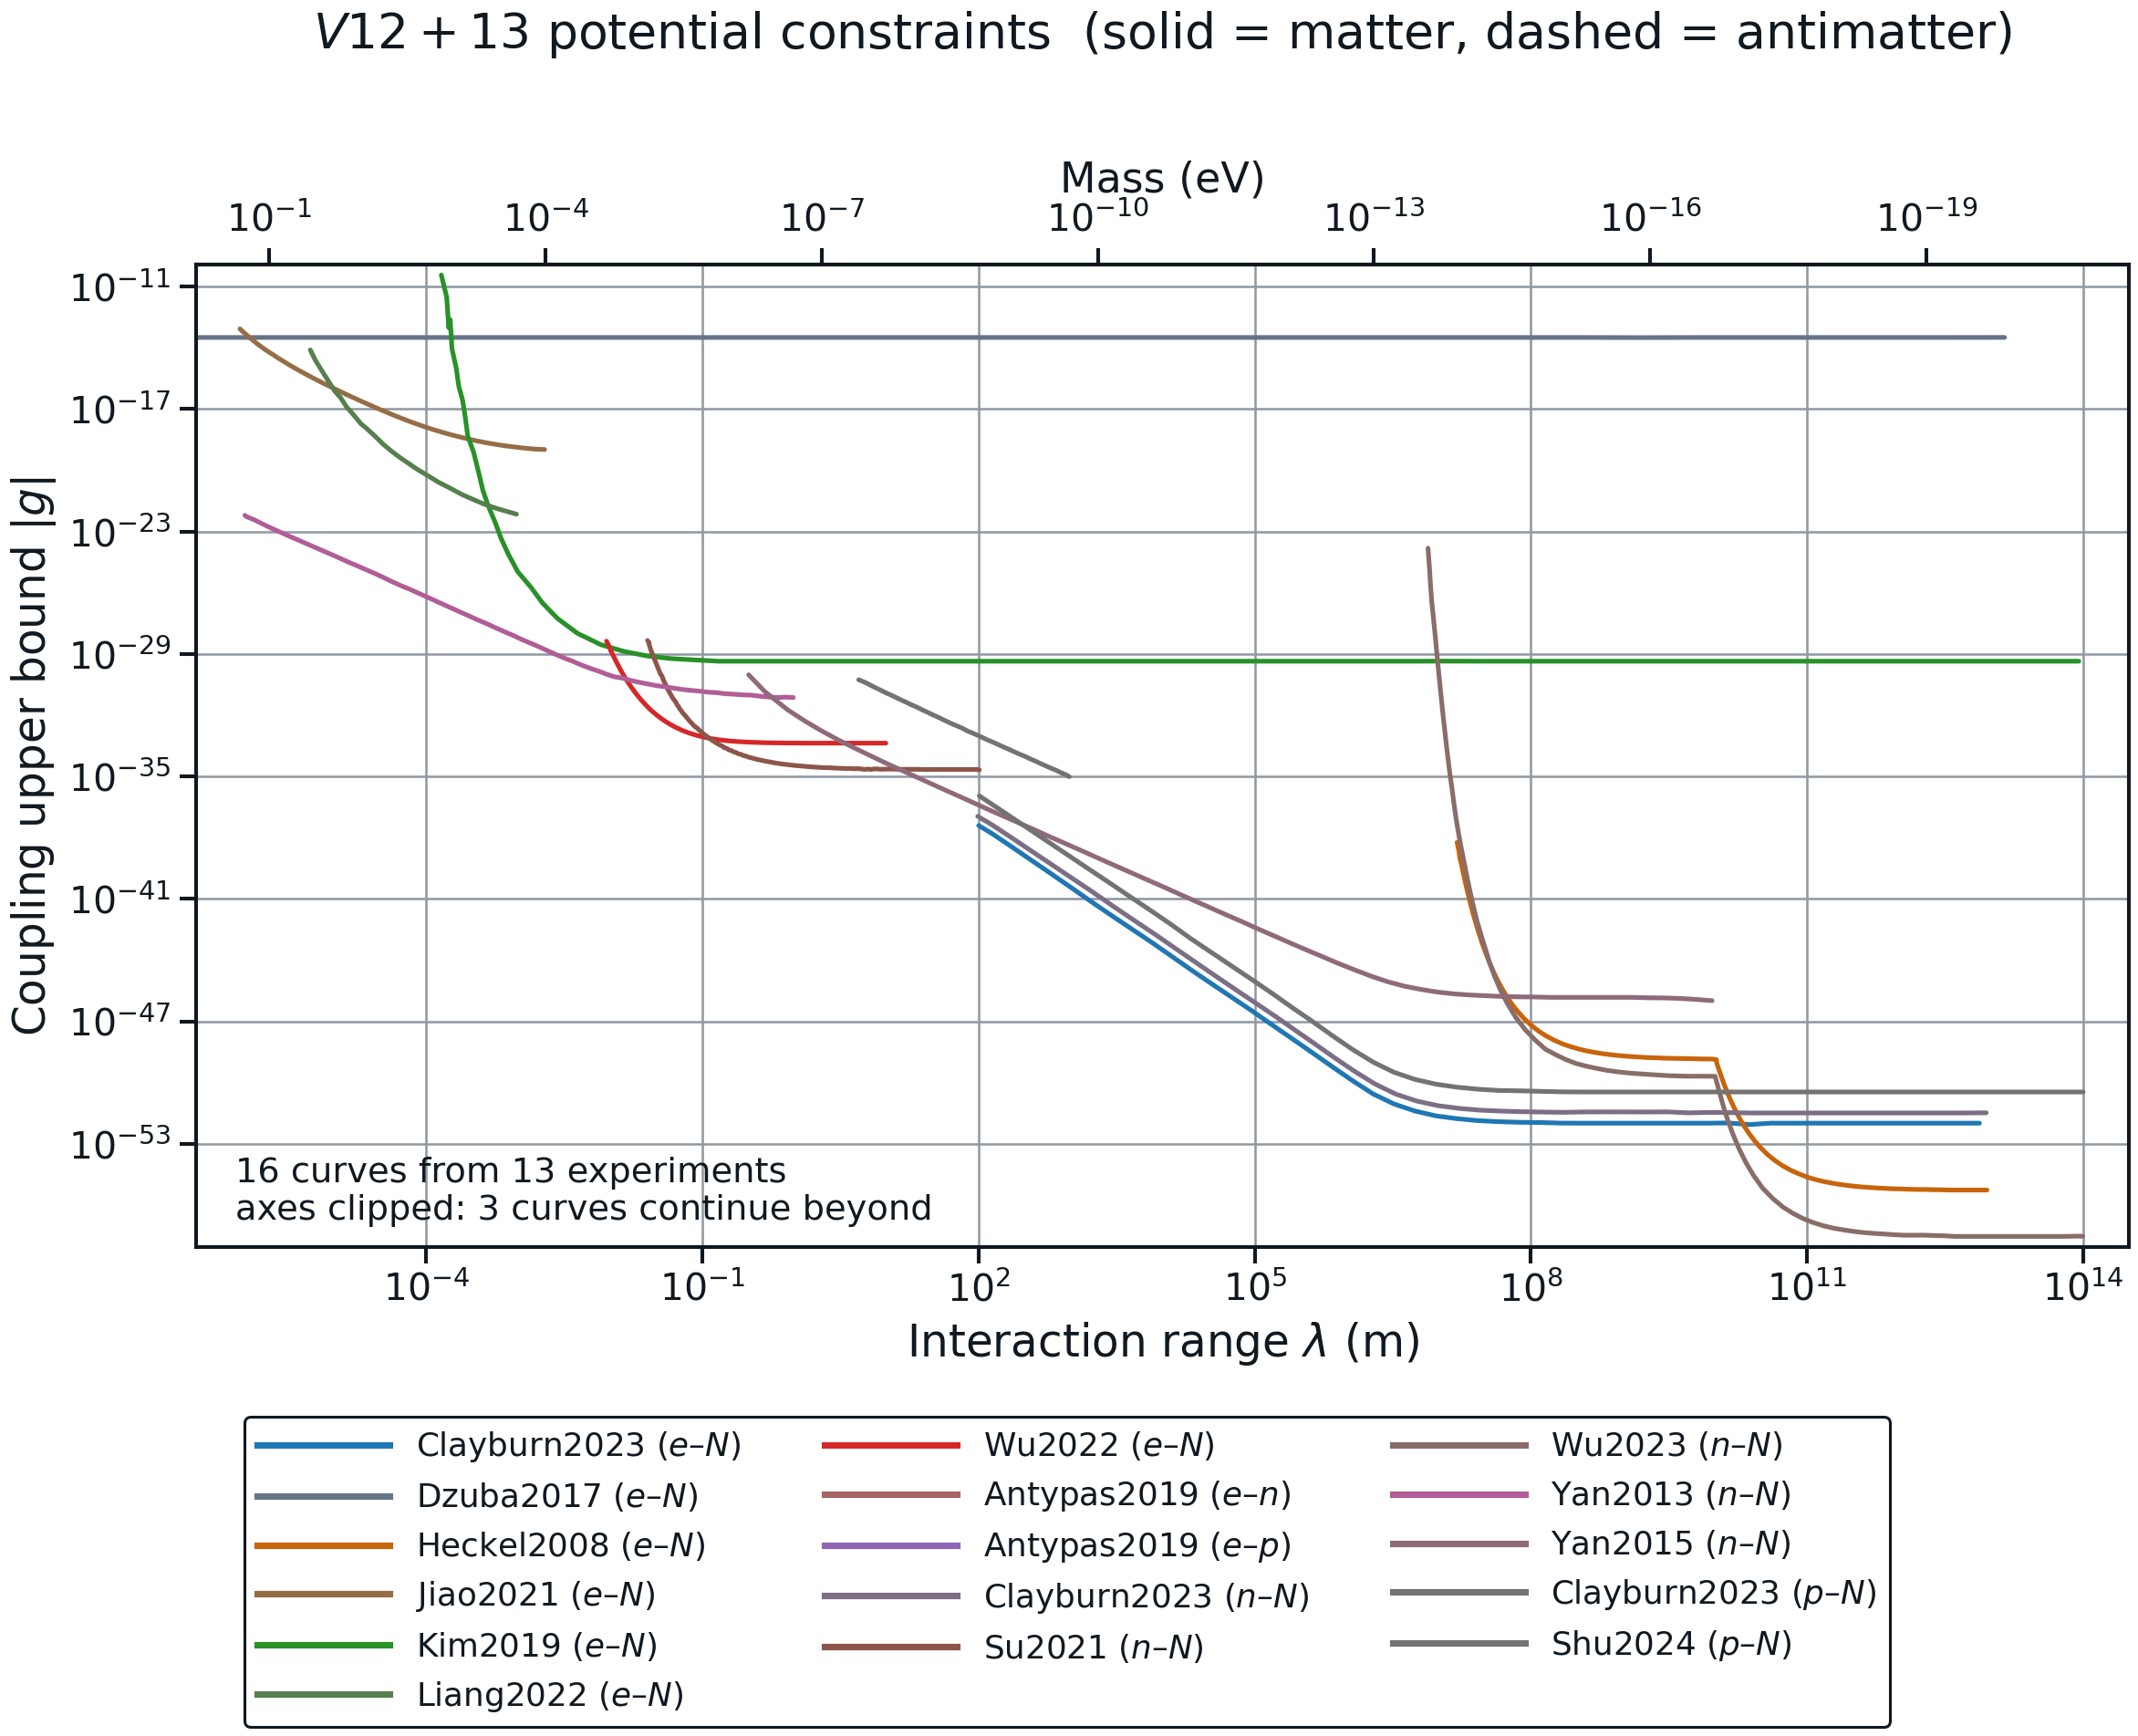
\includegraphics[width=0.85\textwidth,height=0.9\textheight,keepaspectratio]{constraint_V12+13.png}
\caption{Constraint atlas for $V_{12+13}$.}
\label{fig:atlas-v1213}
\end{figure}
\clearpage

\begin{figure}[p]
\centering
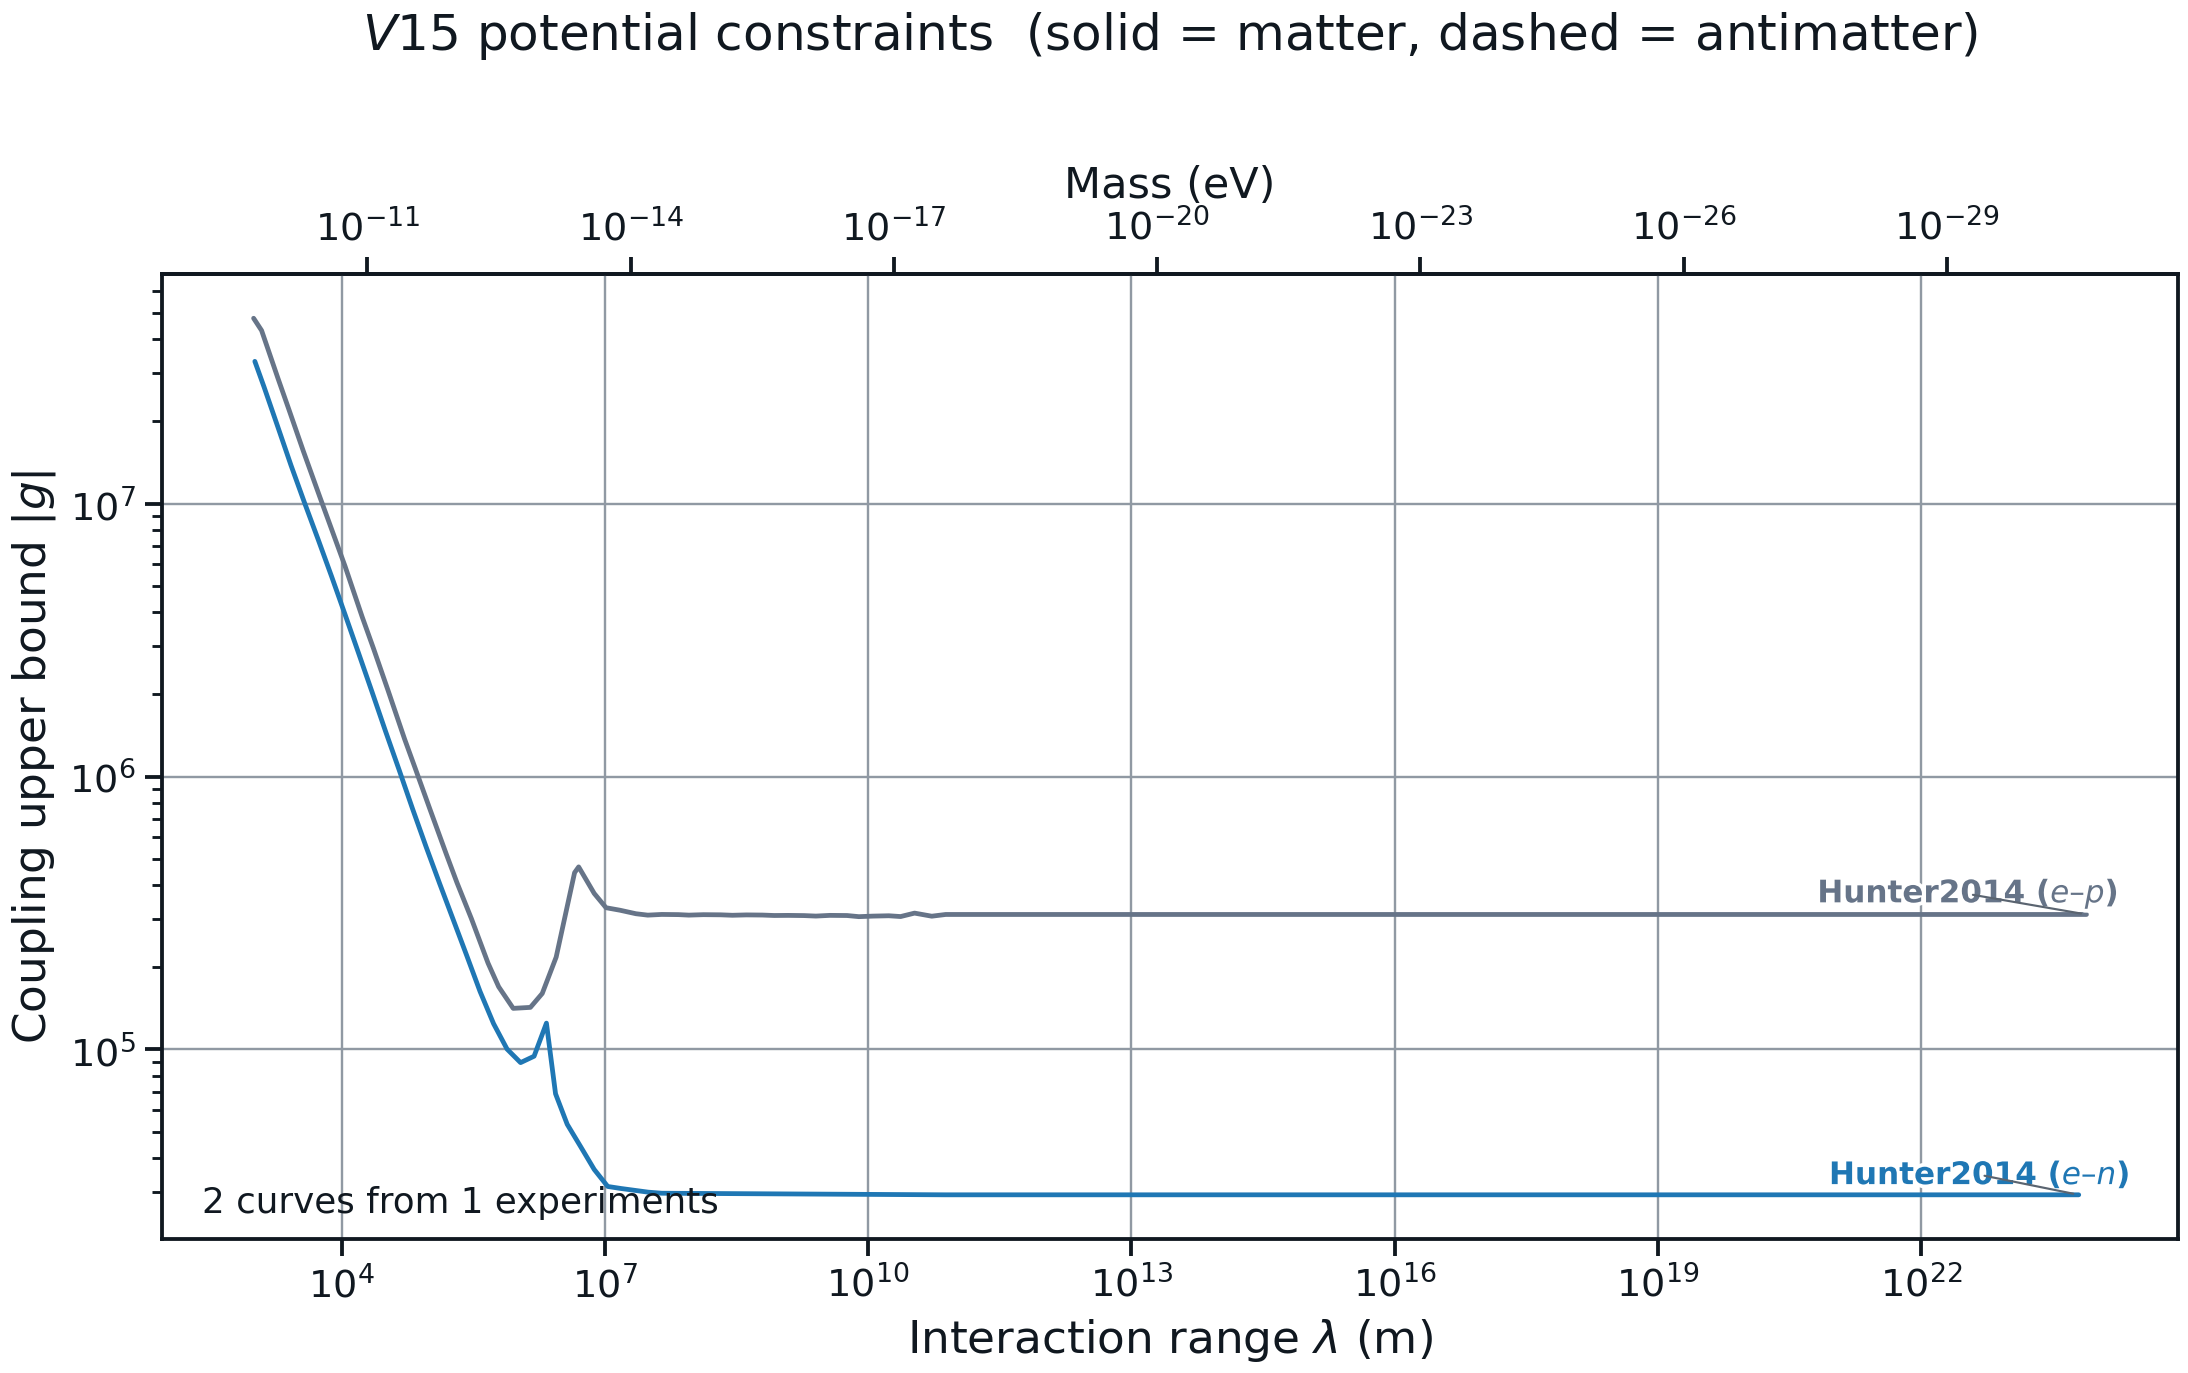
\includegraphics[width=0.85\textwidth,height=0.9\textheight,keepaspectratio]{constraint_V15.png}
\caption{Constraint atlas for $V_{15}$.}
\label{fig:atlas-v15}
\end{figure}
\clearpage

\begin{figure}[p]
\centering
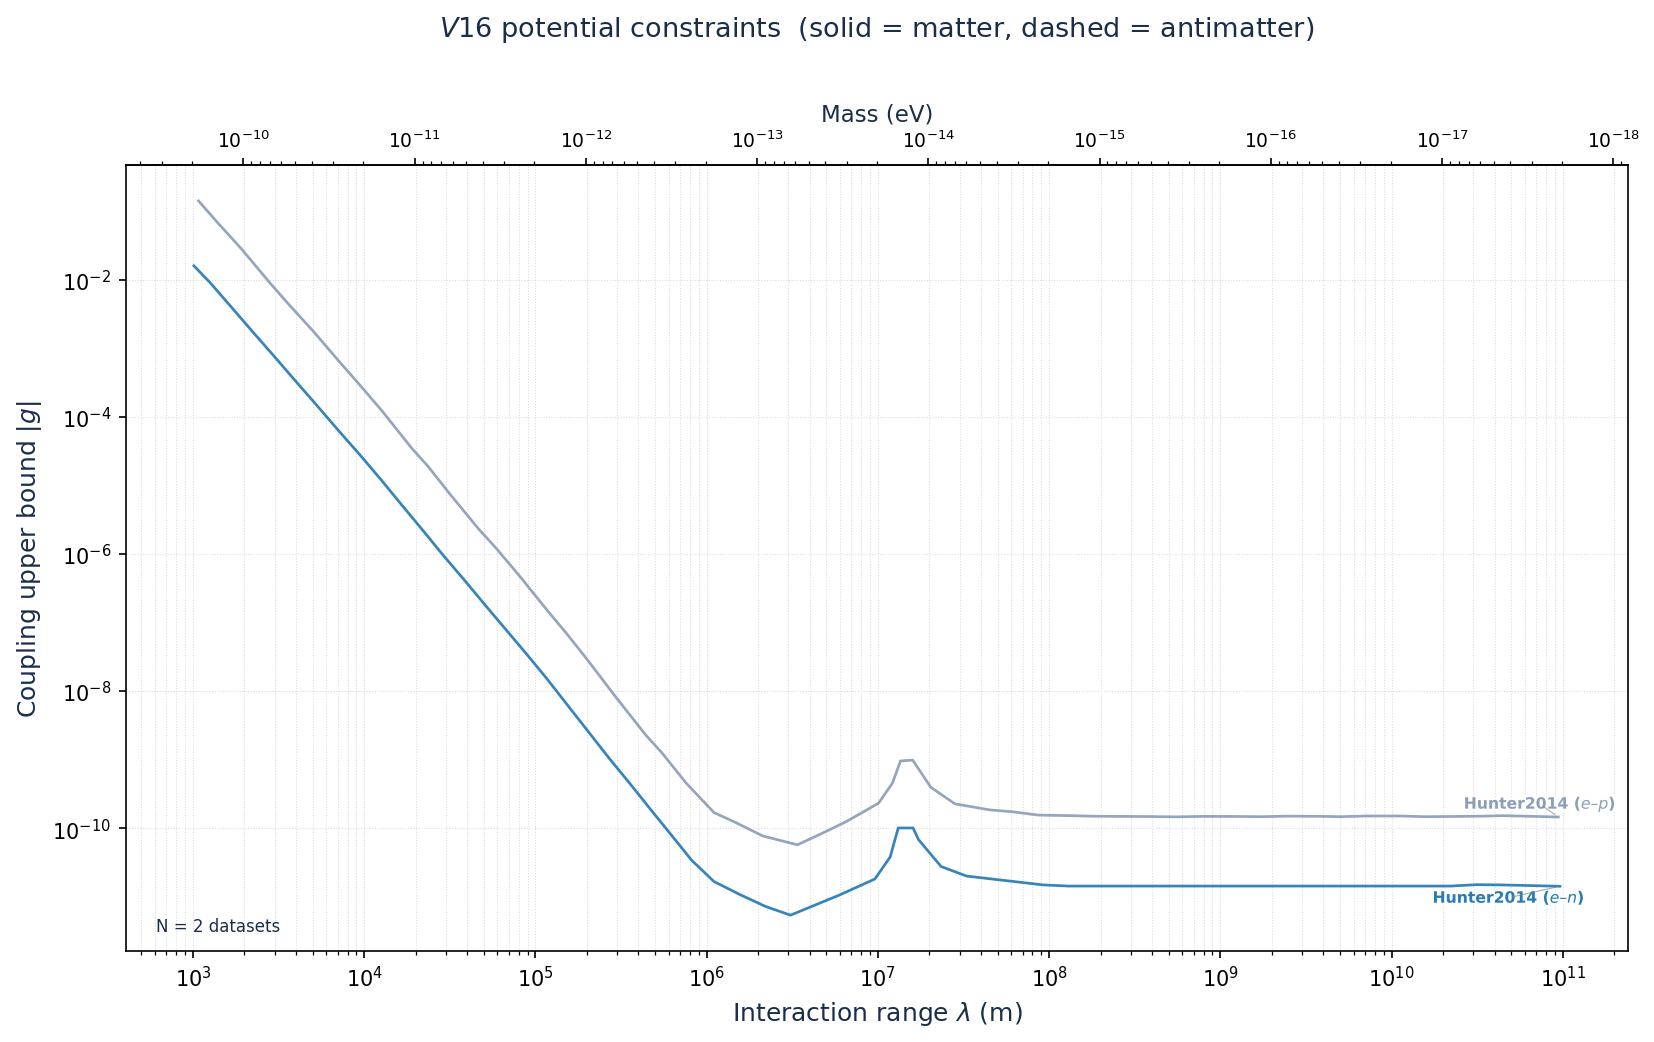
\includegraphics[width=0.85\textwidth,height=0.9\textheight,keepaspectratio]{constraint_V16.png}
\caption{Constraint atlas for $V_{16}$.}
\label{fig:atlas-v16}
\end{figure}
\clearpage

\begin{figure}[p]
\centering
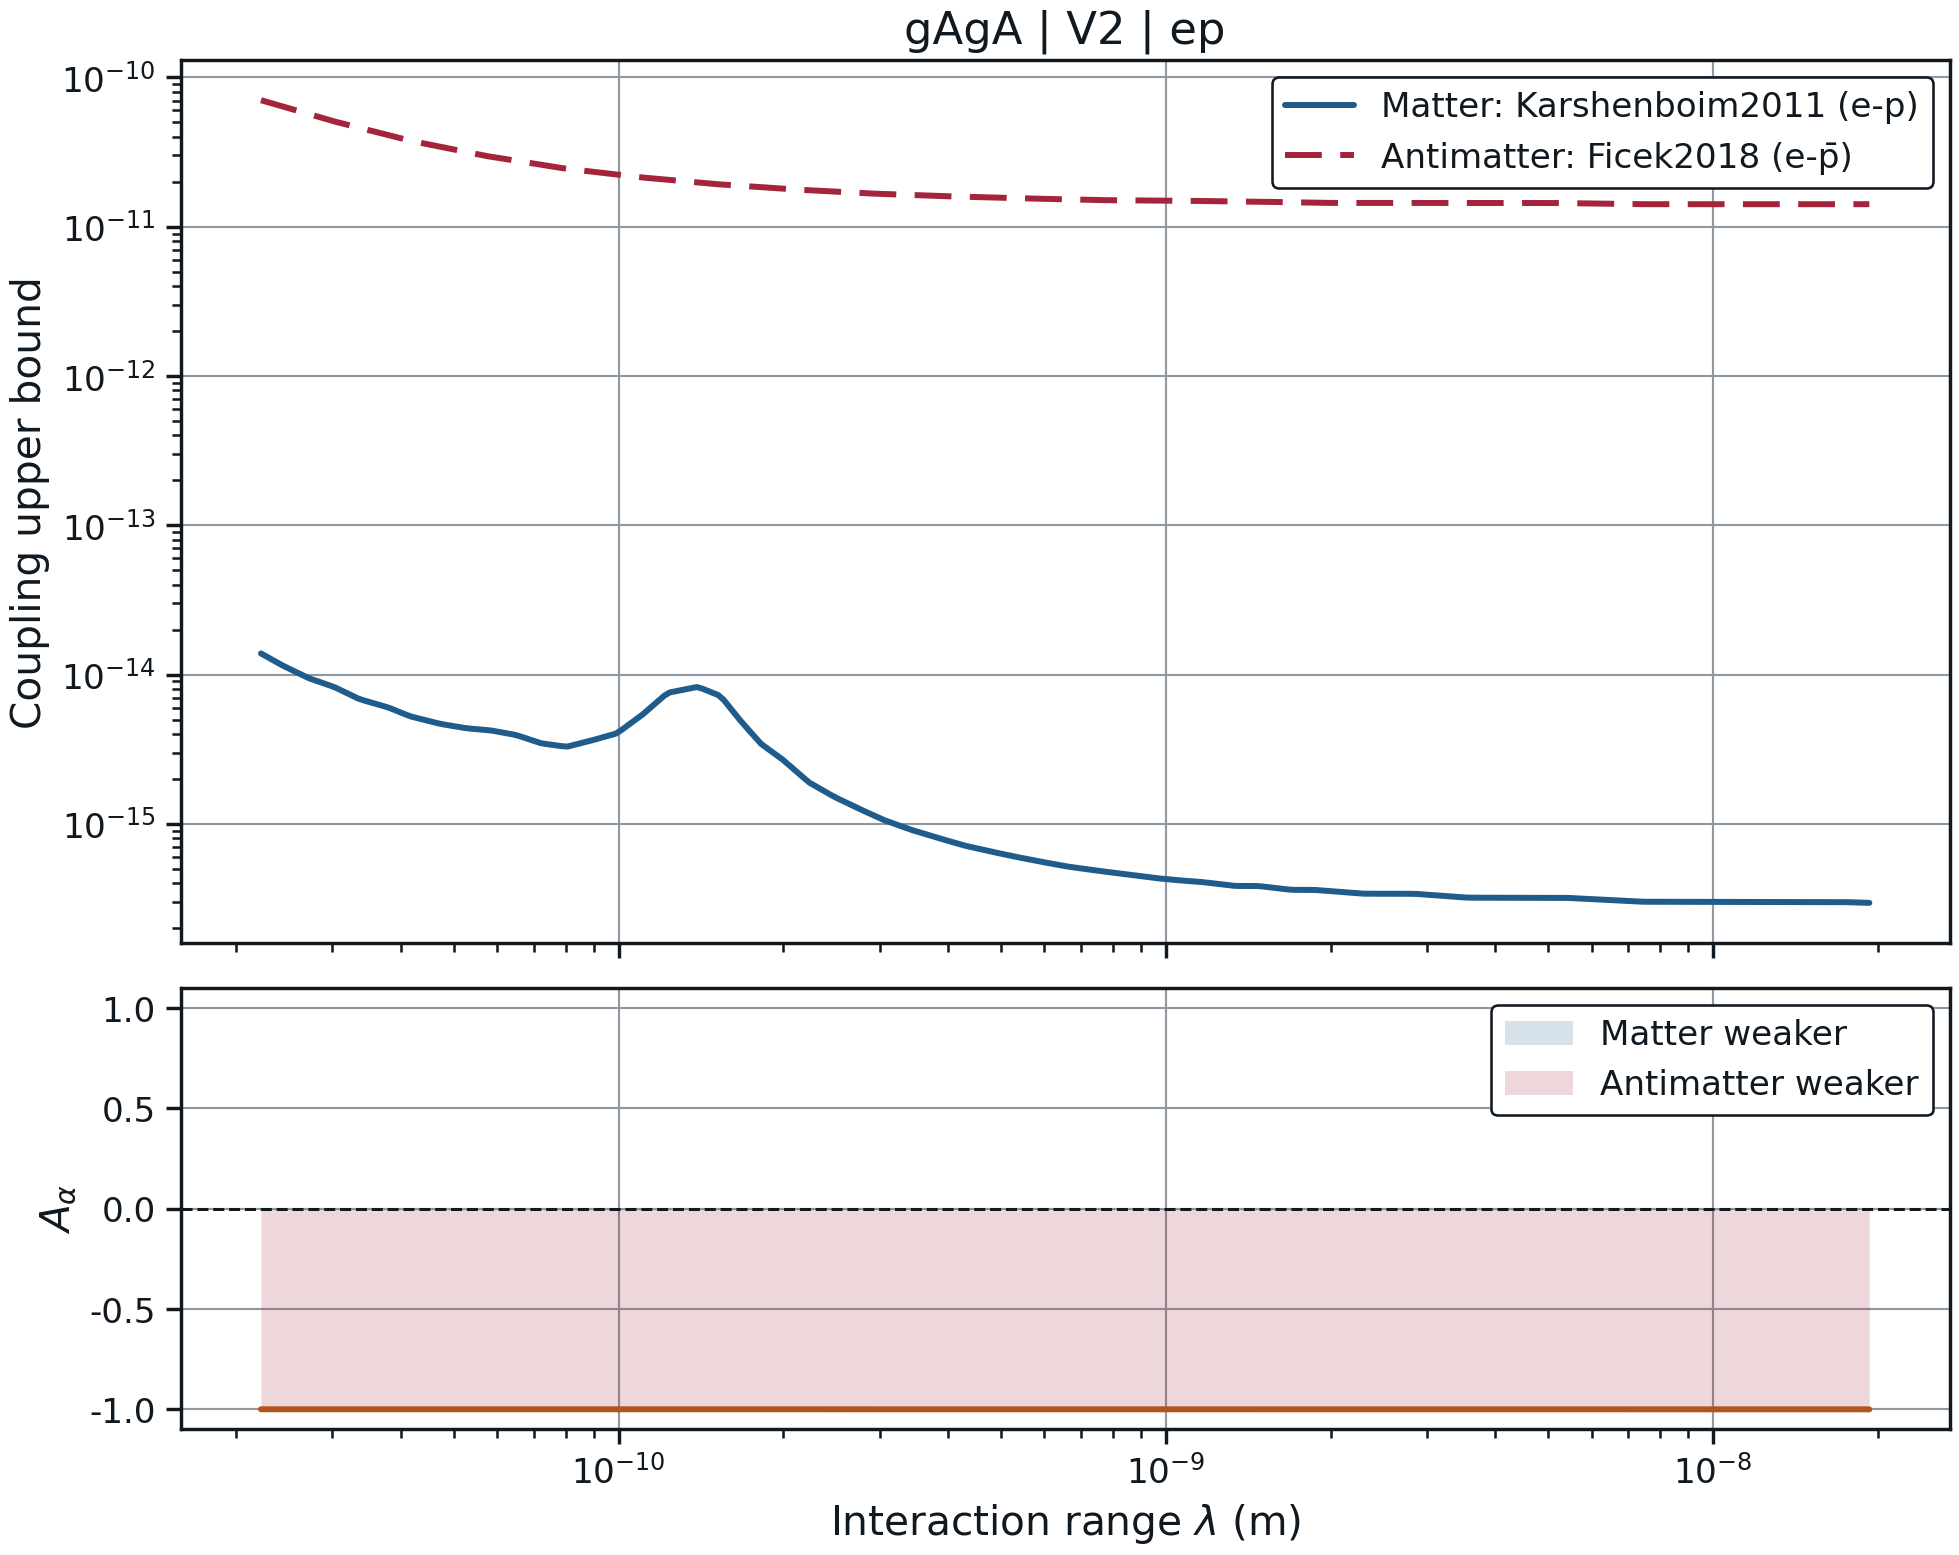
\includegraphics[width=0.75\textwidth]{gAgA_V2_ep_Karshenboim2011_vs_Ficek2018.png}
\caption{Matter--antimatter comparison for the $g_Ag_A\cdot V_2\cdot e$-$\bar p$ pair (Karshenboim, 2011, versus Ficek \textit{et al.}, 2018), one of the three highest asymmetries in the compiled database ($\overline{|A_\alpha|}=0.9998$).}
\label{fig:matter-antimatter}
\end{figure}
\clearpage

\begin{figure}[p]
\centering
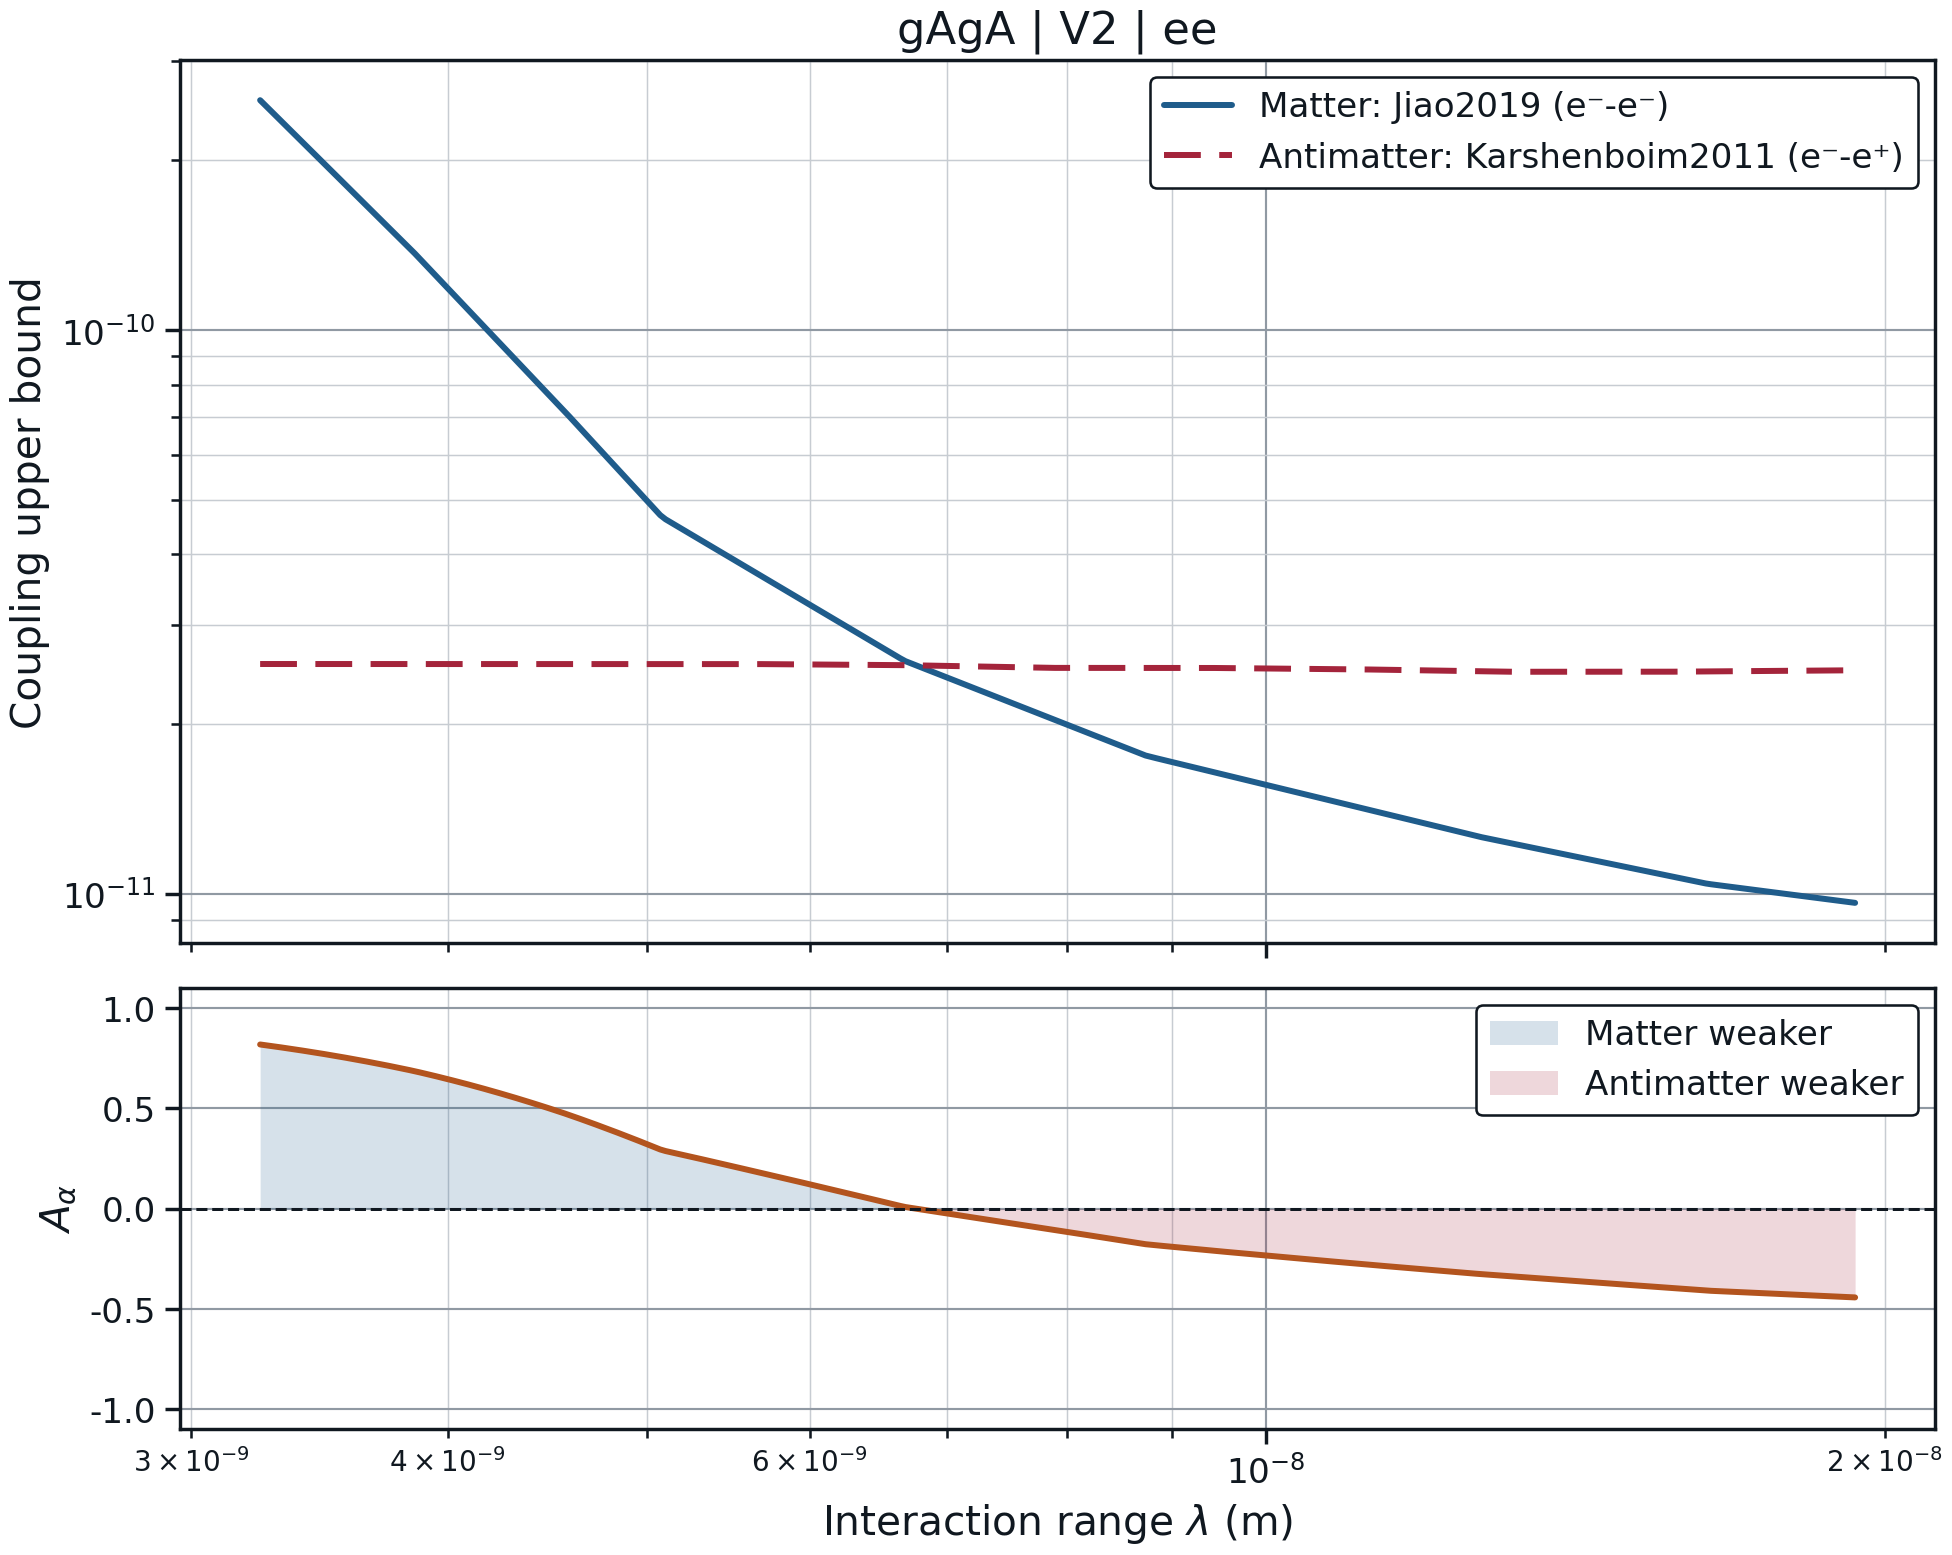
\includegraphics[width=0.75\textwidth]{gAgA_V2_ee_Jiao2019_vs_Karshenboim2011.png}
\caption{Matter--antimatter comparison for the $g_Ag_A\cdot V_2\cdot e$-$e^+$ pair (Jiao \textit{et al.}, versus Karshenboim, 2011), the lowest asymmetry in the compiled database ($\overline{|A_\alpha|}=0.334$), included alongside Figure~\ref{fig:matter-antimatter} to show that the analysis does not produce a saturated asymmetry for every pair by construction.}
\label{fig:matter-antimatter-lowest}
\end{figure}
\clearpage

\begin{figure}[p]
\centering
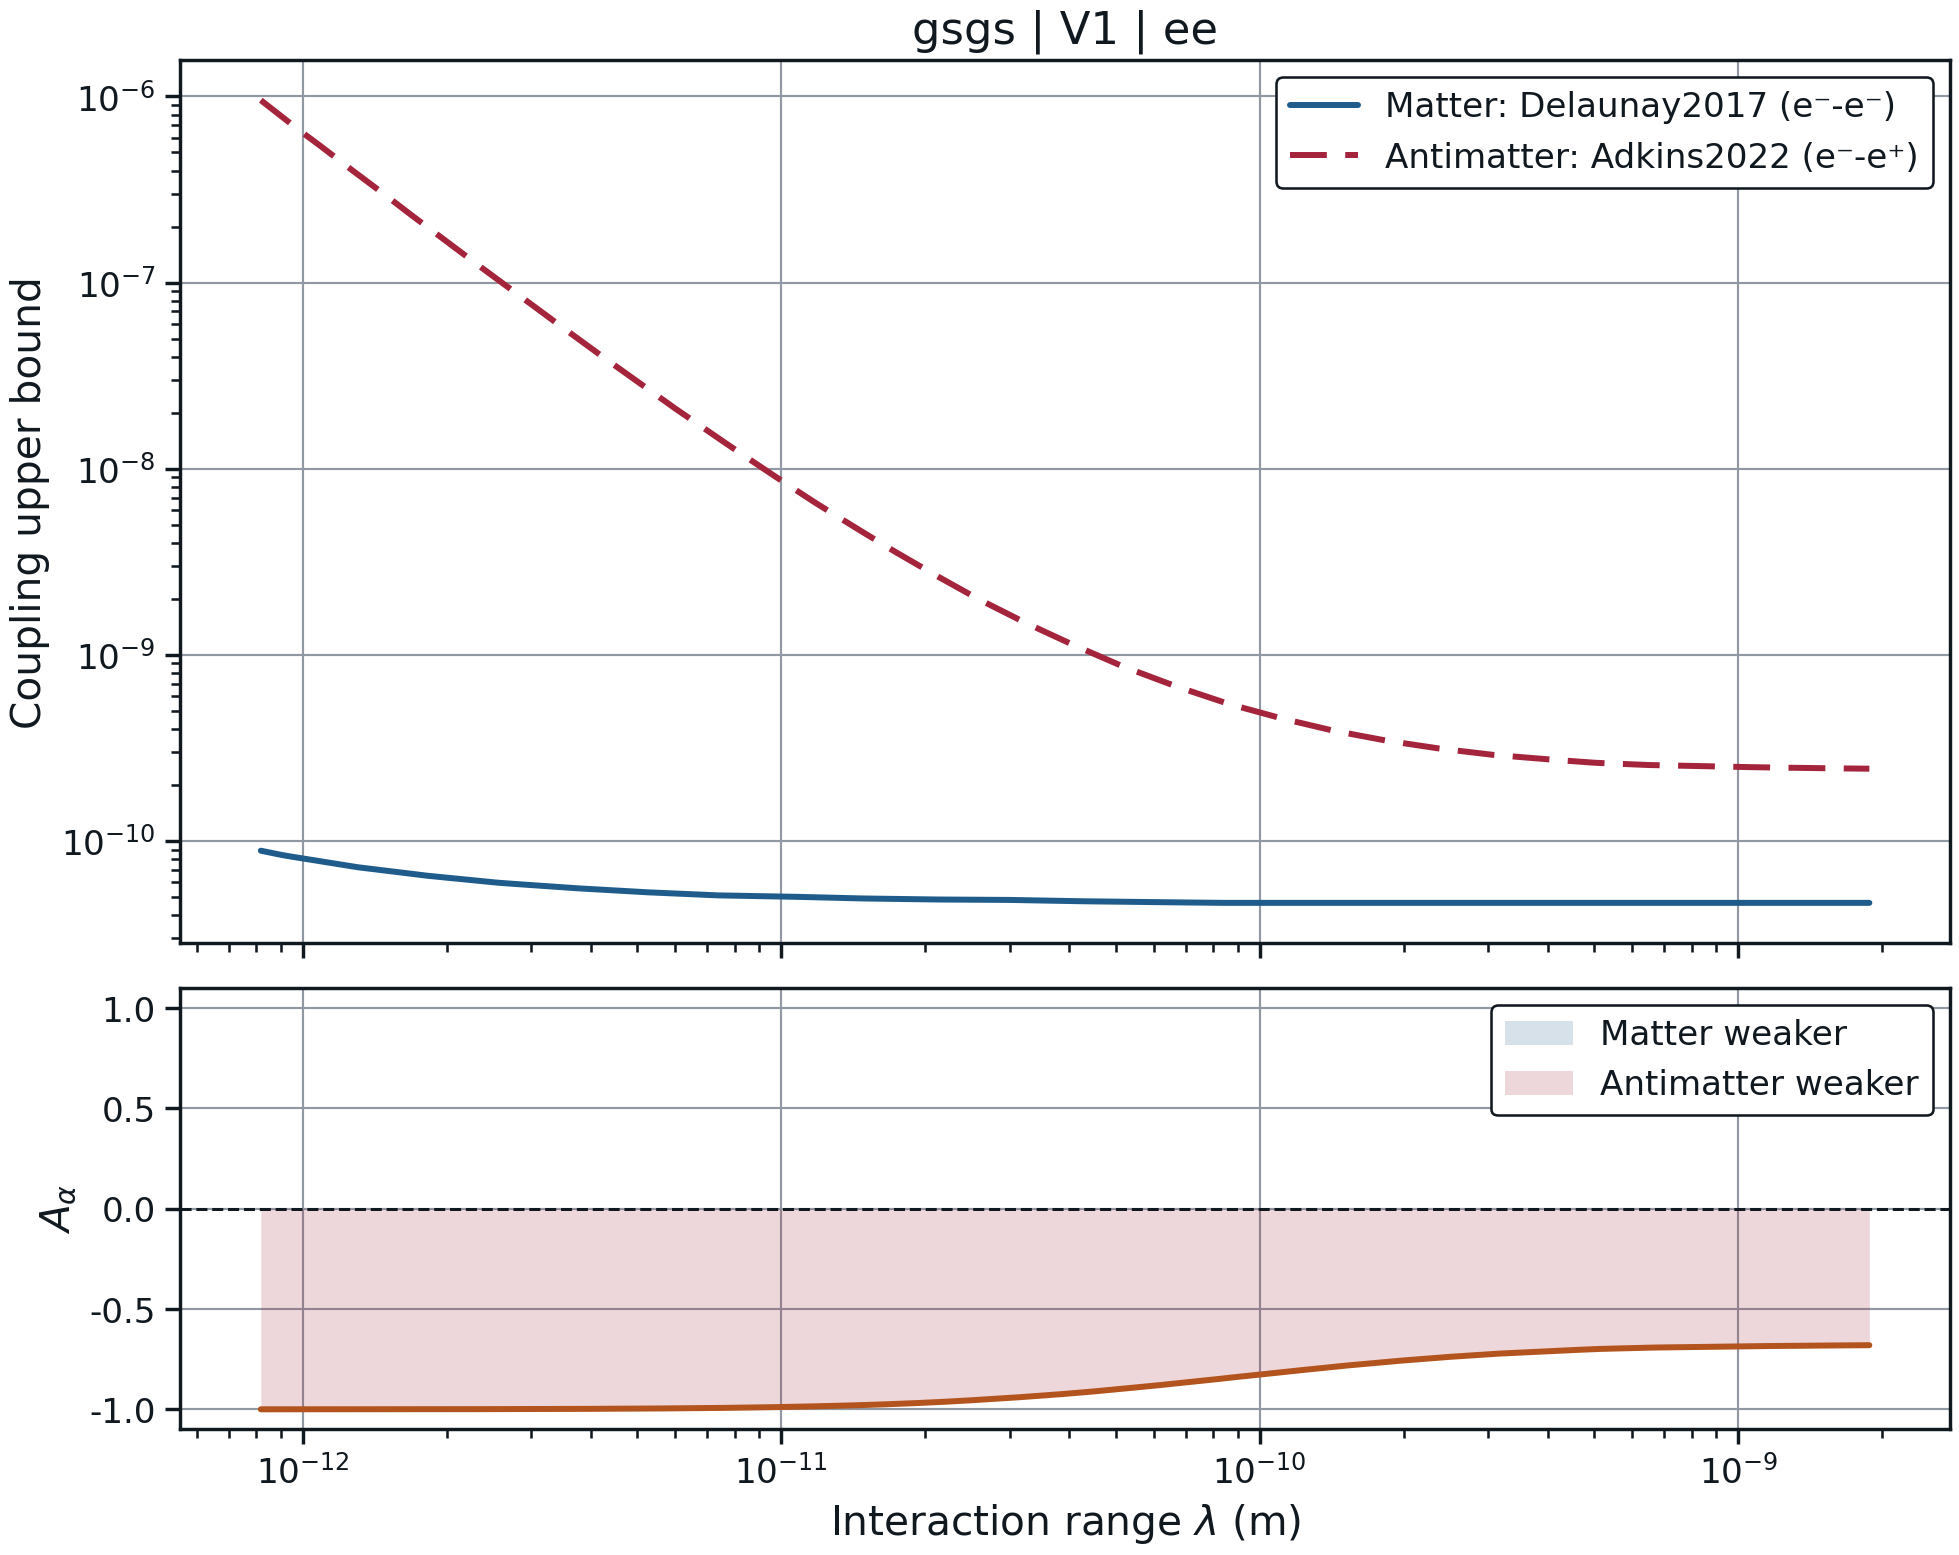
\includegraphics[width=0.75\textwidth]{gsgs_V1_ee_Delaunay2017_vs_Adkins2022.png}
\caption{Matter--antimatter comparison for the $g_sg_s\cdot V_1\cdot e$-$e^+$ pair (Delaunay \textit{et al.}, 2017, versus Adkins \textit{et al.}, 2022), the only currently matched $V_1$ pair. $V_1$ is spin-independent, so none of the four spin-dependent coefficients feeds it, yet its asymmetry is comparable to that of the spin-dependent pairs (see the discussion following Table~\ref{tab:pairs}).}
\label{fig:matter-antimatter-v1}
\end{figure}
\clearpage

\section{Gap Analysis}
\label{sec:results-gap}

\subsection{Coverage by Fermion Sector}

Table~\ref{tab:sector-gaps} compares the number of analysed datasets on
each side of the eleven canonical matter--antimatter \emph{sector} pairs
used by SPINDEP. These are pairings of fermion sectors, not the matched
dataset pairs of Section~\ref{sec:results-asym}.

\begin{table}[h]
\centering
\begin{tabular}{@{}l l r r >{\raggedright\arraybackslash}p{3.2cm}@{}}
\toprule
Matter sector & Antimatter sector & Matter & Antimatter & Status \\
\midrule
$e$-$e$     & $e$-$e^+$      & 40 & 5 & Populated (used above) \\
$e$-$p$     & $e$-$\bar p$   & 17 & 9 & Populated (used above) \\
$e$-$\mu$   & $e$-$\bar\mu$  & 0  & 6 & Antimatter only (muonium) \\
$e$-$n$     & $e$-$\bar n$   & 16 & 0 & \textbf{Gap} \\
$\mu$-$\mu$ & $\mu$-$\bar\mu$& 1  & 0 & \textbf{Gap} (thin on both sides) \\
$n$-$p$     & $n$-$\bar p$   & 9  & 0 & \textbf{Gap} \\
$n$-$n$     & $n$-$\bar n$   & 8  & 0 & \textbf{Gap} \\
$p$-$p$     & $p$-$\bar p$   & 0  & 0 & No data either side \\
$e$-$N$     & $e$-$\bar N$   & 50 & 0 & \textbf{Largest gap} \\
$n$-$N$     & $n$-$\bar N$   & 49 & 0 & \textbf{Gap} (second largest) \\
$p$-$N$     & $p$-$\bar N$   & 18 & 0$^\dagger$ & \textbf{Gap} in comparable units \\
\bottomrule
\end{tabular}
\caption{Matter versus antimatter dataset counts per canonical fermion
sector pair. $^\dagger$A $\bar p$-$N$ bound does exist, from the antiprotonic-helium
spectroscopy analysed by Salumbides \textit{et al.} (2014); it is excluded from this count
because it is published as a gravity-normalised strength $|\alpha|$ rather
than a coupling bound $|g|$ and so cannot be compared with the $p$-$N$
datasets without a conversion this framework does not perform. The gap in
\emph{comparable} data is therefore real, but it is a unit-conversion gap
rather than an absence of measurement.}
\label{tab:sector-gaps}
\end{table}

The three nucleus sectors dominate the gap. $e$-$N$ is the single largest
opportunity in the database, with 50 matter-sector datasets against zero in
$e$-$\bar N$, but $n$-$N$ is barely behind it at 49, and $p$-$N$ adds a
further 18; between them these three account for 117 of the 225
matter-sector datasets and carry no antimatter-sector counterpart at all.
The $e$-$n$, $n$-$p$, and $n$-$n$ sectors each have a smaller but still
substantial matter-sector base (8--16 datasets), again with no
antimatter-sector counterpart. The $e$-$\mu$ row is the mirror image: all
six of its bounds come from muonium and so sit on the antimatter side, with
no matter-sector $e$-$\mu$ bound to compare them with.

The eleven sector pairs in Table~\ref{tab:sector-gaps} account for 208
matter-sector and 20 antimatter-sector datasets, 228 in all, of the 247
analysed. (The two antimatter datasets not shown are the $\bar p$-He and
$dd\mu^+$ entries, whose sectors have no counterpart row; this is why the
table's antimatter column totals 20 rather than the 22 quoted in
Section~\ref{sec:results-db}.) The remaining 19 do not belong to a matter--antimatter
sector pair at all: 16 are astrophysical bounds, quoted for a single sector
with no laboratory antimatter counterpart, and the other three are the
$\mu$-$N$, $\bar p$-He and $dd\mu^+$ entries, whose sectors have no
counterpart row in the table.

\subsection{Coverage by Dobrescu--Mocioiu Potential}

Table~\ref{tab:potential-gaps} breaks the same comparison down by DM
potential.

\begin{table}[h]
\centering
\begin{tabular}{@{}l r r >{\raggedright\arraybackslash}p{4.5cm}@{}}
\toprule
Potential & Matter datasets & Antimatter datasets & Status \\
\midrule
$V_{4+5}$  & 58 & 3 & Thin antimatter coverage \\
$V_{9+10}$ & 31 & 0 & \textbf{Gap} \\
$V_3$      & 29 & 10 & Best-covered potential (used throughout Section~\ref{sec:results-asym}) \\
$V_{1a}$   & 14 & 0 & \textbf{Gap} \\
$V_2$      & 17 & 3 & Thin antimatter coverage \\
$V_1$      & 42 & 5 & Thin antimatter coverage \\
$V_{12+13}$& 16 & 0 & \textbf{Gap} \\
$V_{11}$   & 7  & 0 & \textbf{Gap} \\
$V_8$      & 5  & 1 & Thin antimatter coverage \\
$V_{15}$   & 2  & 0 & \textbf{Gap} \\
$V_{16}$   & 2  & 0 & \textbf{Gap} \\
$V_{2+3}$  & 2  & 0 & \textbf{Gap} (combination label) \\
\bottomrule
\end{tabular}
\caption{Matter versus antimatter dataset counts per Dobrescu--Mocioiu potential.}
\label{tab:potential-gaps}
\end{table}

Seven of the twelve classified potentials, $V_{11}$, $V_{15}$, $V_{16}$,
$V_{1a}$, $V_{9+10}$, $V_{12+13}$, and $V_{2+3}$, have \emph{zero}
antimatter-sector datasets. Only $V_3$ has antimatter coverage exceeding a
handful of datasets, which is why fourteen of the fifteen matched pairs in
Section~\ref{sec:results-asym} involve $V_2$ or $V_3$.

Figures~\ref{fig:lambda-coverage-v1}--\ref{fig:matter-antimatter-ratio} show
the dataset inventory and coverage matrix for the same database. They count
\emph{independent bounds} rather than dataset files: 48 of the 247 analysed
datasets are the same measured bound filed under more than one coupling
family, and are collapsed to a single curve before plotting, leaving 199
independent bounds. Row and column totals read off those figures are
therefore systematically smaller than the counts in Tables
\ref{tab:sector-gaps} and~\ref{tab:potential-gaps}, which count files as the
registry records them. The two views agree on every gap; they differ only
in how multiply-filed bounds are counted.

\clearpage
\begin{figure}[p]
\centering
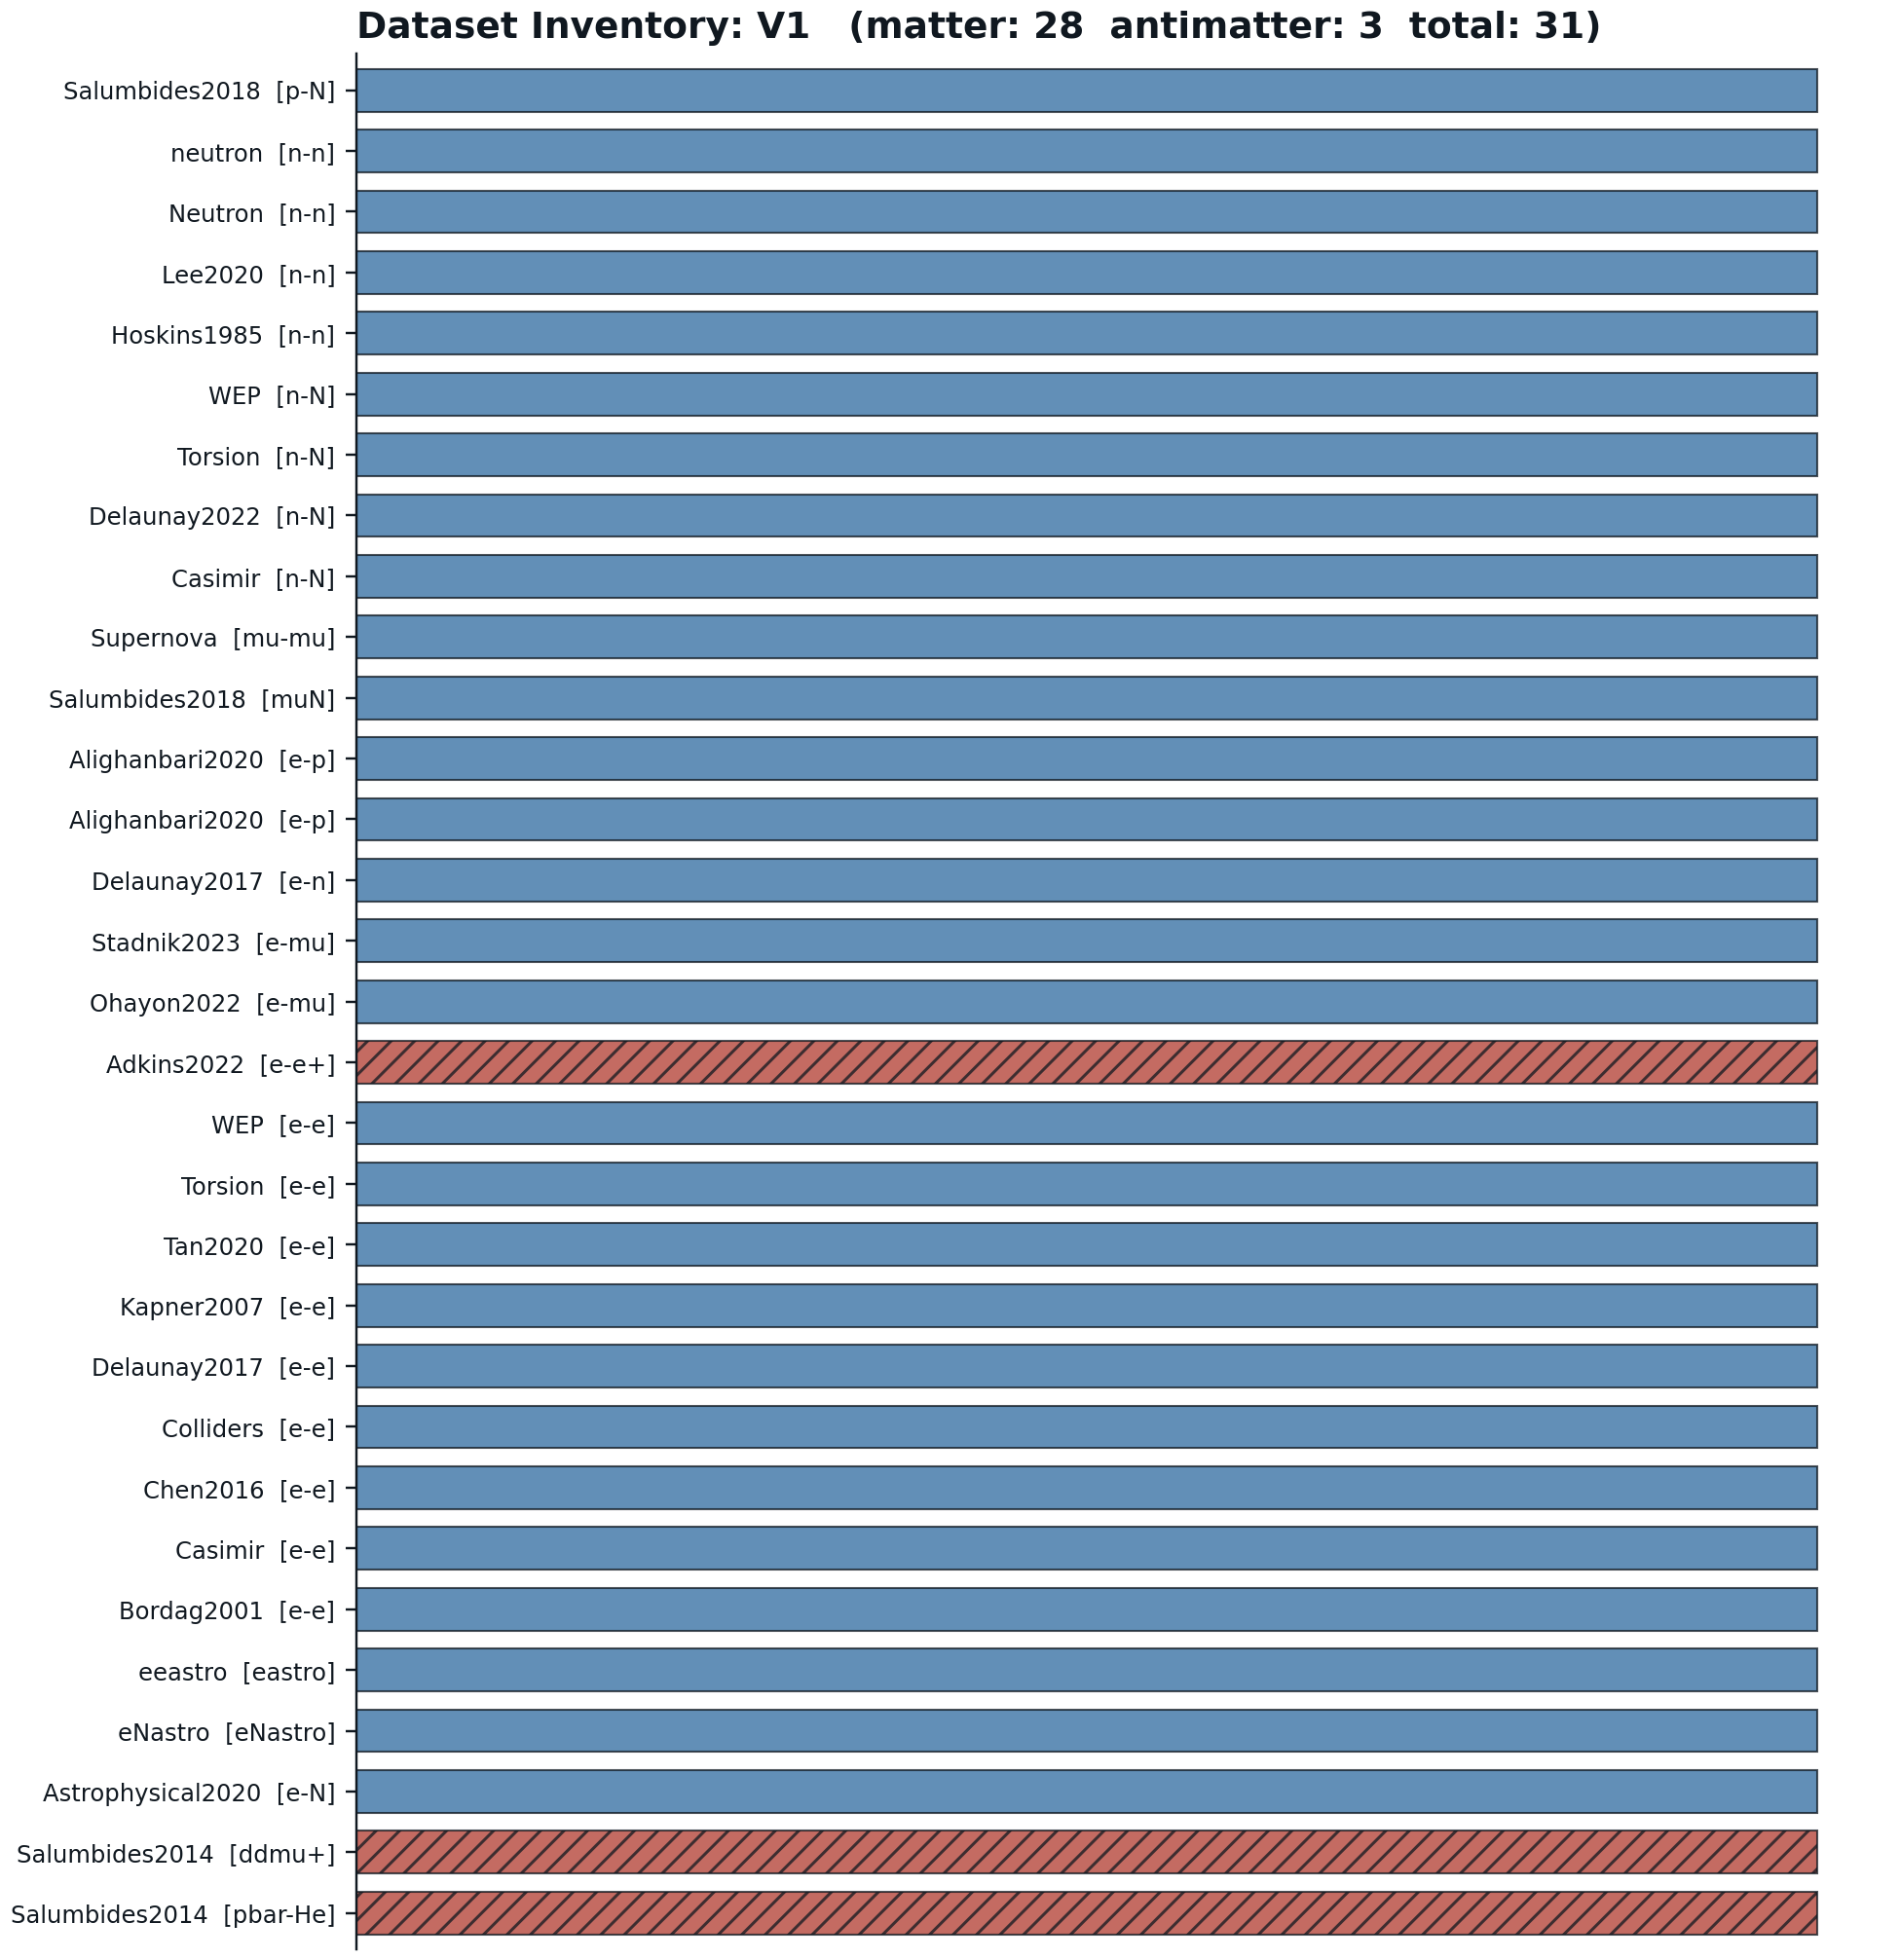
\includegraphics[width=0.85\textwidth,height=0.9\textheight,keepaspectratio]{lambda_coverage_V1.png}
\caption{Dataset inventory for $V_1$.}
\label{fig:lambda-coverage-v1}
\end{figure}
\clearpage

\begin{figure}[p]
\centering
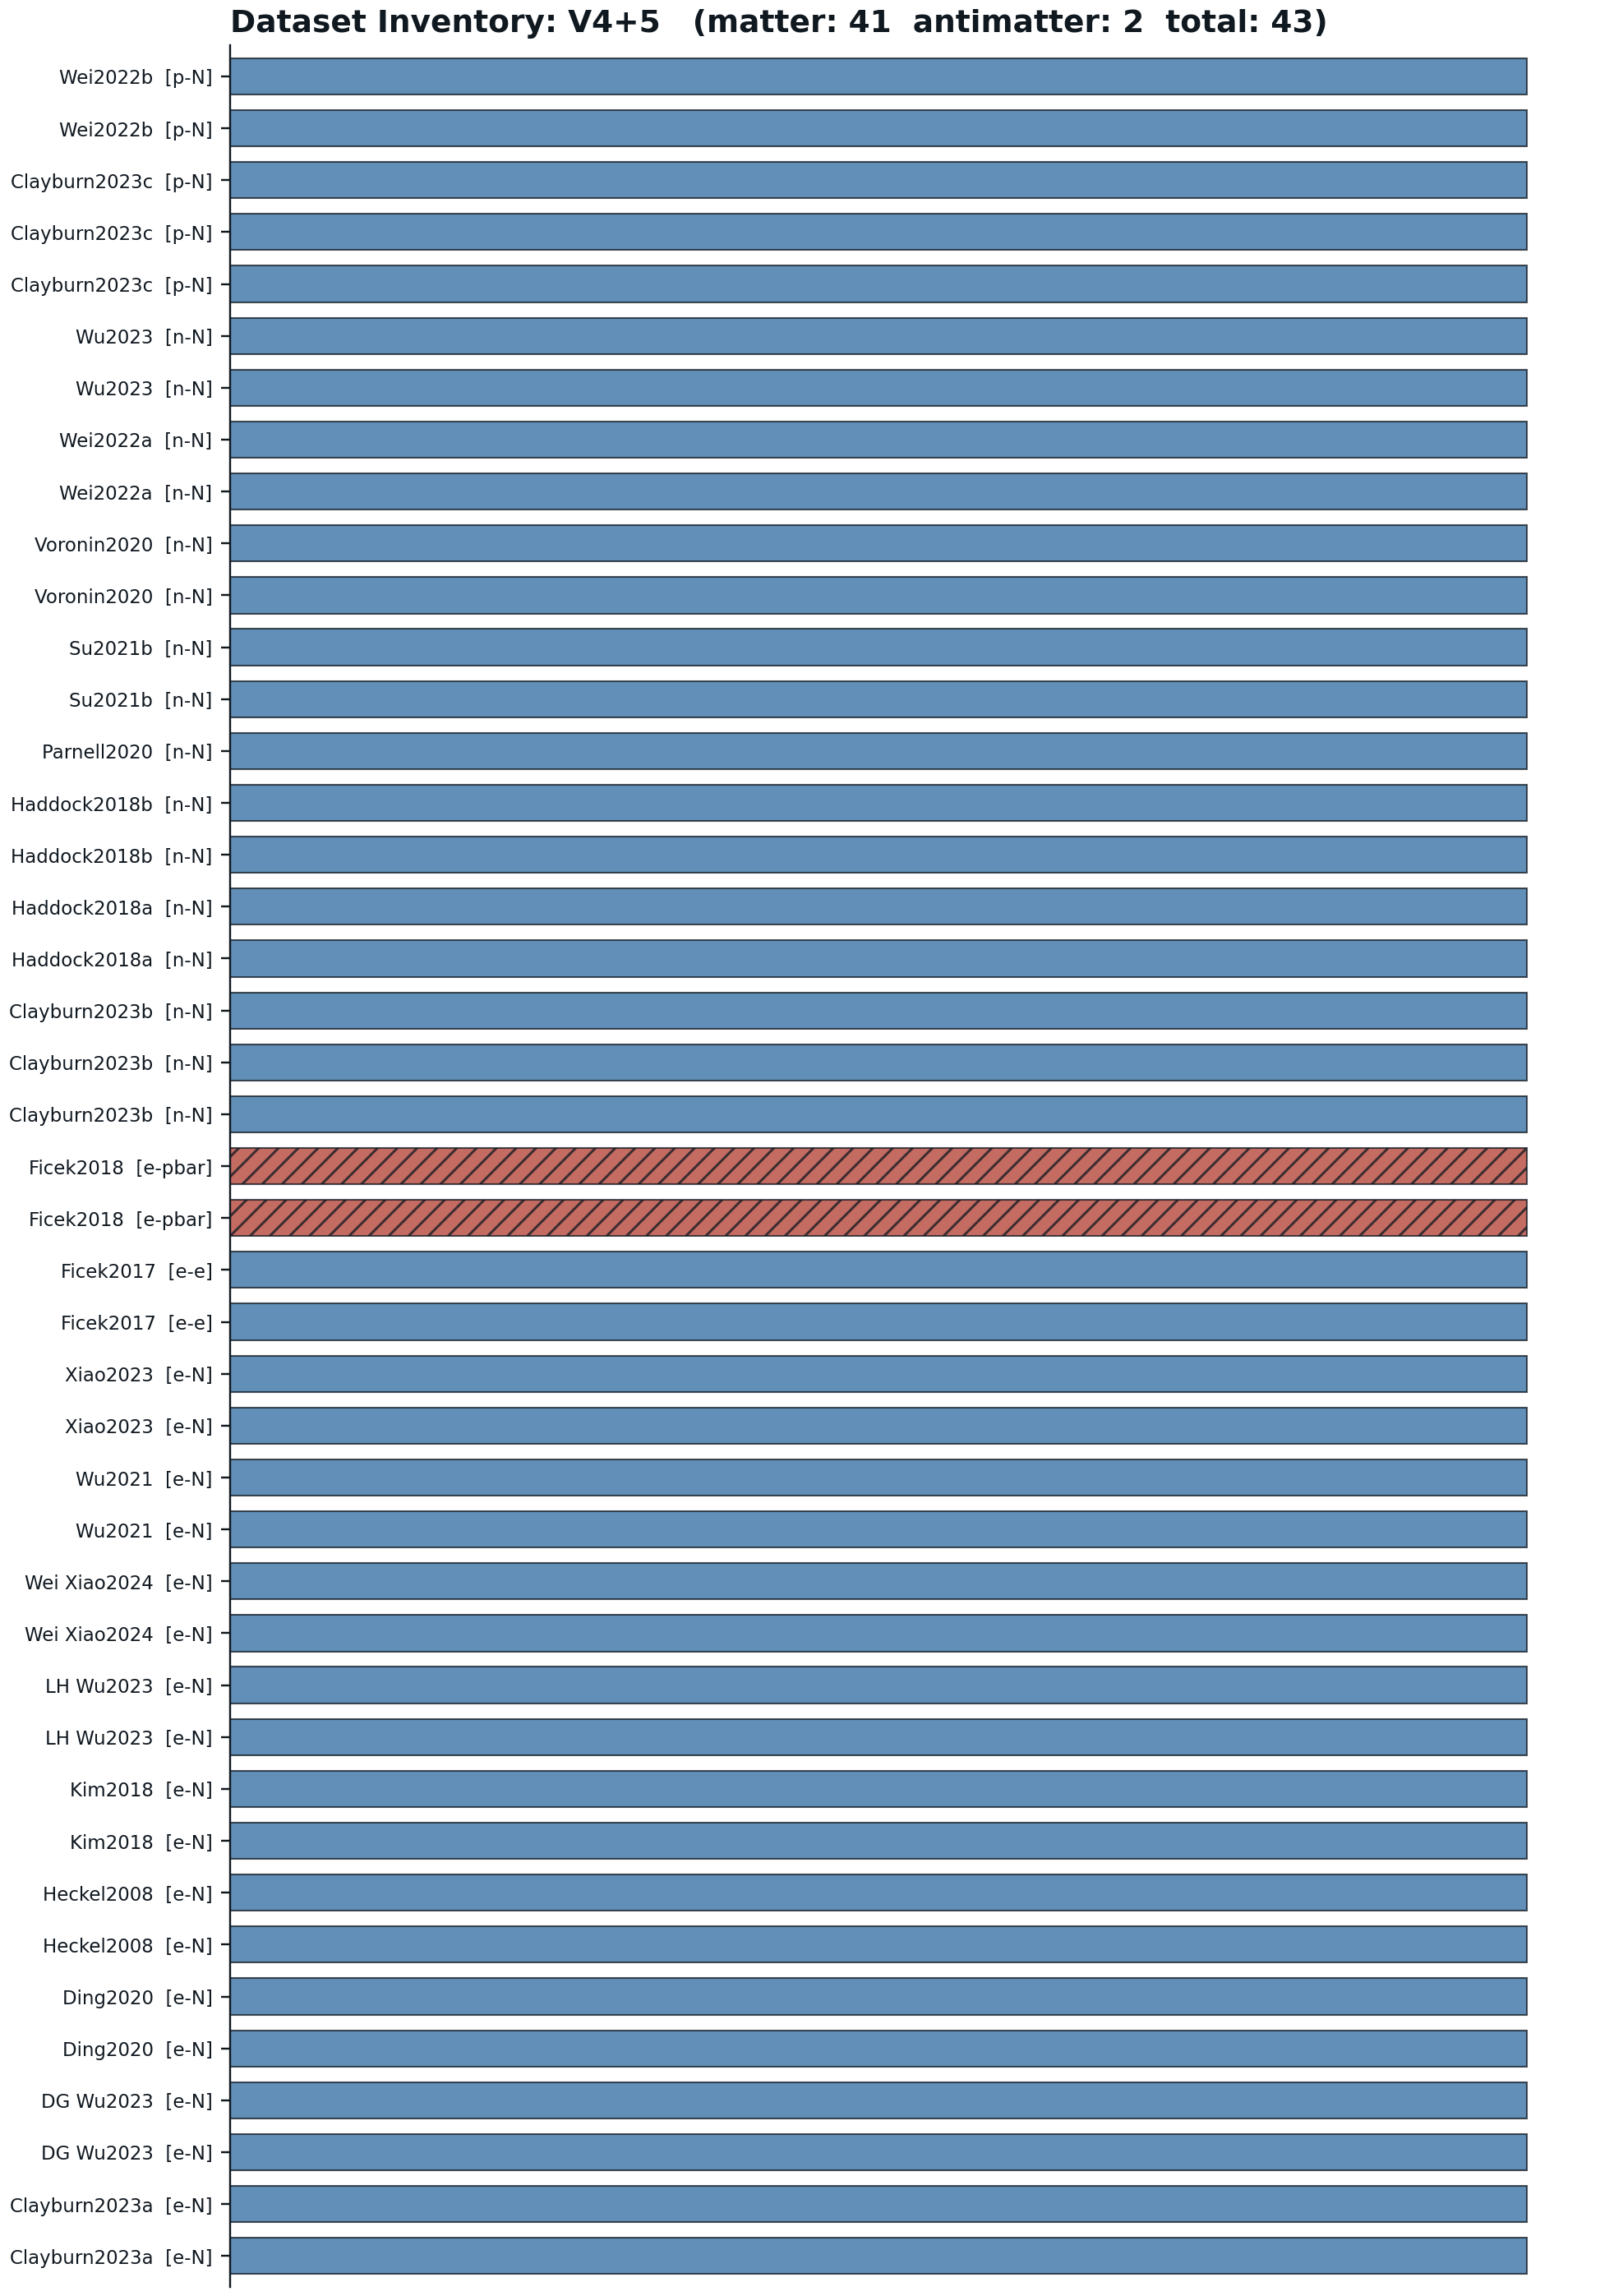
\includegraphics[width=0.85\textwidth,height=0.9\textheight,keepaspectratio]{lambda_coverage_V4p5.png}
\caption{Dataset inventory for $V_{4+5}$, the most populated potential in the database (61 datasets).}
\label{fig:lambda-coverage-v45}
\end{figure}
\clearpage

\begin{figure}[p]
\centering
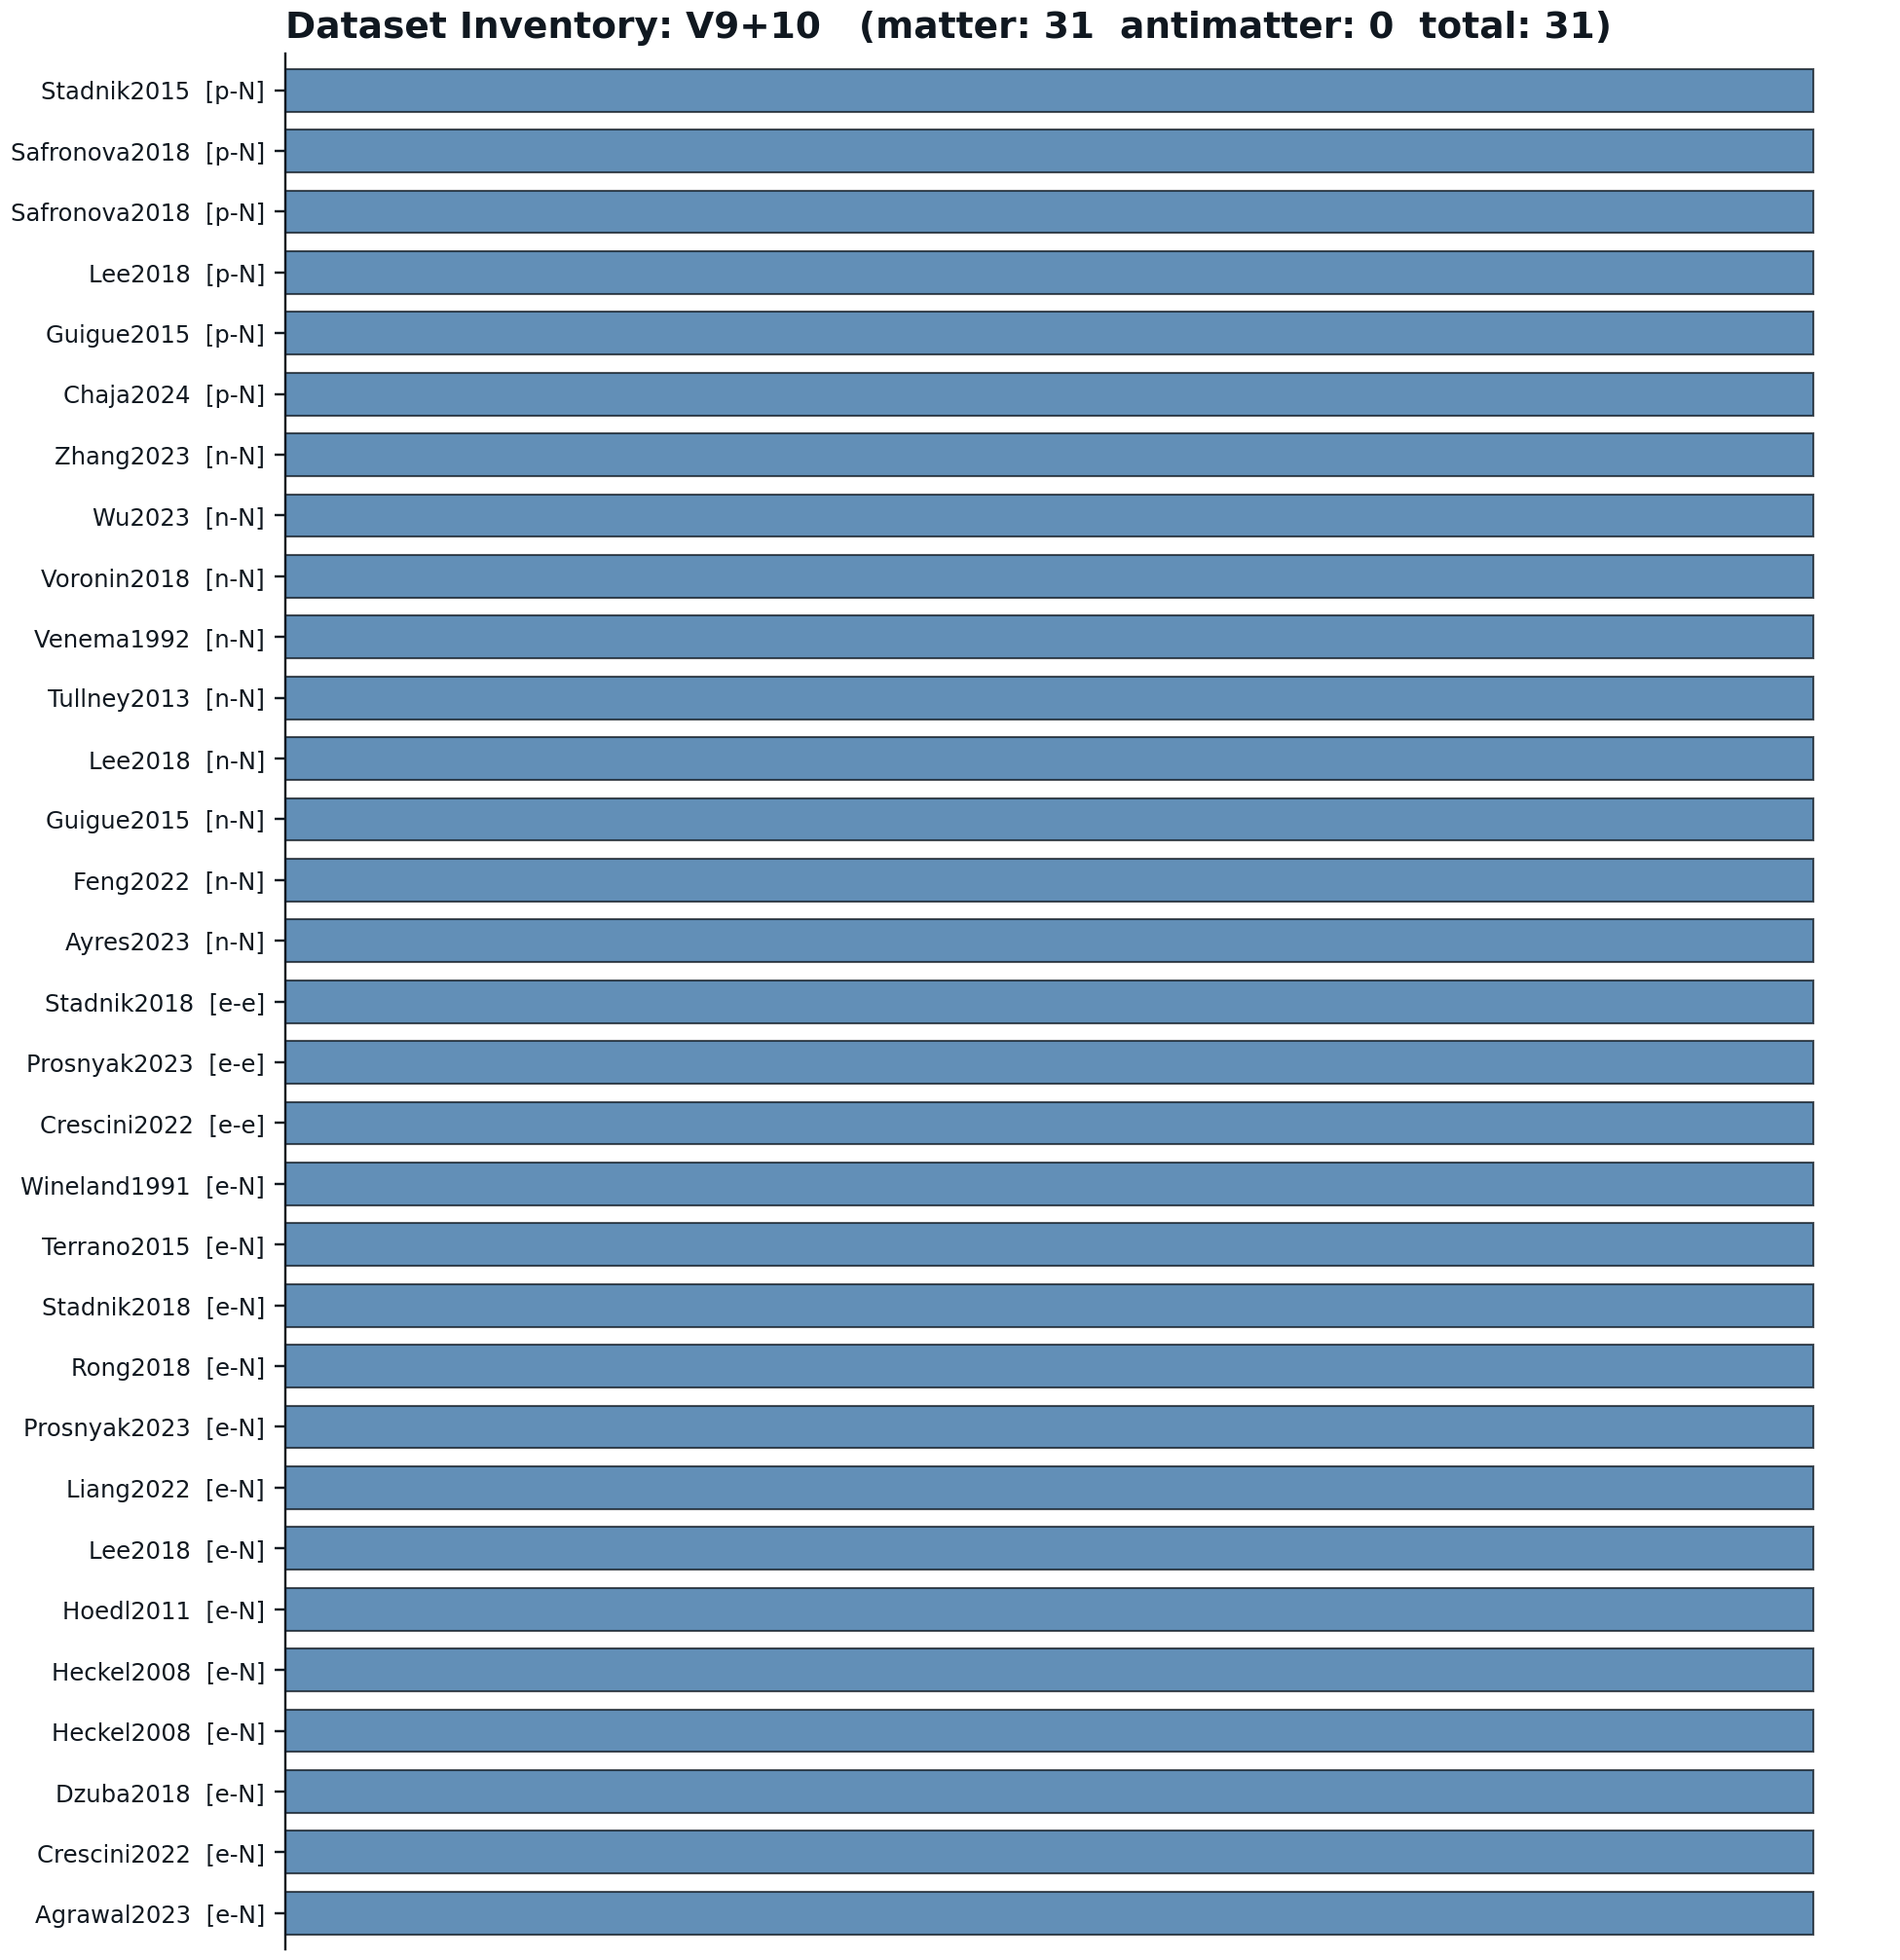
\includegraphics[width=0.85\textwidth,height=0.9\textheight,keepaspectratio]{lambda_coverage_V9p10.png}
\caption{Dataset inventory for $V_{9+10}$.}
\label{fig:lambda-coverage-v910}
\end{figure}
\clearpage

\begin{figure}[p]
\centering
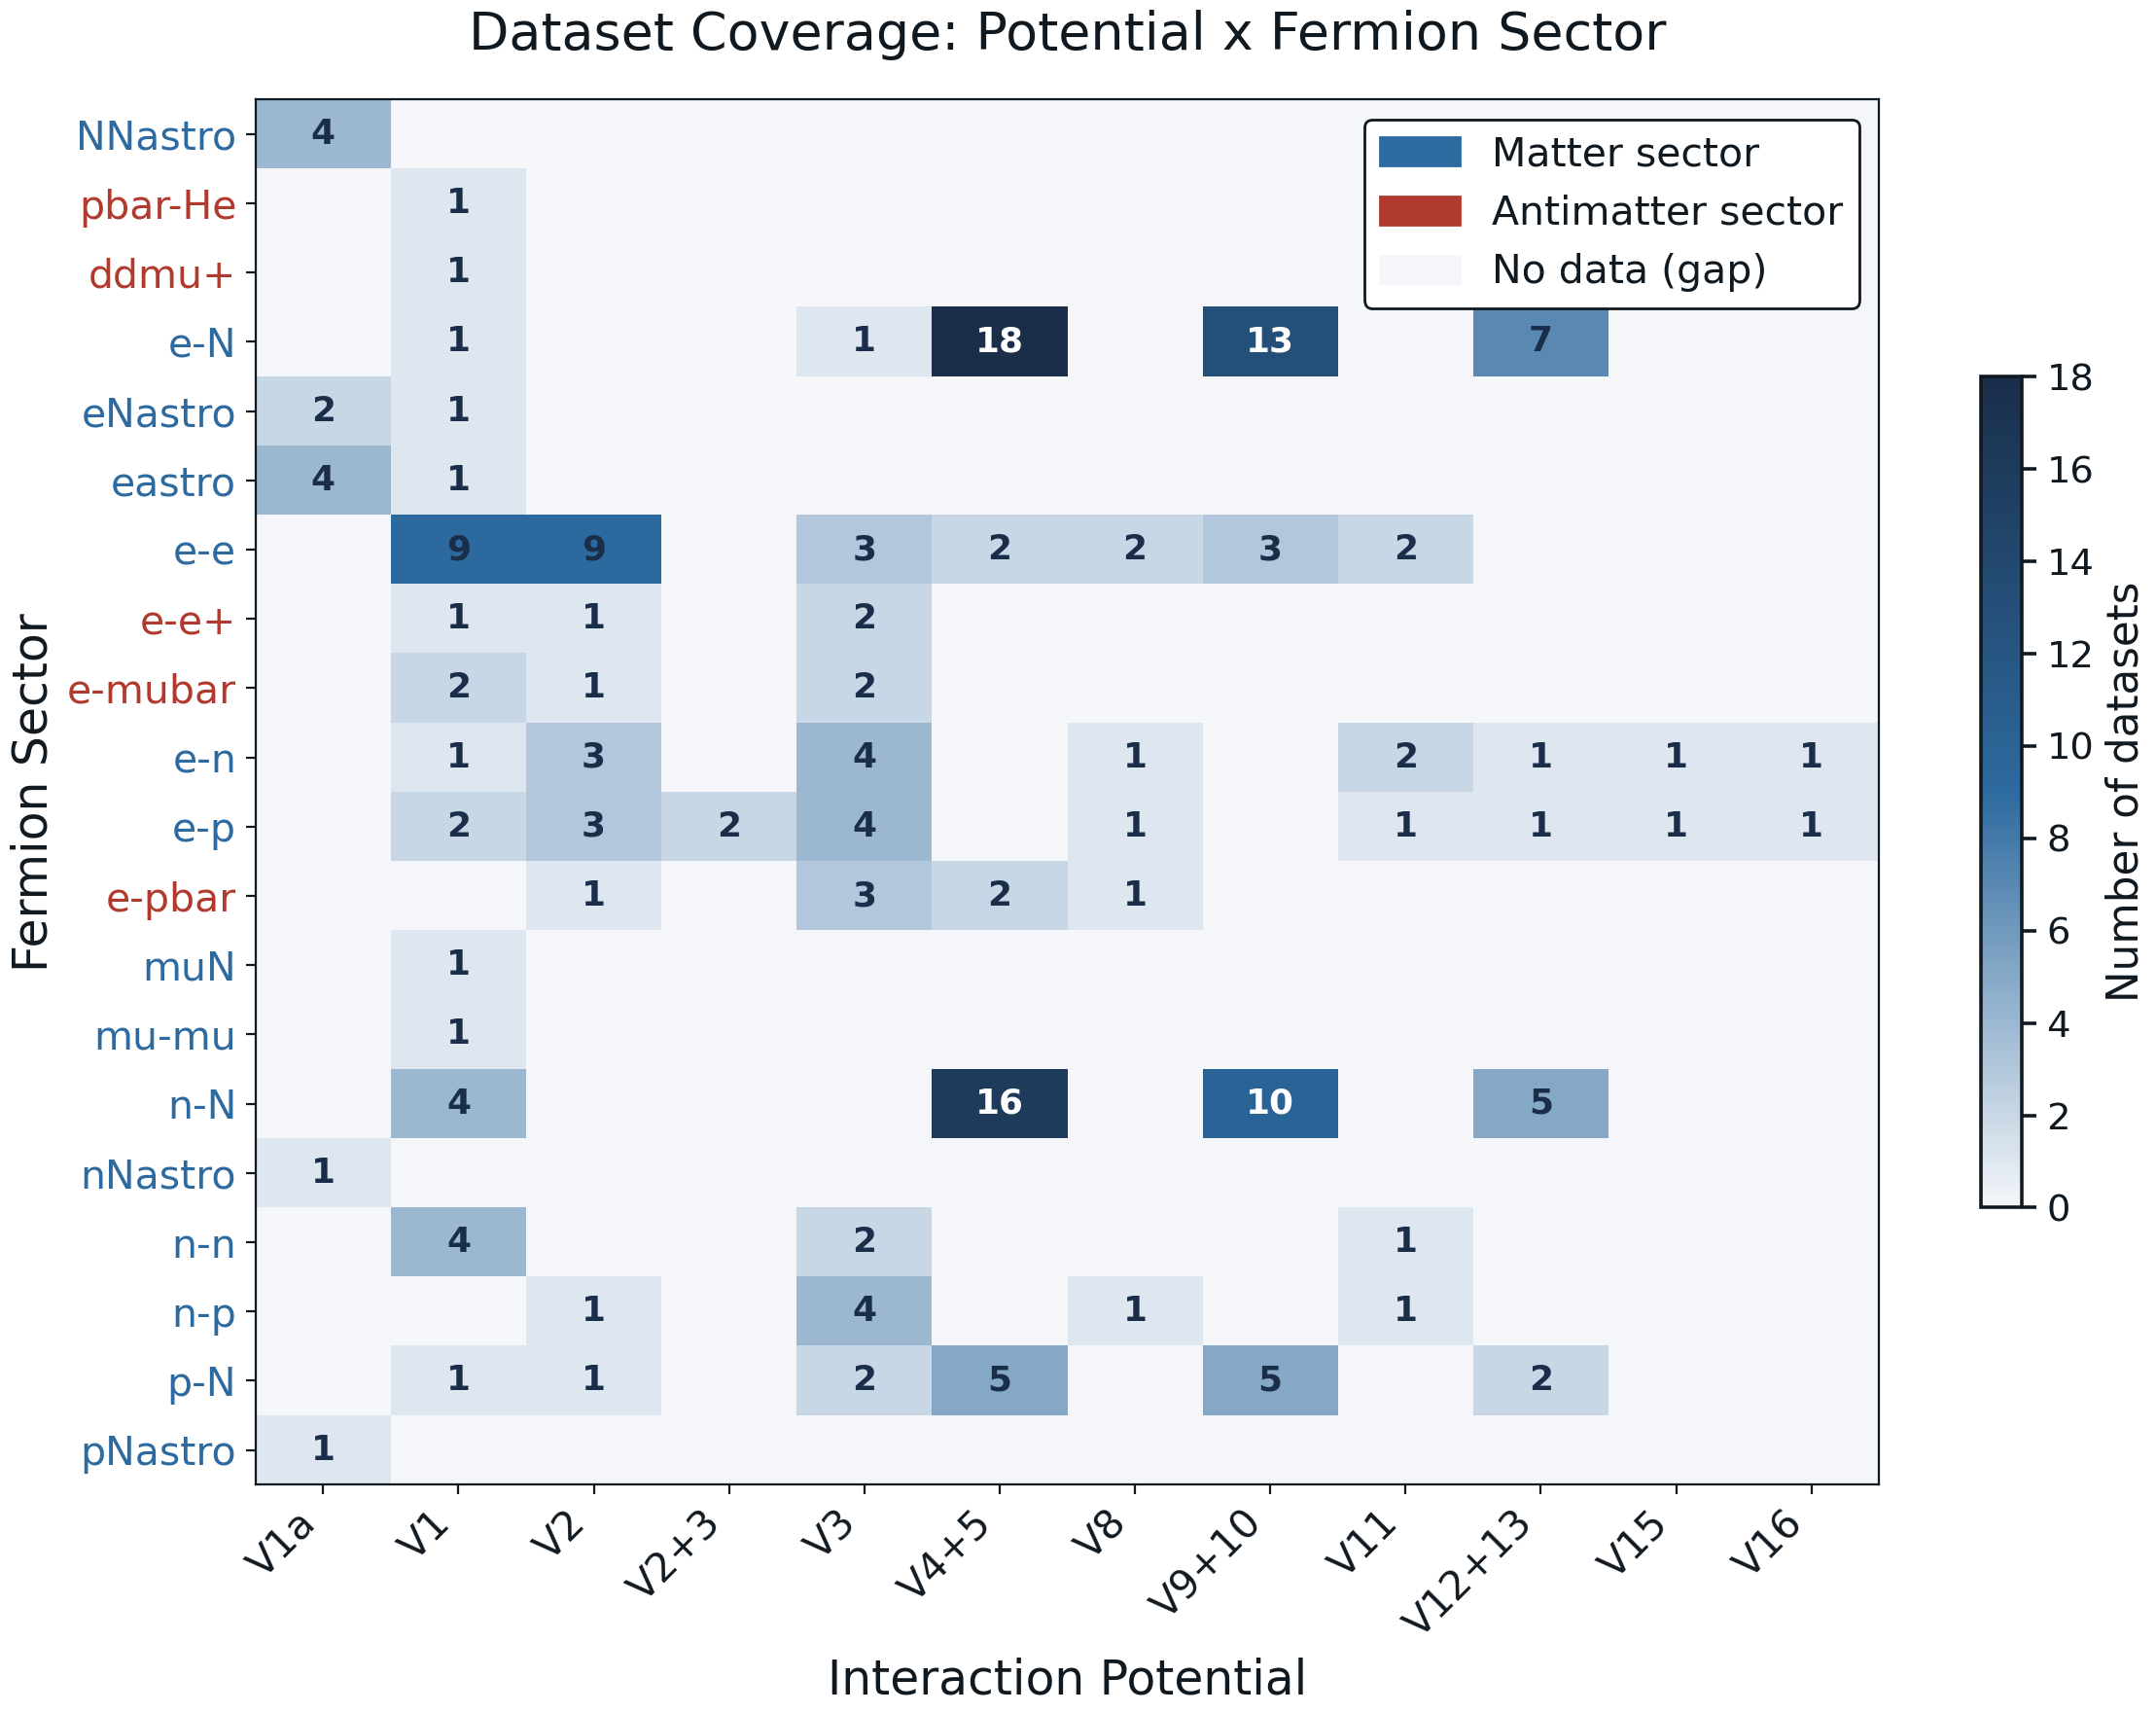
\includegraphics[width=0.75\textwidth]{pair_coverage_matrix.png}
\caption{Dataset count by potential and sector; antimatter-sector rows are
highlighted. Cells count independent bounds, not dataset files, so totals
fall below those in Tables~\ref{tab:sector-gaps}
and~\ref{tab:potential-gaps}; the gaps identified are the same.}
\label{fig:pair-coverage}
\end{figure}
\clearpage

\begin{figure}[p]
\centering
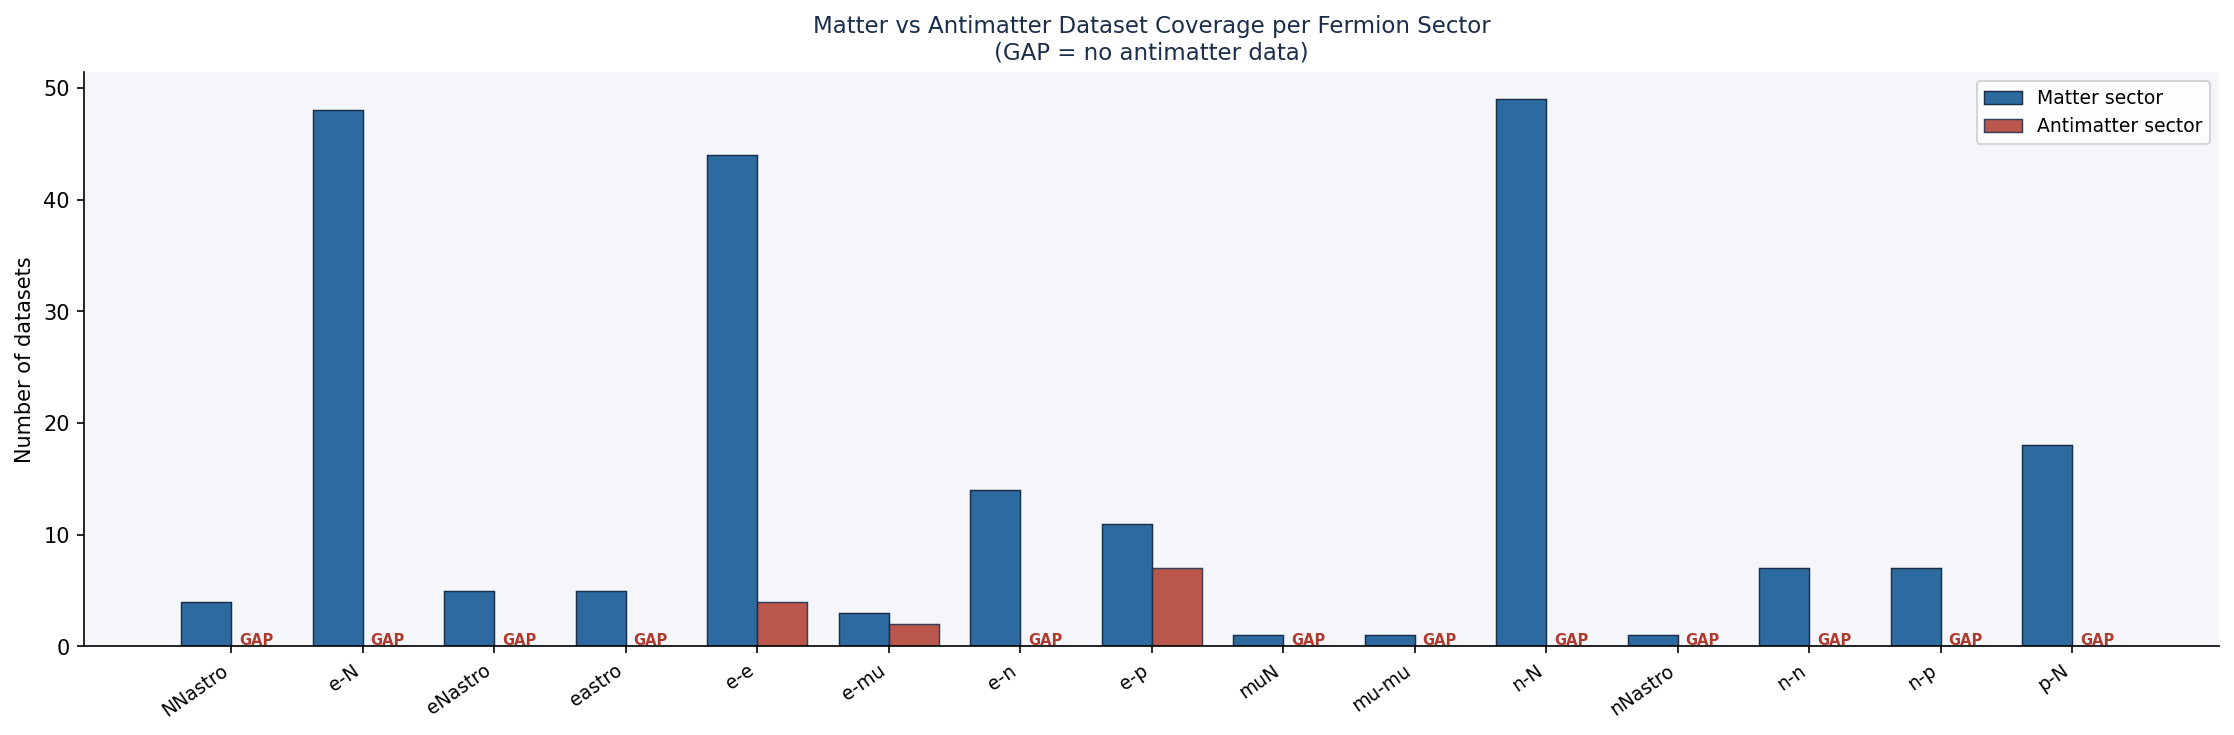
\includegraphics[width=0.75\textwidth]{matter_antimatter_ratio.png}
\caption{Matter-to-antimatter dataset count ratio by sector and potential.}
\label{fig:matter-antimatter-ratio}
\end{figure}
\clearpage

\subsection{Data-Quality and Framework Limitations}

Two limitations of the current database and framework are distinct from
the physics coverage gaps above and are stated here rather than worked
around silently. First, the 36 datasets held out of the analysis
(Section~\ref{sec:results-db}) are excluded rather than reclassified, and
the reasons differ in kind. Twenty-eight are \texttt{Combined} envelope
curves, twelve in $g_Ag_V$ and sixteen in $g_pg_s$, which the source
database marks \texttt{review\_only} and assigns no potential; these are
not a parsing gap that any filename convention could close, because no
single $V_n$ describes an envelope over several experiments, and they
would have to be decomposed into their constituent bounds before they
could enter a per-potential analysis. The sixteen $g_pg_s$ curves were
identified only when every potential assignment in the database was
validated against the source database's curation records: a local
filename prefix had caused them to be read as $V_{1a}$, which those
records contradict. Two are
contributor-template placeholders, and were previously being read as $V_1$
and $V_2$ datasets on the strength of a trailing digit in their filenames,
which inflated those two potentials by one dataset each. The remaining one
is a $g_pg_p$ astrophysical $e$-$N$ bound: a real measurement, but one whose
potential is unassigned upstream, and assigning it $V_{1a}$ from the
filenames of its siblings in other coupling families would be an inference
rather than evidence. It is held out until the source publication settles
it, and is the one exclusion that a single documentary check could reverse.
The last five are the 90\% CL Cong \textit{et al.} (2025) curves, excluded
as duplicates of the 95\% CL set rather than as defective data; retaining
both would count one experiment twice.
Second, six entries under $V_3$, $V_{9+10}$ and $V_{15}$ report
interaction ranges that are physically implausible, reaching
$\lambda\sim10^{52}$~m against an observable universe of order
$10^{26}$~m, almost certainly the result of a unit token being mis-detected
during compilation. Three of the fifteen matched pairs in
Table~\ref{tab:pairs} draw on an affected dataset: the $g_Ag_A\cdot
V_3\cdot e$-$e^+$ pair on the matter side (Ficek \textit{et al.}, 2017),
and the two $g_Ag_A\cdot V_3\cdot e$-$\bar p$ pairs that use the Ficek
\textit{et al.} (2018) bound on the antimatter side. None of these results
is affected, because the asymmetry is evaluated only on the overlapping
range of the two curves, and in every case the implausible tail lies
outside that overlap: the ranges used are
$[2.5\times10^{-12},1.6\times10^{-5}]$~m,
$[2.0\times10^{-11},1.0\times10^{-8}]$~m and
$[2.0\times10^{-11},1.3\times10^{-8}]$~m. A broader coverage
claim drawn from the full database without this cleanup would nonetheless
not be reliable.

\subsection{Proposed Experimental Strategies}

Three concrete directions follow from the coverage gaps above. First,
future antimatter-sector measurement effort is best prioritised in the
$e$-$N$, $n$-$N$, $p$-$N$, $e$-$n$, $n$-$p$, and $n$-$n$ sectors, which
together account for 150 of the 225 matter-sector datasets in the analysed
database and zero antimatter-sector ones; precision antiproton experiments such as BASE, and
antihydrogen spectroscopy such as ALPHA, are the nearest existing
platforms for producing bounds in these channels. Second, the same
logic applies at the potential level to $V_{1a}$, $V_{9+10}$, and
$V_{12+13}$, each with 14--31 matter-sector datasets and none on the
antimatter side; $V_1$, $V_2$, and $V_8$ have thin but non-zero antimatter
coverage and are better placed as candidates for \emph{improving} existing
precision rather than opening a channel from zero. Third, following the
precedent documented by Cong \textit{et al.} (2025), in which Wu
\textit{et al.} (2023) reanalysed comagnetometer data taken for sidereal
Lorentz- and CPT-violation searches as new bounds on the $V_{12+13}$,
$V_{4+5}$ and $V_{9+10}$ terms, a systematic search of
existing BASE, ALPHA, and comagnetometer publications for data that could
be reinterpreted within this framework is likely to close some of the
identified gap faster, and at lower cost, than commissioning new
measurements from scratch. Across all three directions, a new
antimatter-sector bound is scientifically useful for a CPT test
specifically when it approaches the precision of its matter-sector
counterpart, not merely when it exists: a loose first measurement in an
otherwise empty sector would simply reproduce the same
sensitivity-gap-dominated $|A_\alpha|\approx1$ pattern documented
throughout this chapter, without resolving the CPT question it is meant to
address.

\chapter{Conclusions}
\label{ch:conclusions}

\section{Summary}

This thesis set out to close a specific gap: the Standard Model Extension
(SME) and the Dobrescu--Mocioiu (DM) classification of exotic
spin-dependent potentials describe the same physics in two languages, one
relativistic and field-theoretic, the other non-relativistic and directly
tied to laboratory observables, with no complete, systematic dictionary
between them and no framework for using such a dictionary to compare
matter- and antimatter-sector constraints as a test of CPT symmetry.
Chapters~2 and~3 built the theoretical bridge, deriving the
non-relativistic Hamiltonians generated by $b_\mu$, $H_{\mu\nu}$, and
$d_{\mu\nu}$ via the Foldy--Wouthuysen transformation and matching each
onto the DM potential catalogue $V_1$--$V_{16}$. Chapter~4 applied that
bridge to real data, compiling 283 experimental constraint datasets (247 analysed) into a
single standardised database and computing the CPT asymmetry parameter
$A_\alpha$ for every matter--antimatter pair the database could support,
before turning the same database around to identify where it is currently
silent and proposing concrete next steps. The result is not a single
number or a single discovery, but a working pipeline: a mapping table
connecting relativistic coefficients to measurable potentials, a
standardised constraint database built to be extended, and a quantitative
account of exactly how far current data can and cannot go toward testing
CPT symmetry in the spin-dependent sector.

\section{Revisiting the Objectives}

All five specific objectives set out in Chapter~1 were achieved in full.
The SME--DM mapping was derived completely for $b_\mu$, $H_{\mu\nu}$ and
$d_{\mu\nu}$, reproducing the expected operator structure and CPT
behaviour at every order in $1/m$ kept in this thesis. All three
$d_{\mu\nu}$ components, $d_{i0}\to V_2$, $d_{ij}\to V_7,V_8$ and
$d_{00}\to V_8$, match Kostelecký and Lane (1999) exactly, including their
signs, once that reference's momentum-index convention is applied
consistently; an apparent sign discrepancy in the two momentum-dependent
components was traced to that convention rather than to the derivation. A standardised database
of 283 datasets was compiled across five experimental platforms, 247 of
which entered the analysis. The CPT
asymmetry parameter was defined and computed for all fifteen matchable
matter--antimatter pairs, with the important qualification, itself one of
this thesis's principal findings, that $A_\alpha$ computed from one-sided
experimental bounds cannot by itself distinguish genuine CPT violation
from an ordinary sensitivity gap. The antimatter-sector coverage gap was
quantified by both fermion sector and DM potential, and concrete
experimental and archival strategies were proposed for closing it.

\section{Principal Findings}

The master matching table (Table~\ref{tab:master}) is this thesis's
central technical deliverable. Its single most physically significant
result is the $b_i$ derivation: a genuinely CPT-odd coefficient produces an
exact sign flip between matter and antimatter, obtained independently from
the Lagrangian's general CPT transformation and from an explicit
hole-theory derivation of the antiparticle Hamiltonian, after a
charge-conjugation argument on the bilinear alone was checked and found
insufficient to produce the sign flip on its own (Section~\ref{sec:results-fw-bmu}).
The most conceptually important result,
however, is methodological rather than numerical: the asymmetry parameter
$A_\alpha=(g_f-g_{\bar f})/(g_f+g_{\bar f})$, as actually computed from
published experimental limits, cannot distinguish a genuine CPT-violating
signal from an ordinary difference in sensitivity between the matter- and
antimatter-sector experiments being compared. An exact signed CPT-odd
relation makes the formula diverge rather than saturate at $1$; what
actually drives real output to $|A_\alpha|\approx1$ is the ordinary
behaviour of a ratio of two independent, always-positive upper bounds of
very different tightness, a pattern that arises regardless of the true CPT
parity of the underlying physics. This was confirmed empirically: the
CPT-odd $g_Ag_A$ pairs and the CPT-even $g_sg_s$ pair alike showed
statistically significant asymmetries after correcting for the correlated
nature of interpolated constraint points, yet none can currently be read
as evidence of CPT violation rather than sensitivity-gap saturation. Of the
247 datasets analysed, only 19 involve an antimatter sector, and from
these only fifteen matter--antimatter pairs could be matched; seven of twelve
classified DM potentials and six of eleven fermion-sector pairs have zero
antimatter-sector coverage despite substantial matter-sector data. This is
the binding constraint identified by this thesis: not a lack of
matter-sector precision, but an almost complete absence of comparably
precise antimatter-sector measurements in exactly the channels where
matter-sector data is most abundant.

\section{Limitations}

Two limitations bear on how much weight the results above can be given.
Thirty-six of the
283 compiled datasets (roughly one in eight) are held out of the
analysis rather than classified, twelve of them source-flagged
\texttt{review\_only} envelope curves to which no single potential applies;
and a small number of entries report physically implausible interaction
ranges likely caused by a unit-detection error. Neither affects the fifteen
matched pairs analysed, but the unit error should be resolved before a
broader coverage claim is drawn from the full database. Finally,
this thesis derives the non-relativistic limit of only three of the eight
SME coefficients classified in Chapter~2; the remainder are discussed
qualitatively but not derived with the same rigour and are not represented
in the asymmetry analysis.

\section{Recommendations for Future Work}

The most direct theoretical extension is to apply the Foldy--Wouthuysen
machinery, which is general and applies unchanged, to the remaining SME
coefficients $a_\mu$, $c_{\mu\nu}$, $e_\mu$, $f_\mu$, and
$g_{\lambda\mu\nu}$. The kinetic-sector field redefinition already required
for $d_{\mu\nu}$ carries over directly to $c_{\mu\nu}$, which occupies the
same position in the modified kinetic operator, so that coefficient is the
natural next one to derive. On the database side, decomposing the twelve
$g_Ag_V$ \texttt{Combined} envelope curves into their constituent
per-potential bounds, and settling the one unassigned astrophysical bound
against its source publication, are concrete and bounded cleanup tasks, and
the populated but unmatched $e$-$\mu$/$e$-$\bar\mu$ sector is a small,
well-defined follow-up that could add a twelfth matched pair without new
experimental input. Experimentally, new
antimatter-sector bounds should be prioritised in the $e$-$N$, $n$-$N$,
$p$-$N$, $e$-$n$, $n$-$p$, and $n$-$n$ sectors and in the $V_{1a}$, $V_{9+10}$, $V_1$, and
$V_{12+13}$ potentials, and existing BASE, ALPHA, and co-magnetometer
publications should be searched for data that could be reinterpreted
within this framework before new measurements are commissioned. Throughout,
a new antimatter-sector bound is useful for a CPT test specifically when it
approaches the precision of its matter-sector counterpart, not merely when
it exists.

\section{Closing Remarks}

The gap this thesis set out to address, a missing dictionary between the
SME and the Dobrescu--Mocioiu potentials, and no systematic way to use that
dictionary to compare matter- and antimatter-sector constraints, is now
substantially, though not completely, closed. The mapping table, the
compiled 283-dataset database, and the gap analysis together give a
reproducible, extensible pipeline rather than a fixed set of numbers: the
database is built to absorb new datasets as they are published, and the
pairing and asymmetry-analysis methodology apply unchanged to any new
antimatter-sector measurement that lands in one of the gap channels
identified here. The most durable contribution of this thesis may not be
any single derived Hamiltonian or compiled bound, but the demonstration
that an asymmetry parameter built from one-sided experimental bounds is a
sensitivity-gap diagnostic before it is a CPT diagnostic, and that closing
the antimatter-sector coverage gaps mapped in this thesis is a
precondition for that parameter to mean what it was designed to mean.


% ------------------------------------------------------------------
% REFERENCES
% ------------------------------------------------------------------
\chapter*{References}
\addcontentsline{toc}{chapter}{References}

\refitem{Adkins G.S., Cassidy D.B. and P\'{e}rez-R\'{i}os J. (2022). Precision spectroscopy of positronium: Testing bound-state QED theory and the search for physics beyond the Standard Model. \textit{Physics Reports}, 975, 1.}

\refitem{Ahmadi M. \textit{et al.} (ALPHA Collaboration) (2017). Observation of the 1S--2S transition in trapped antihydrogen. \textit{Nature}, 541, 506.}

\refitem{Alighanbari S., Giri G.S., Constantin F.L., Korobov V.I. and Schiller S. (2020). Precise test of quantum electrodynamics and determination of fundamental constants with HD$^+$ ions. \textit{Nature}, 581, 152.}

\refitem{Bluhm R., Kosteleck\'{y} V.A. and Russell N. (1999). CPT and Lorentz tests in hydrogen and antihydrogen. \textit{Physical Review Letters}, 82, 2254.}

\refitem{Bordag M., Mohideen U. and Mostepanenko V.M. (2001). New developments in the Casimir effect. \textit{Physics Reports}, 353, 1.}

\refitem{Chen Y.-J., Tham W.K., Krause D.E., L\'{o}pez D., Fischbach E. and Decca R.S. (2016). Stronger limits on hypothetical Yukawa interactions in the 30--8000 nm range. \textit{Physical Review Letters}, 116, 221102.}

\refitem{Colladay D. and Kosteleck\'{y} V.A. (1997). CPT violation and the standard model. \textit{Physical Review D}, 55, 6760.}

\refitem{Colladay D. and Kosteleck\'{y} V.A. (1998). Lorentz-violating extension of the standard model. \textit{Physical Review D}, 58, 116002.}

\refitem{Cong L. \textit{et al.} (2025). Spin-dependent exotic interactions. \textit{Reviews of Modern Physics}, 97, 025005.}

\refitem{Delaunay C., Frugiuele C., Fuchs E. and Soreq Y. (2017). Probing new spin-independent interactions through precision spectroscopy in atoms with few electrons. \textit{Physical Review D}, 96, 115002.}

\refitem{Dobrescu B.A. and Mocioiu I. (2006). Spin-dependent macroscopic forces from new particle exchange. \textit{Journal of High Energy Physics}, 11, 005.}

\refitem{Fadeev P., Stadnik Y.V., Ficek F., Kozlov M.G., Flambaum V.V. and Budker D. (2019). Revisiting spin-dependent forces mediated by new bosons: Potentials in the coordinate-space representation for macroscopic- and atomic-scale experiments. \textit{Physical Review A}, 99, 022113.}

\refitem{Fadeev P., Ficek F., Kozlov M.G., Budker D. and Flambaum V.V. (2022). Pseudovector and pseudoscalar spin-dependent interactions in atoms. \textit{Physical Review A}, 105, 022812.}

\refitem{Ficek F., Jackson Kimball D.F., Kozlov M.G., Leefer N., Pustelny S. and Budker D. (2017). Constraints on exotic spin-dependent interactions between electrons from helium fine-structure spectroscopy. \textit{Physical Review A}, 95, 032505.}

\refitem{Ficek F., Fadeev P., Flambaum V.V., Jackson Kimball D.F., Kozlov M.G., Stadnik Y.V. and Budker D. (2018). Constraints on exotic spin-dependent interactions between matter and antimatter from antiprotonic helium spectroscopy. \textit{Physical Review Letters}, 120, 183002.}

\refitem{Foldy L.L. and Wouthuysen S.A. (1950). On the Dirac theory of spin-1/2 particles and its non-relativistic limit. \textit{Physical Review}, 78, 29.}

\refitem{Heckel B.R., Adelberger E.G., Cramer C.E., Cook T.S., Schlamminger S. and Schmidt U. (2008). Preferred-frame and CP-violation tests with polarized electrons. \textit{Physical Review D}, 78, 092006.}

\refitem{Hoskins J.K., Newman R.D., Spero R. and Schultz J. (1985). Experimental tests of the gravitational inverse-square law for mass separations from 2 to 105 cm. \textit{Physical Review D}, 32, 3084.}

\refitem{Jiao M., Rong X., Liang H., Cai Y.-F. and Du J. (2020). Searching for an exotic spin-dependent interaction between electrons at the nanometer scale with molecular rulers. \textit{Physical Review D}, 101, 115011.}

\refitem{Kapner D.J., Cook T.S., Adelberger E.G., Gundlach J.H., Heckel B.R., Hoyle C.D. and Swanson H.E. (2007). Tests of the gravitational inverse-square law below the dark-energy length scale. \textit{Physical Review Letters}, 98, 021101.}

\refitem{Karshenboim S.G. (2011). Hyperfine structure interval of the 2s state of hydrogenlike atoms and a constraint on a pseudovector boson with mass below 1 keV. \textit{Physical Review A}, 83, 062119.}

\refitem{Kosteleck\'{y} V.A. and Samuel S. (1989). Spontaneous breaking of Lorentz symmetry in string theory. \textit{Physical Review D}, 39, 683.}

\refitem{Kosteleck\'{y} V.A. and Lane C.D. (1999). Constraints on Lorentz violation from clock-comparison experiments. \textit{Physical Review D}, 60, 116010.}

\refitem{Kosteleck\'{y} V.A. and Russell N. (2011). Data tables for Lorentz and CPT violation. \textit{Reviews of Modern Physics}, 83, 11. (Living document, updated annually; 2026 edition, arXiv:0801.0287v19.)}

\refitem{Lee J.G., Adelberger E.G., Cook T.S., Fleischer S.M. and Heckel B.R. (2020). New test of the gravitational $1/r^2$ law at separations down to 52~$\mu$m. \textit{Physical Review Letters}, 124, 101101.}

\refitem{Moody J.E. and Wilczek F. (1984). New macroscopic forces? \textit{Physical Review D}, 30, 130.}

\refitem{Planck Collaboration (Aghanim N. \textit{et al.}) (2020). Planck 2018 results. VI. Cosmological parameters. \textit{Astronomy and Astrophysics}, 641, A6.}

\refitem{Rong X. \textit{et al.} (2018a). Constraints on a spin-dependent exotic interaction between electrons with single electron spin quantum sensors. \textit{Physical Review Letters}, 121, 080402.}

\refitem{Rong X. \textit{et al.} (2018b). Searching for an exotic spin-dependent interaction with a single electron-spin quantum sensor. \textit{Nature Communications}, 9, 739.}

\refitem{Salumbides E.J., Ubachs W. and Korobov V.I. (2014). Bounds on fifth forces at the sub-\AA{} length scale. \textit{Journal of Molecular Spectroscopy}, 300, 65.}

\refitem{Smorra C. \textit{et al.} (BASE Collaboration) (2017). A parts-per-billion measurement of the antiproton magnetic moment. \textit{Nature}, 550, 371.}

\refitem{Tan W.-H., Du A.-B., Dong W.-C., Yang S.-Q., Shao C.-G., Guan S.-G., Wang Q.-L., Zhan B.-F., Luo P.-S., Tu L.-C. and Luo J. (2020). Improvement for testing the gravitational inverse-square law at the submillimeter range. \textit{Physical Review Letters}, 124, 051301.}

\refitem{Vasilakis G., Brown J.M., Kornack T.W. and Romalis M.V. (2009). Limits on new long range nuclear spin-dependent forces set with a $K$--$^3$He co-magnetometer. \textit{Physical Review Letters}, 103, 261801.}


% ------------------------------------------------------------------
% APPENDICES
% ------------------------------------------------------------------
\appendix
\chapter{Notation and Symbol Reference}
\label{app:notation}

This appendix collects, in one place, every symbol, operator, and sign
convention used across Chapters~1--5.

\section{Dirac Algebra}

\begin{table}[h]
\centering
\begin{tabular}{@{}ll>{\raggedright\arraybackslash}p{6cm}@{}}
\toprule
Symbol & Meaning & Context \\
\midrule
$\gamma^\mu$ & Dirac gamma matrices ($\mu=0,1,2,3$) & Relativistic fermion field theory \\
$\gamma^0$ & Time-like gamma matrix & Block-diagonal: $\mathrm{diag}(1,1,-1,-1)$ in the Dirac representation \\
$\gamma_5$ & $i\gamma^0\gamma^1\gamma^2\gamma^3$ & Chiral matrix; off-diagonal in the Dirac representation \\
$\beta$ & $\gamma^0$ & Used throughout the Foldy--Wouthuysen expansion \\
$\alpha^i$ & $\gamma^0\gamma^i$ ($i=1,2,3$) & Velocity operator; off-diagonal in the Dirac representation \\
$\Sigma^i$ & $\mathrm{diag}(\sigma^i,\sigma^i)$ & $4\times4$ spin matrix \\
$\sigma^i$ & Pauli matrices ($i=1,2,3$) & $2\times2$ spin operators, non-relativistic limit \\
$\boldsymbol\sigma$ & $(\sigma^1,\sigma^2,\sigma^3)$ & Pauli vector \\
$D_\mu$ & Gauge-covariant derivative & Appears in the general SME Lagrangian (Ch.~2) \\
$\eta_\Gamma$ & CPT parity of a bilinear $\bar\psi\Gamma\psi$ & $+1$ for $\Gamma\in\{\mathbb 1,\gamma^\mu,\sigma^{\mu\nu}\}$, $-1$ for $\Gamma\in\{\gamma_5,\gamma_5\gamma^\mu\}$ (Ch.~2) \\
\bottomrule
\end{tabular}
\caption{Dirac algebra notation used in Chapters~2--4.}
\label{tab:app-dirac}
\end{table}

\section{SME Coefficients}

\begin{table}[h]
\centering
\small
\begin{tabular}{@{}llcc>{\raggedright\arraybackslash}p{5.5cm}@{}}
\toprule
Symbol & Type & CPT & Lorentz & Definition / leading role \\
\midrule
$a_\mu$ & Vector & Odd & Odd & $\mathcal L_a=-a_\mu\bar\psi\gamma^\mu\psi$; no spin-dependent leading term \\
$b_\mu$ & Vector & Odd & Odd & $\mathcal L_b=-b_\mu\,\bar\psi\,\gamma_5\gamma^\mu\,\psi$ \\
$b_i$ & Spatial part of $b_\mu$ & Odd & Odd & Generates $-\mathbf b\cdot\boldsymbol\sigma$ (matter) \\
$b_0$ & Temporal part of $b_\mu$ & Odd & Odd & Generates $-b_0(\boldsymbol\sigma\cdot\mathbf p)/m$ \\
$c_{\mu\nu}$ & Tensor, kinetic sector & Even & Odd & Direction-dependent kinetic modification \\
$H_{\mu\nu}$ & Antisymmetric tensor & Even & Odd & $\mathcal L_H=-\tfrac12 H_{\mu\nu}\,\bar\psi\,\sigma^{\mu\nu}\,\psi$ \\
$H_{ij}$ & Spatial part of $H_{\mu\nu}$ & Even & Odd & Magnetic-like; generates $+\boldsymbol{\mathcal H}_B\cdot\boldsymbol\sigma$ \\
$H_{0i}$ & Mixed part of $H_{\mu\nu}$ & Even & Odd & Electric-like; generates $+\tfrac1m\boldsymbol\sigma\cdot(\mathbf p\times\mathbf H_E)$ \\
$d_{\mu\nu}$ & Traceless tensor, kinetic sector & Even & Odd & $\mathcal L_d=\tfrac12 i\,\bar\psi\,d^{\mu\nu}\gamma_5\gamma_\mu\,\overleftrightarrow\partial_\nu\,\psi$ \\
$d_{i0}$ & Mixed part of $d_{\mu\nu}$ & Even & Odd & Generates $+d_{i0}\,m\,\sigma^i$ ($m^1$ enhancement) \\
$d_{ij}$ & Spatial part of $d_{\mu\nu}$ & Even & Odd & Generates $+d_{ij}\,p^j\,\sigma^i$ (velocity-dependent) \\
$d_{00}$ & Temporal part of $d_{\mu\nu}$ & Even & Odd & Generates $+d_{00}\,(\boldsymbol\sigma\cdot\mathbf p)$ \\
$e_\mu,\,f_\mu$ & Dimensionless vectors & Odd & Odd & No spin-dependent term: $e_\mu$ is spin-independent, $f_\mu$ absent at linear order \\
$g_{\lambda\mu\nu}$ & Dimensionless tensor & Odd & Odd & Kinetic-sector spin couplings; generates $V_2$, $V_7$, $V_8$ \\
\bottomrule
\end{tabular}
\caption{SME fermion-sector coefficients used in this thesis.}
\label{tab:app-sme}
\end{table}

\section{Dobrescu--Mocioiu Coupling Constants}

\begin{table}[h]
\centering
\begin{tabular}{@{}ll@{}}
\toprule
Symbol & Meaning \\
\midrule
$g_s$ & Scalar coupling constant \\
$g_p$ & Pseudoscalar coupling constant \\
$g_V$ & Vector coupling constant \\
$g_A$ & Axial-vector coupling constant \\
\bottomrule
\end{tabular}
\caption{Dobrescu--Mocioiu coupling constants.}
\label{tab:app-dm-couplings}
\end{table}

\section{The Asymmetry Parameter}
\label{app:asymmetry}

The CPT asymmetry parameter is defined, for interaction channel
$\alpha\in\{s,p,V,A\}$, as
\begin{equation}
  A_\alpha = \frac{g_\alpha^f-g_\alpha^{\bar f}}{g_\alpha^f+g_\alpha^{\bar f}},
\end{equation}
where $g_\alpha^f$ is the effective coupling constant for fermion $f$ in
channel $\alpha$ and $g_\alpha^{\bar f}$ is the corresponding coupling for
its antifermion. Under exact CPT symmetry, $A_\alpha=0$ for every channel.
For a genuinely CPT-odd, exactly signed coupling
($g_\alpha^{\bar f}=-g_\alpha^f$), the denominator vanishes identically, so
$A_\alpha$ diverges rather than saturating at $1$ (Chapter~4). SPINDEP's
actual inputs, $g_\alpha^f$ and $g_\alpha^{\bar f}$, are independent,
always-positive experimental upper bounds, not signed measured couplings; a
ratio of two independent positive bounds of very different tightness
approaches $\pm1$ whenever one bound is far tighter than the other,
regardless of the true CPT parity of the underlying physics.

\section{Statistical and Database Notation}

\begin{table}[h]
\centering
\begin{tabular}{@{}>{\raggedright\arraybackslash}p{3.6cm}>{\raggedright\arraybackslash}p{8.5cm}@{}}
\toprule
Symbol & Meaning \\
\midrule
\texttt{\{V\}\{Author\}\{Year\}}\allowbreak\texttt{\_m\_abs\_}\allowbreak\texttt{\{sector\}.csv} & Filename convention for a compiled constraint dataset \\
\texttt{ee}, \texttt{eebar}, \texttt{ep}, \texttt{epbar}, \texttt{emu}, \texttt{emubar}, \ldots & Fermion-sector labels; \texttt{bar}-suffixed sectors are antimatter \\
\texttt{UNKNOWN} & Potential label the parser could not resolve from a filename; such datasets are compiled into the registry but held out of the analysis \\
$g_Ag_A$, $g_pg_s$, $g_sg_s$, $g_Vg_V$, $g_Ag_V$, $g_pg_p$ & Coupling-family classification tags for a dataset \\
$\chi^2$ & Chi-squared statistic \\
$\mathrm{dof}_{\text{eff}}$ & Effective degrees of freedom, corrected for autocorrelation among interpolated grid points \\
$Z_{\text{eff}}$ & Weighted-$\chi^2$ significance after rescaling $\chi^2$ by $\mathrm{dof}_{\text{eff}}/n$ and testing on $\mathrm{dof}_{\text{eff}}$ degrees of freedom, as a one-sided Gaussian equivalent \\
$\overline{|A_\alpha|}$ & Mean absolute asymmetry across the grid for one matched pair \\
95\% CI & Bootstrap (2000 resamples) confidence interval on $\overline{|A_\alpha|}$ \\
\bottomrule
\end{tabular}
\caption{Statistical and database notation used in Chapter~4.}
\label{tab:app-stats}
\end{table}

\chapter{Computational Resources}
\label{app:code}

The symbolic and numerical work underlying Chapters~3 and~4 is implemented
as executable code rather than reproduced in full here, following the
convention that large or actively maintained programs are referenced by
location rather than transcribed into a printed appendix. The principal
resources are:

\begin{itemize}
  \item \textbf{SPINDEP} -- the dataset parser, unit-conversion routines,
    matter--antimatter pairing logic, $\chi^2$/bootstrap statistical
    pipeline, constraint-atlas and gap-analysis plotting code, and the
    compiled 283-dataset registry described in Chapter~3 (247 of which enter
    the analysis), maintained as a
    version-controlled Python package. The full analysis in Chapter~4 is
    reproducible from a single command, \texttt{spin run --data
    ./datasets}, part of a ten-command command-line interface
    (\texttt{spin run}, \texttt{test}, \texttt{validate}, \texttt{import},
    \texttt{gaps}, \texttt{atlas}, \texttt{config}, \texttt{batch},
    \texttt{info}, \texttt{start}) that wraps the pipeline for use without
    editing any code; \texttt{spin start} additionally launches a
    browser-based interface for interactive exploration of the compiled
    database and per-pair results. The core parsing, matching, and
    statistical modules are covered by an automated test suite (130+
    tests, run with \texttt{pytest}), added to guard the numerical results
    in Chapter~4 against silent regression as the codebase and the
    compiled dataset continue to be extended after this thesis.
  \item \textbf{Foldy--Wouthuysen derivation notebooks} -- executable
    SymPy notebooks (\texttt{FW\_bmu}\allowbreak\texttt{\_term.ipynb},
    \texttt{FW\_Hmunu}\allowbreak\texttt{\_term.ipynb},
    \texttt{FW\_dmunu}\allowbreak\texttt{\_term.ipynb},
    \texttt{FW\_gmunu}\allowbreak\texttt{\_term.ipynb})
    reproducing, symbolically, every non-relativistic Hamiltonian derived
    in Chapter~4, together with supporting modules for Dirac algebra and
    Pauli-matrix manipulation, and the symbolic limit calculation used to
    establish the divergence of the asymmetry parameter
    (Eq.~\eqref{eq:Aalpha-divergence}) under an exact signed CPT-odd
    substitution. A further notebook,
    \texttt{FW\_antiparticle}\allowbreak\texttt{\_all}\allowbreak\texttt{\_coefficients.ipynb},
    derives the matter--antimatter relation for every SME coefficient
    family, both between CPT-conjugate states and at fixed physical spin,
    and checks it against each coefficient's CPT parity and against
    Kostelecký and Lane's (1999b) antiparticle rule.
  \item \textbf{Theory notes} -- worked derivations in prose form for the
    $b_\mu$, $H_{\mu\nu}$, $d_{\mu\nu}$, and $g_{\lambda\mu\nu}$ terms and the resulting
    potential-matching table, cross-referenced against the notebooks above.
  \item \textbf{Constraint datasets} -- the underlying two-column CSV files
    for all 283 compiled datasets, of which 247 enter the analysis, organised by coupling family and
    interaction class as described in Chapter~3, Section~3.2.1.
\end{itemize}

The constraint-atlas figures (Figures~\ref{fig:atlas-v1}--\ref{fig:atlas-v16}),
the matter--antimatter comparison plot (Figure~\ref{fig:matter-antimatter}),
and the coverage figures (Figures~\ref{fig:lambda-coverage-v1}--\ref{fig:matter-antimatter-ratio})
in Chapter~4 are generated directly from this codebase and are reproducible
by re-running the corresponding SPINDEP plotting routines against the
compiled dataset registry.

\chapter{Supplementary Coverage Figures}
\label{app:supp-figures}

Section~\ref{sec:results-gap} presents the per-potential dataset-inventory
figure for three representative potentials, $V_1$, $V_{4+5}$, and
$V_{9+10}$, chosen to illustrate the thin-coverage, dense-coverage, and
zero-antimatter-coverage cases respectively. The same figure exists for
every other classified potential and is included here in full for
completeness, without repeating the discussion already given in
Section~\ref{sec:results-gap}; the counts underlying each panel are also
already tabulated in Table~\ref{tab:potential-gaps}.

\clearpage
\begin{figure}[p]
\centering
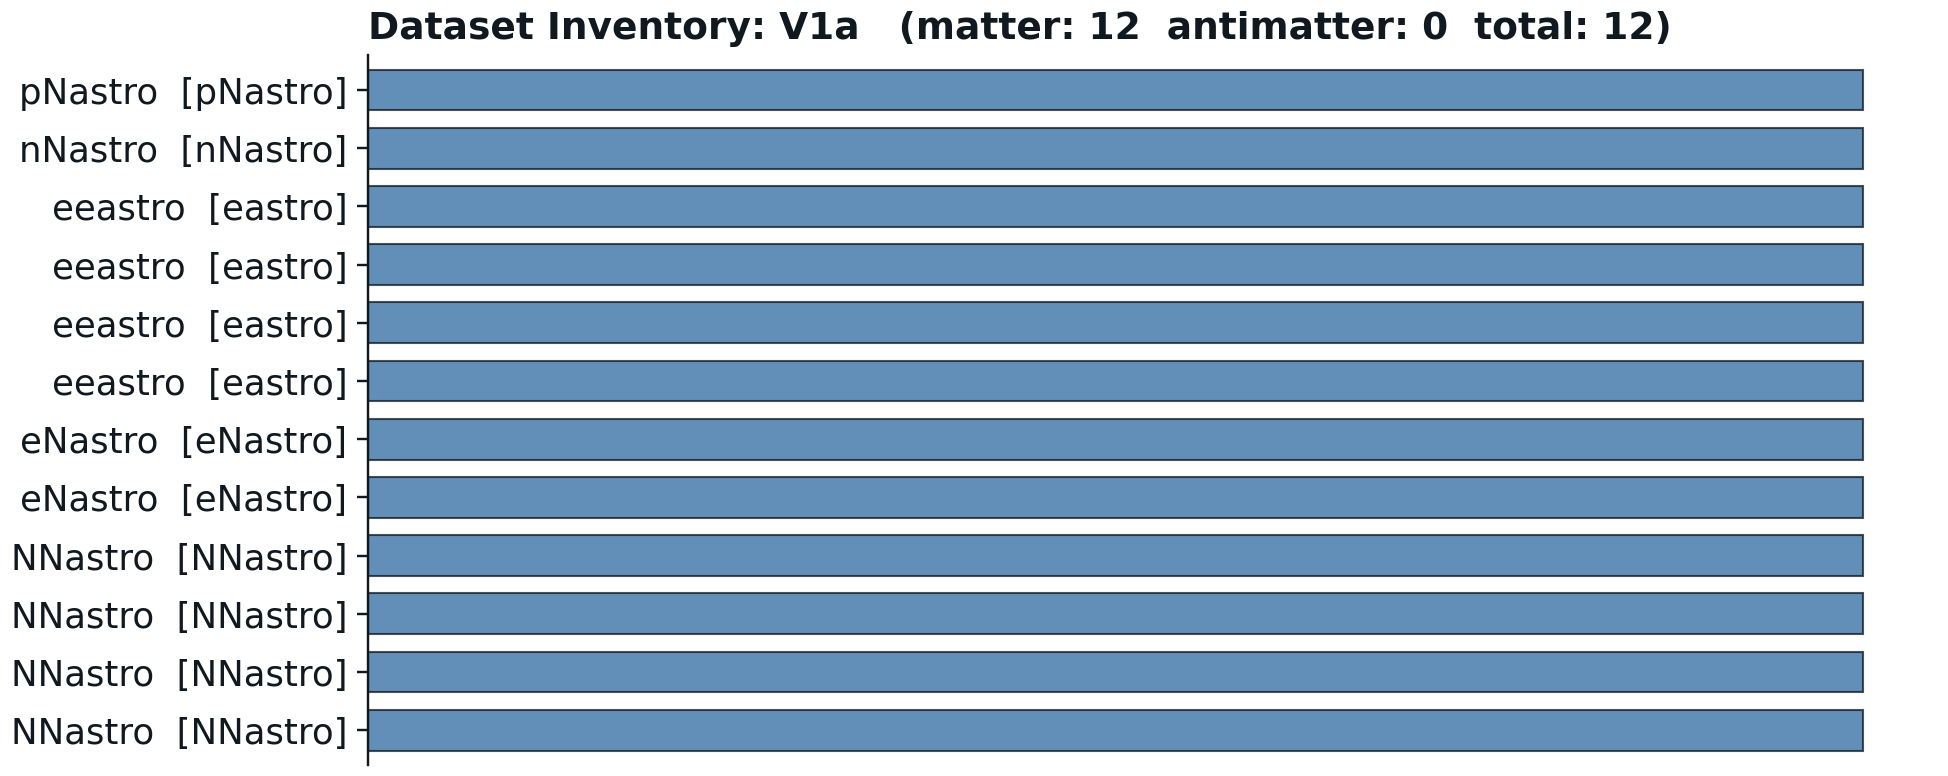
\includegraphics[width=0.85\textwidth,height=0.9\textheight,keepaspectratio]{lambda_coverage_V1a.png}
\caption{Dataset inventory for $V_{1a}$.}
\label{fig:lambda-coverage-v1a}
\end{figure}
\clearpage

\begin{figure}[p]
\centering
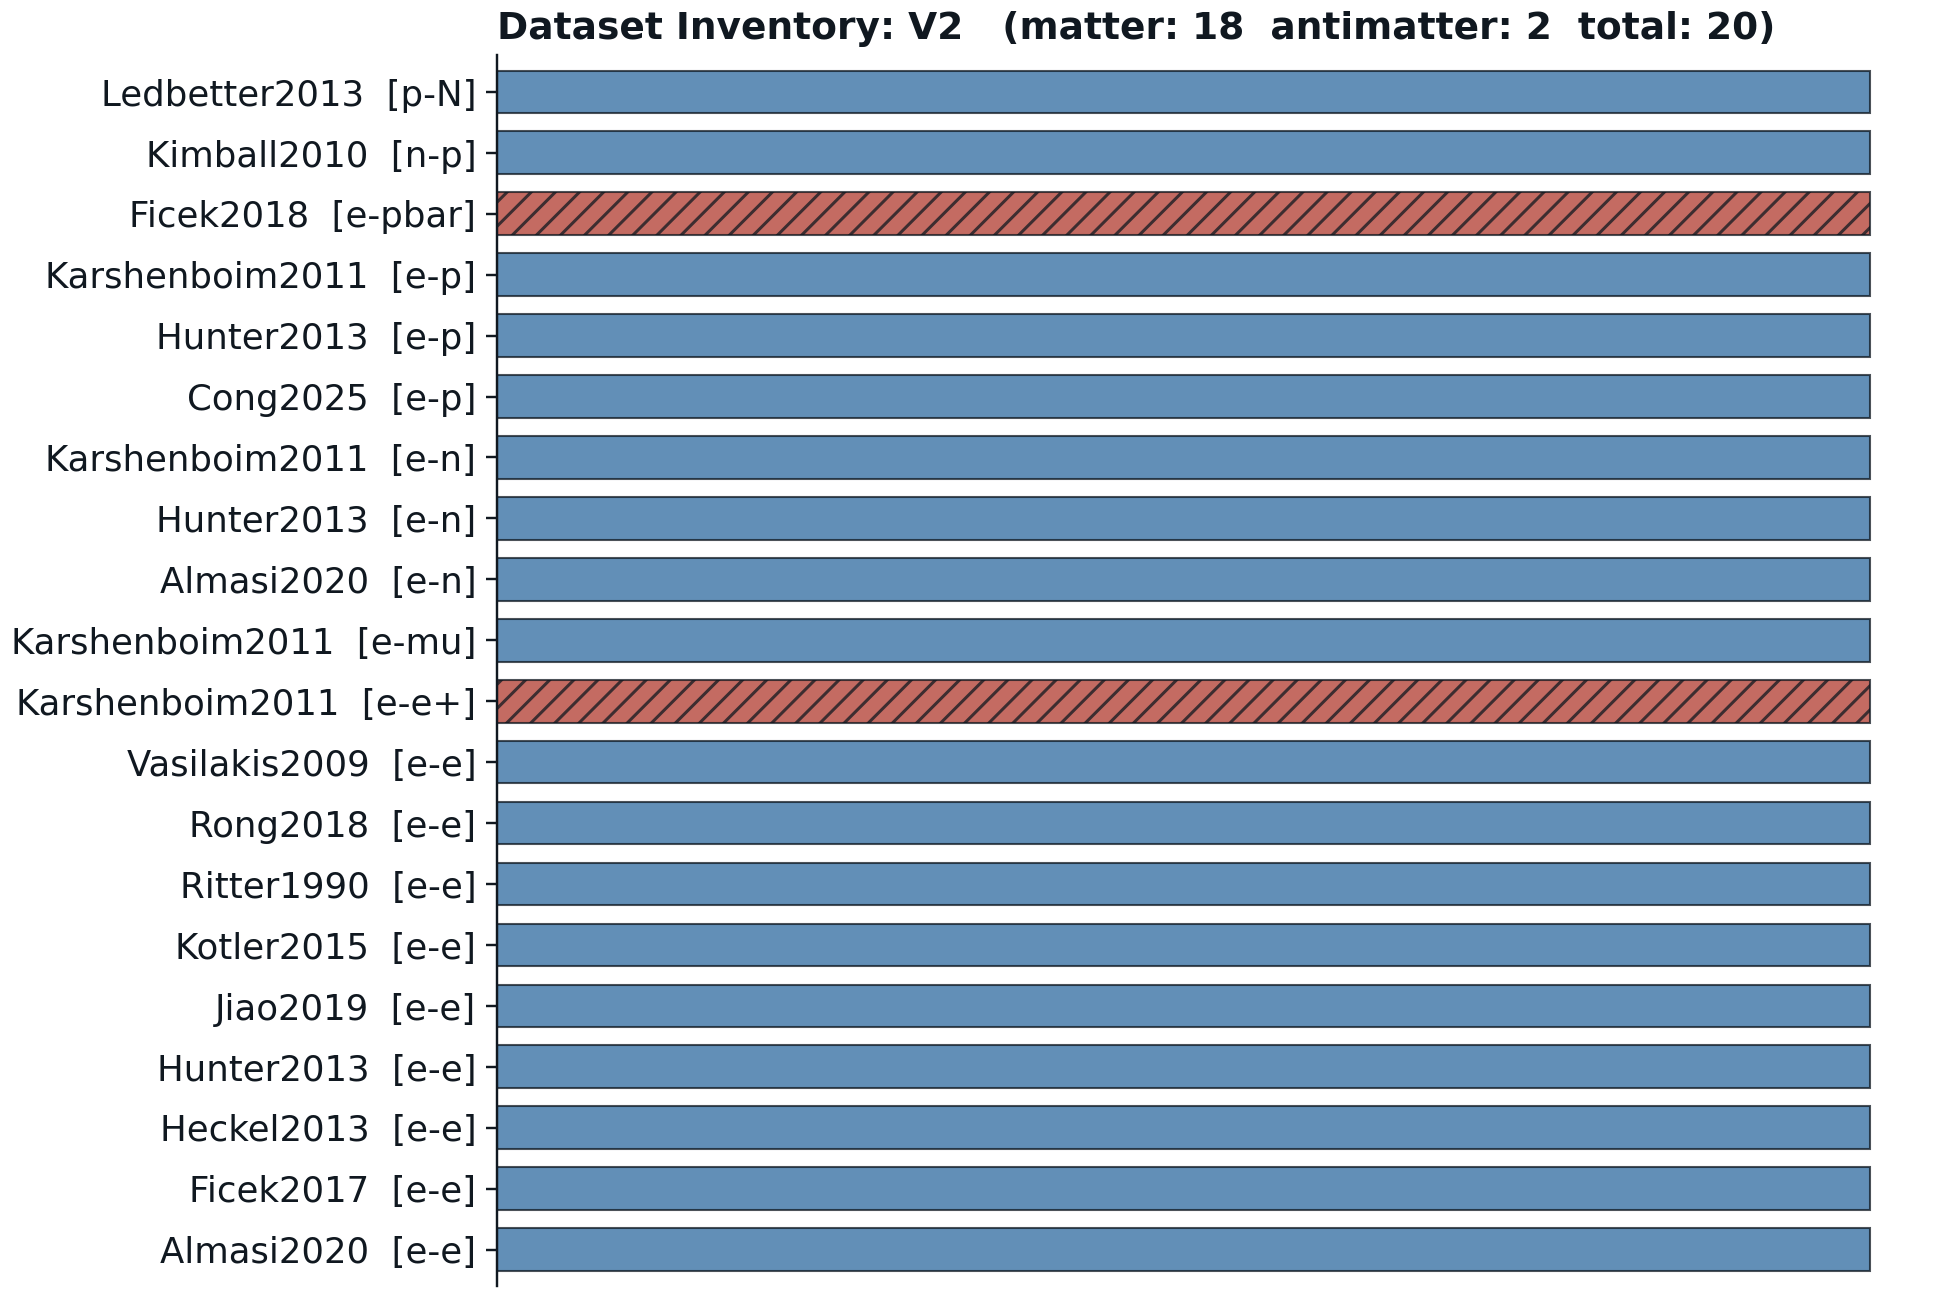
\includegraphics[width=0.85\textwidth,height=0.9\textheight,keepaspectratio]{lambda_coverage_V2.png}
\caption{Dataset inventory for $V_2$.}
\label{fig:lambda-coverage-v2}
\end{figure}
\clearpage

\begin{figure}[p]
\centering
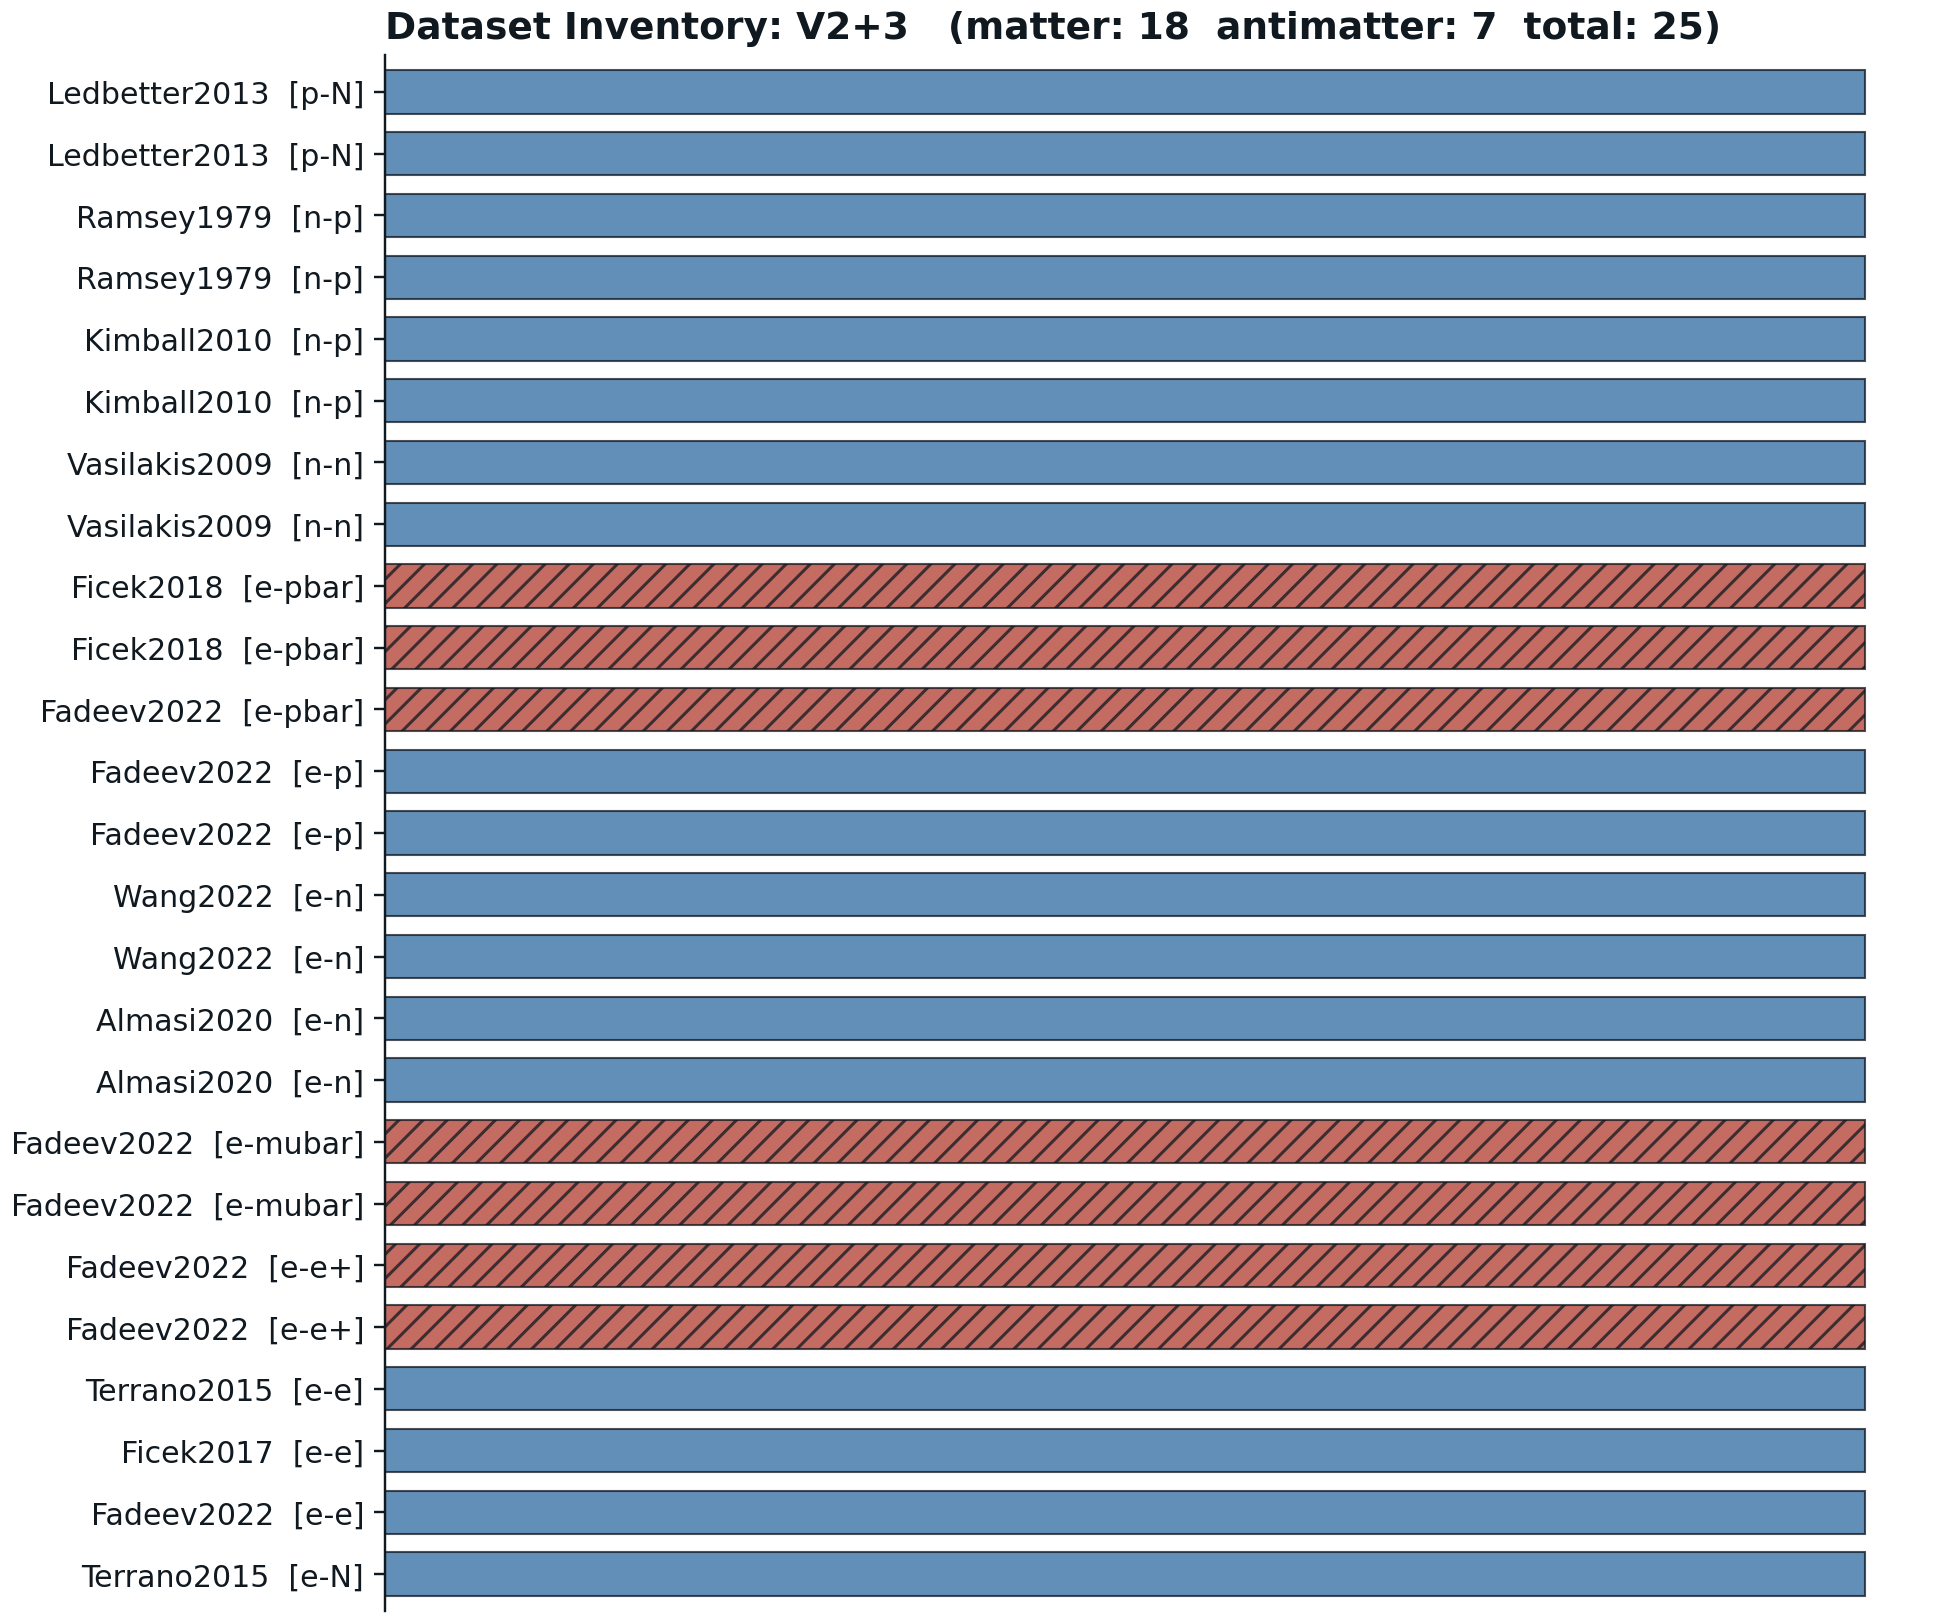
\includegraphics[width=0.85\textwidth,height=0.9\textheight,keepaspectratio]{lambda_coverage_V2p3.png}
\caption{Dataset inventory for $V_{2+3}$.}
\label{fig:lambda-coverage-v2p3}
\end{figure}
\clearpage

\begin{figure}[p]
\centering
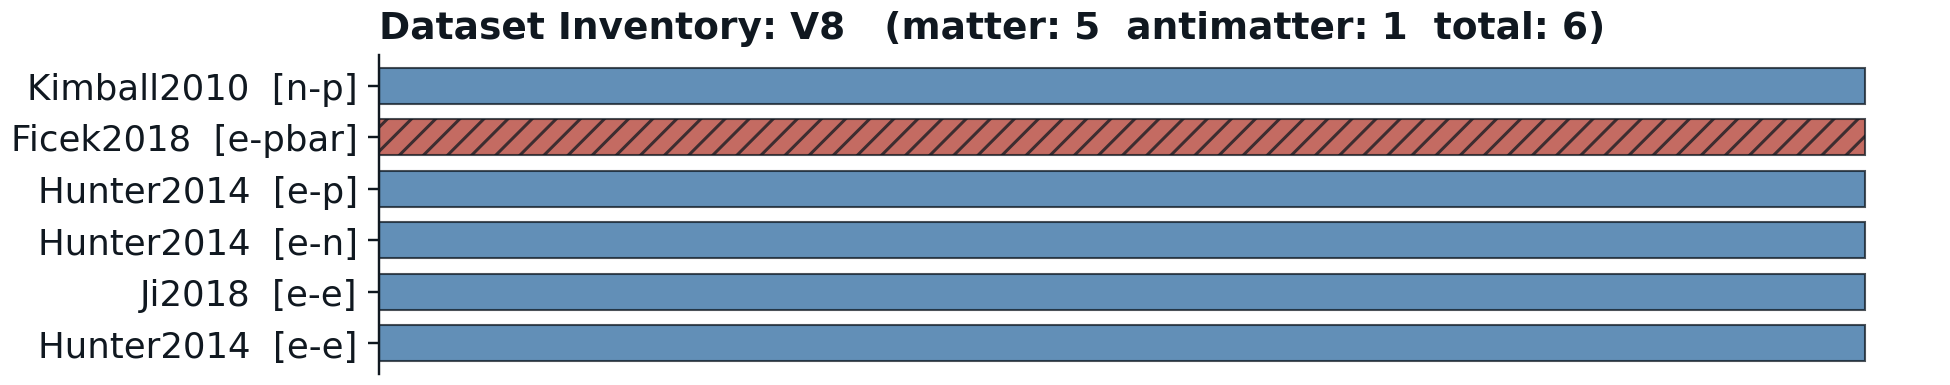
\includegraphics[width=0.85\textwidth,height=0.9\textheight,keepaspectratio]{lambda_coverage_V8.png}
\caption{Dataset inventory for $V_8$.}
\label{fig:lambda-coverage-v8}
\end{figure}
\clearpage

\begin{figure}[p]
\centering
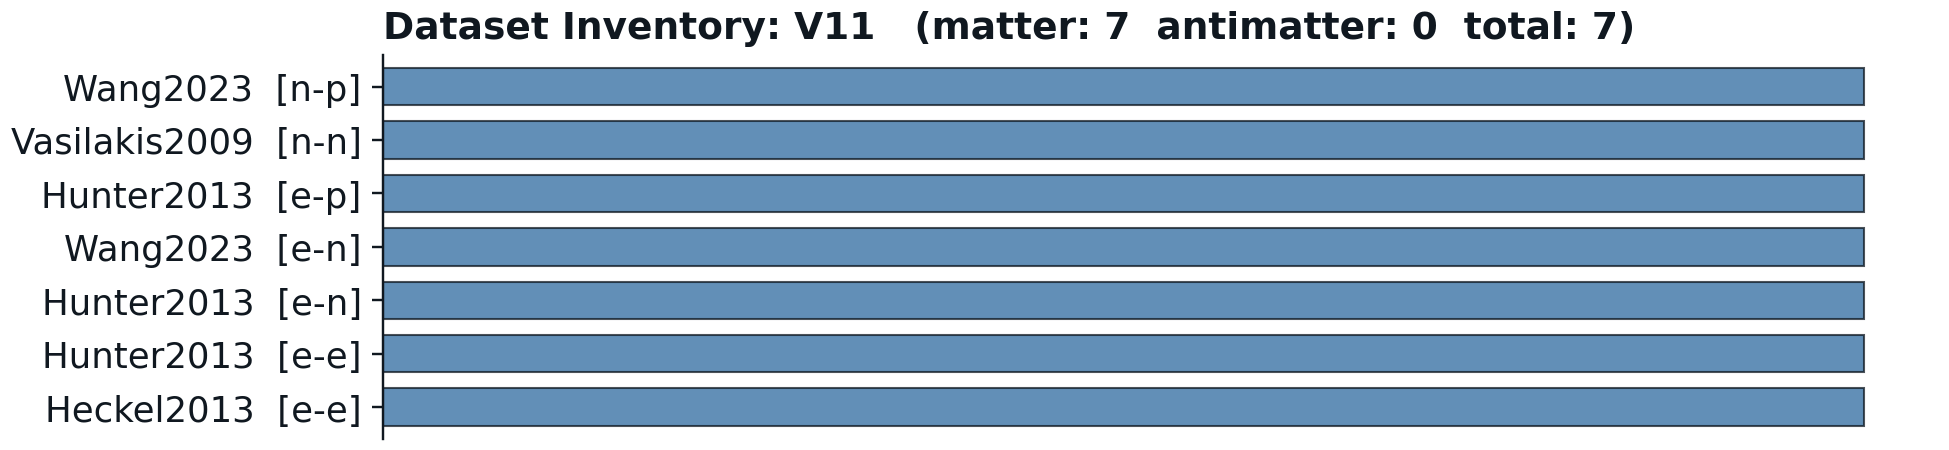
\includegraphics[width=0.85\textwidth,height=0.9\textheight,keepaspectratio]{lambda_coverage_V11.png}
\caption{Dataset inventory for $V_{11}$.}
\label{fig:lambda-coverage-v11}
\end{figure}
\clearpage

\begin{figure}[p]
\centering
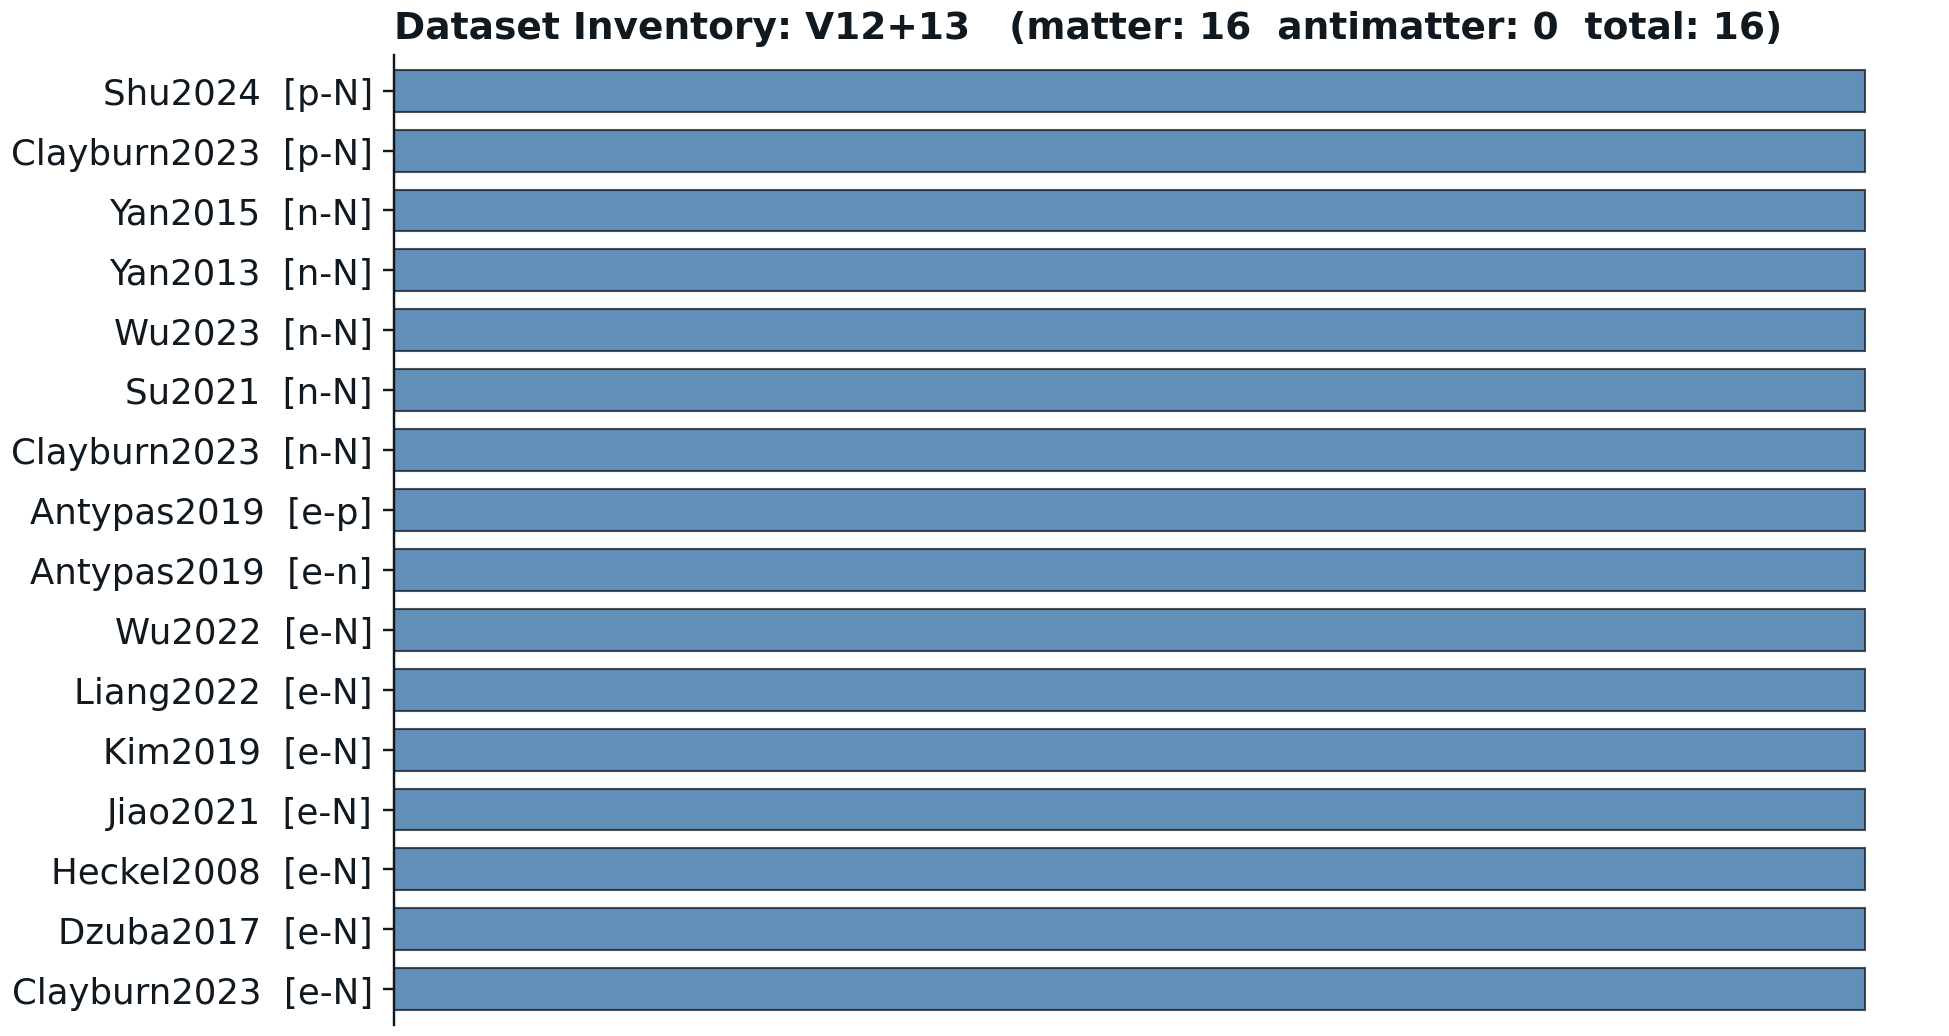
\includegraphics[width=0.85\textwidth,height=0.9\textheight,keepaspectratio]{lambda_coverage_V12p13.png}
\caption{Dataset inventory for $V_{12+13}$.}
\label{fig:lambda-coverage-v12p13}
\end{figure}
\clearpage

\begin{figure}[p]
\centering
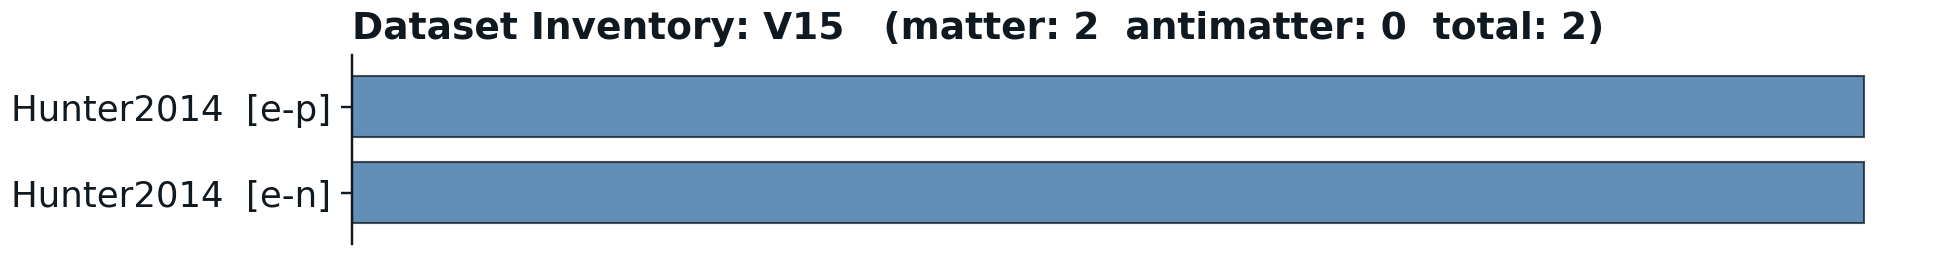
\includegraphics[width=0.7\textwidth]{lambda_coverage_V15.png}
\caption{Dataset inventory for $V_{15}$.}
\label{fig:lambda-coverage-v15}
\end{figure}
\clearpage

\begin{figure}[p]
\centering
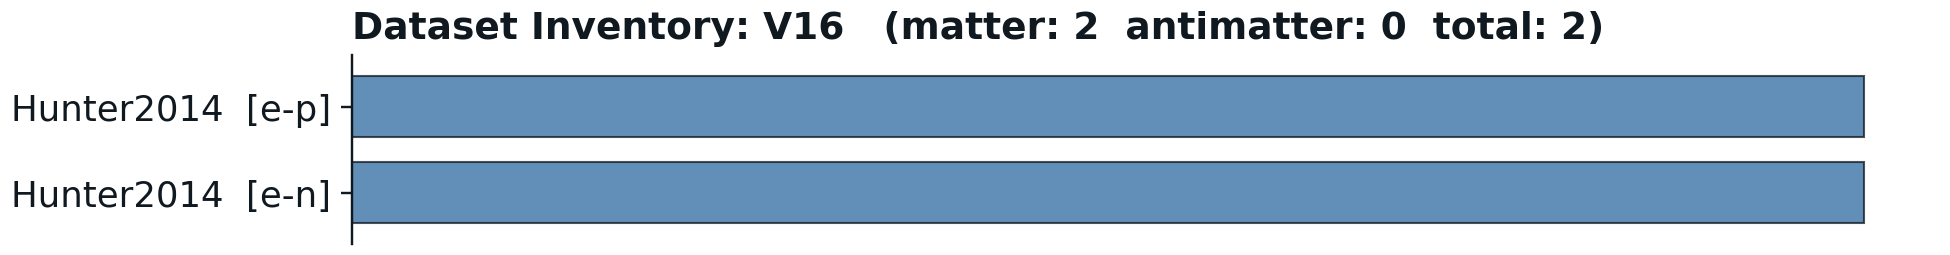
\includegraphics[width=0.7\textwidth]{lambda_coverage_V16.png}
\caption{Dataset inventory for $V_{16}$.}
\label{fig:lambda-coverage-v16}
\end{figure}
\clearpage


\end{document}
